 % Anonymized submission
\documentclass[final,12pt]{colt2018}


% The following packages will be automatically loaded:
% amsmath, amssymb, natbib, graphicx, url, algorithm2e

\title[Outlier-Robust Regression]{Efficient Algorithms for Outlier-Robust Regression}
\usepackage{times}
\usepackage{algorithm}
 % Use \Name{Author Name} to specify the name.
 % If the surname contains spaces, enclose the surname
 % in braces, e.g. \Name{John {Smith Jones}} similarly
 % if the name has a "von" part, e.g \Name{Jane {de Winter}}.
 % If the first letter in the forenames is a diacritic
 % enclose the diacritic in braces, e.g. \Name{{\'E}louise Smith}

 % Two authors with the same address
  % \coltauthor{\Name{Author Name1} \Email{abc@sample.com}\and
  %  \Name{Author Name2} \Email{xyz@sample.com}\\
  %  \addr Address}

 % Three or more authors with the same address:
 % \coltauthor{\Name{Author Name1} \Email{an1@sample.com}\\
 %  \Name{Author Name2} \Email{an2@sample.com}\\
 %  \Name{Author Name3} \Email{an3@sample.com}\\
 %  \addr Address}


 % Authors with different addresses:
 \coltauthor{\Name{Adam Klivans} \Email{klivans@cs.utexas.edu}\\
 \addr University of Texas at Austin
 \AND
 \Name{Pravesh K. Kothari} \Email{kothari@cs.princeton.edu}\\
 \addr Princeton University and IAS
 \AND
 \Name{Raghu Meka} \Email{raghum@cs.ucla.edu}\\
 \addr University of California, Los Angeles
 }







% Acknowledgments---Will not appear in anonymized version

% change to 11pt for conference submission

\usepackage{turnstile}
\usepackage{mdframed}
\usepackage{microtype}

% options for preamble
\def\showauthornotes{0}
\def\showtableofcontents{0}
\def\showkeys{0}
\def\showdraftbox{0}
\def\showcolorlinks{0}
\def\usemicrotype{1}
\def\showfixme{0}
\def\showdefine{0}
%\def\writemode{0}

% Custom commands
\newcommand{\bR}{\mathbb{R}}
\newcommand{\mL}{\mathcal{L}}
\newcommand{\mO}{\mathcal{O}}
\newcommand{\mG}{\mathcal{G}}
\newcommand{\mF}{\mathcal{F}}
\newcommand{\mP}{\mathcal{P}}
\newcommand{\mR}{\mathcal{R}}
\newcommand{\bI}{\mathbf{1}}
\newcommand{\TV}{d_{\text{TV}}}
\newcommand{\KL}{d_{\text{KL}}}
\newcommand{\Tr}{\text{Tr}}
\newcommand{\bP}{\mathbb{P}}
\newcommand{\bE}{\mathbb{E}}

\newcommand{\N}{\mathcal{N}}
\newcommand{\Id}{\mathsf{I}}
\newcommand{\las}{\mathsf{las}}
\newcommand{\spca}{\mathsf{spca}}

\newcommand{\Yt}{\widetilde{Y}}
\newcommand{\Wt}{\widetilde{W}}


% Standard environments
%\newtheorem{definition}{Definition}[section]
%\newtheorem{example}{Example}[section]
%\newtheorem{exercise}{Exercise}[section]
\newtheorem{fact}{Fact}[section]
%\newtheorem{theorem}{Theorem}[section]
%\newtheorem{corollary}{Corollary}[section]
%\newtheorem{conjecture}{Conjecture}[section]
%\newtheorem{lemma}{Lemma}[section]
%\newtheorem{problem}{Problem}[section]
\newenvironment{solution}[1][Solution]{
    \begin{proof}[#1]
  }{
    \end{proof}
  }

\newenvironment{fminipage}%
  {\begin{Sbox}\begin{minipage}}%
  {\end{minipage}\end{Sbox}\fbox{\TheSbox}}

\newenvironment{algbox}[0]{\vskip 0.2in
\noindent 
 \begin{fminipage}{5.9in}
}{
\end{fminipage}
\vskip 0.2in
}

\setcounter{tocdepth}{1}
% algorithm packages



 \usepackage{algorithm}
 %\usepackage{algorithmic}
% %\usepackage{algpseudocode}

% \algnewcommand\algorithmicinput{\textbf{Input:}}
% \algnewcommand\INPUT{\item[\algorithmicinput]}
% \algnewcommand\algorithmicoutput{\textbf{Output:}}
% \algnewcommand\OUTPUT{\item[\algorithmicoutput]}

% paper-specific packages
\usepackage{relsize}
\usepackage[font=footnotesize]{caption}
\usepackage{appendix}


% abbreviations and paper-specific macros

% math
\newcommand{\D}{\mathcal{D}}
\newcommand{\sphere}{\bbS^{n-1}}
\DeclareMathOperator{\Span}{Span}
\DeclareMathOperator{\im}{im}
\DeclareMathOperator{\lamax}{\lambda_{\mathrm{max}}}
\newcommand{\Sn}{\mathbb{S}^{n-1}}
\DeclareMathOperator{\Id}{\mathrm{Id}}
\DeclareMathOperator{\F}{\mathbb{F}}
\DeclareMathOperator{\codim}{codim}

% not math
\DeclareUrlCommand\email{}
\newcommand{\whp}{\text{w.h.p.}}
\newcommand{\wovp}{\text{w.ov.p.}\xspace}
\newcommand{\YES}{\textsc{yes}\xspace}
\newcommand{\NO}{\textsc{no}\xspace}

\newcommand{\wovple}{\hspace{-3mm}\stackrel{\text{\wovp}}{\le}}
\newcommand{\wovpeq}{\hspace{-3mm}\stackrel{\text{\wovp}}{=}}
\newcommand{\wovpge}{\hspace{-3mm}\stackrel{\text{\wovp}}{\ge}}
\newcommand{\aasle}{\hspace{-1.5mm}\stackrel{\text{a.a.s.}}\le}

\newcommand{\Pisymm}{\Pi_{\mathrm{symm}}}
\newcommand{\Pisym}{\Pi_{\mathrm{sym}}}

%added by TM
\newcommand{\inner}[1]{\langle #1 \rangle}
\newcommand{\sosle}{\preceq}
\newcommand{\sosge}{\succeq}

\DeclareMathOperator{\tE}{\tilde{\mathbb E}}
\DeclareMathOperator{\tO}{\tilde{O}}
\DeclareMathOperator{\zo}{\{0,1\}}


\DeclareMathOperator*{\pE}{\widetilde{\mathbb E}}
\DeclareMathOperator*{\pPr}{\widetilde{\mathbb P}}
\DeclareMathOperator*{\pVar}{\widetilde{{\mathbb V}{\mathbb A}{\mathbb R}}}

\newcommand{\bT}{\mathbf{T}}
\newcommand{\ot}{\otimes}
\newcommand{\tr}{\textup{tr}}
\newcommand{\diag}{\textup{diag}}

\let\pref=\prettyref

% transpose
% http://tex.stackexchange.com/questions/204892/visually-appealing-subscripts-with-intercal
% http://tex.stackexchange.com/questions/30619/what-is-the-best-symbol-for-vector-matrix-transpose
\newcommand*{\transpose}[1]{{#1}{}^{\mkern-4mu\intercal}}
\newcommand*{\vardyad}[1]{#1^{\vphantom{\intercal}}#1^{\intercal}}
\newcommand*{\dyad}[1]{#1#1{}^{\mkern-4mu\intercal}}

% \let\Id\undefined
% \newcommand*{\Id}{I}

% span of subspace -- temporary

\newcommand{\sspan}{\textup{span}}
\newcommand{\1}{\bm{1}}
\newcommand{\bset}{\cB}

%%% Local Variables:
%%% mode: latex
%%% TeX-master: "../planted"
%%% End:

% left-right wrappers
\DeclarePairedDelimiter\parens{\lparen}{\rparen}
\DeclarePairedDelimiter\absryan{\lvert}{\rvert}
\DeclarePairedDelimiter\normryan{\lVert}{\rVert}
\DeclarePairedDelimiter\floor{\lfloor}{\rfloor}
\DeclarePairedDelimiter\ceil{\lceil}{\rceil}
\DeclarePairedDelimiter\braces{\lbrace}{\rbrace}
\DeclarePairedDelimiter\bracks{\lbrack}{\rbrack}
\DeclarePairedDelimiter\angles{\langle}{\rangle}

\newcommand{\wt}[1]{\widetilde{#1}}
\newcommand{\wh}[1]{\widehat{#1}}
\newcommand{\avg}{\mathop{\mathrm{avg}}}

\newcommand{\littlesum}{\mathop{{\textstyle \sum}}}
\newcommand{\littleprod}{\mathop{{\textstyle \prod}}}

% calligraphic letters
\newcommand{\calA}{\mathcal{A}}
\newcommand{\calB}{\mathcal{B}}
\newcommand{\calC}{\mathcal{C}}
\newcommand{\calD}{\mathcal{D}}
\newcommand{\calE}{\mathcal{E}}
\newcommand{\calF}{\mathcal{F}}
\newcommand{\calG}{\mathcal{G}}
\newcommand{\calH}{\mathcal{H}}
\newcommand{\calI}{\mathcal{I}}
\newcommand{\calJ}{\mathcal{J}}
\newcommand{\calK}{\mathcal{K}}
\newcommand{\calL}{\mathcal{L}}
\newcommand{\calM}{\mathcal{M}}
\newcommand{\calN}{\mathcal{N}}
\newcommand{\calO}{\mathcal{O}}
\newcommand{\calP}{\mathcal{P}}
\newcommand{\calQ}{\mathcal{Q}}
\newcommand{\calR}{\mathcal{R}}
\newcommand{\calS}{\mathcal{S}}
\newcommand{\calT}{\mathcal{T}}
\newcommand{\calU}{\mathcal{U}}
\newcommand{\calV}{\mathcal{V}}
\newcommand{\calW}{\mathcal{W}}
\newcommand{\calX}{\mathcal{X}}
\newcommand{\calY}{\mathcal{Y}}
\newcommand{\calZ}{\mathcal{Z}}

% bold
\newcommand{\bone}{\boldsymbol{1}}
\newcommand{\bbeta}{\boldsymbol{\beta}}
\newcommand{\bdelta}{\boldsymbol{\delta}}
\newcommand{\bepsilon}{\boldsymbol{\epsilon}} \newcommand{\beps}{{\bepsilon}}
\newcommand{\blambda}{\boldsymbol{\lambda}}
\newcommand{\bomega}{\boldsymbol{\omega}}
\newcommand{\bpi}{\boldsymbol{\pi}}
\newcommand{\bphi}{\boldsymbol{\phi}}
\newcommand{\bvphi}{\boldsymbol{\varphi}}
\newcommand{\bpsi}{\boldsymbol{\psi}}
\newcommand{\bsigma}{\boldsymbol{\sigma}}
\newcommand{\btheta}{\boldsymbol{\theta}}
\newcommand{\ba}{\boldsymbol{a}}
\newcommand{\bb}{\boldsymbol{b}}
\newcommand{\bc}{\boldsymbol{c}}
\newcommand{\bd}{\boldsymbol{d}}
\newcommand{\be}{\boldsymbol{e}}
\newcommand{\boldf}{\boldsymbol{f}}
\newcommand{\bg}{\boldsymbol{g}}
\newcommand{\bh}{\boldsymbol{h}}
\newcommand{\bi}{{\boldsymbol{i}}}
\newcommand{\bj}{{\boldsymbol{j}}}
\newcommand{\bk}{{\boldsymbol{k}}}
\newcommand{\bell}{{\boldsymbol{\ell}}}
\newcommand{\bp}{\boldsymbol{p}}
\newcommand{\br}{\boldsymbol{r}}
\newcommand{\bs}{\boldsymbol{s}}
\newcommand{\bt}{\boldsymbol{t}}
\newcommand{\bu}{\boldsymbol{u}}
\newcommand{\bv}{\boldsymbol{v}}
\newcommand{\bw}{\boldsymbol{w}}
\newcommand{\bx}{{\boldsymbol{x}}}
\newcommand{\boldy}{\boldsymbol{y}}
\newcommand{\bz}{\boldsymbol{z}}
\newcommand{\bA}{\boldsymbol{A}}
\newcommand{\bB}{\boldsymbol{B}}
\newcommand{\bC}{\boldsymbol{C}}
\newcommand{\bD}{\boldsymbol{D}}
\newcommand{\bE}{\boldsymbol{E}}
\newcommand{\bF}{\boldsymbol{F}}
\newcommand{\bG}{\boldsymbol{G}}
\newcommand{\bH}{\boldsymbol{H}}
\newcommand{\bI}{\boldsymbol{I}}
\newcommand{\bJ}{\boldsymbol{J}}
\newcommand{\bL}{\boldsymbol{L}}
\newcommand{\bM}{\boldsymbol{M}}
\newcommand{\bP}{\boldsymbol{P}}
\newcommand{\bR}{\boldsymbol{R}}
\newcommand{\bS}{\boldsymbol{S}}
\newcommand{\boldT}{\boldsymbol{T}}
\newcommand{\bU}{\boldsymbol{U}}
\newcommand{\bV}{\boldsymbol{V}}
\newcommand{\bX}{\boldsymbol{X}}
\newcommand{\bY}{\boldsymbol{Y}}
\newcommand{\bZ}{\boldsymbol{Z}}

%%%%%%%%%%%

\newcommand{\OBJ}{\mathrm{OBJ}} 

\newcommand{\ignore}[1]{}

\renewcommand{\H}{\mathcal{H}}
\newcommand{\dtensor}{\circledast}
\renewcommand{\S}{\mathbb{S}}
\newcommand{\rnote}[1]{\footnote{\color{blue}Ryan: {#1}}}
\newcommand{\mnote}{\Authornote{M}}
%\newcommand{\rnote}[1]{}
\newcommand{\CONSMALL}{\scalebox{.75}[1.0]{\textnormal{SMALL}}}
\newcommand{\cons}{\mathrm{cons}}
\newcommand{\cl}{\mathrm{cl}}
\newcommand{\tmu}{\tilde{\mu}}
\renewcommand{\pE}{\tilde{\mathbb{E}}}
\newcommand{\err}{\mathsf{err}}

\makeatletter
\def\blfootnote{\xdef\@thefnmark{}\@footnotetext}
\makeatother


\setcounter{page}{1}

% \title{Regression Algorithms Robust to Adversarial, Outlier Corruptions\footnote{}}

% \author{Adam R. Klivans \thanks{UT Austin \texttt{klivans@cs.utexas.edu}}
% \and Pravesh K. Kothari\thanks{Princeton University and Institute for Advanced Study. \texttt{kothari@cs.princeton.edu}.} \and Raghu Meka \thanks{University of California, Los Angeles \texttt{raghum@cs.ucla.edu}}}

%\date{}

\setcounter{tocdepth}{2}

\begin{document}

\maketitle \blfootnote{Extended abstract. Full version appears as [arXiv 1803.03241 v3]}





We present preconditioned stochastic gradient descent (SGD) algorithms for the $\ell_1$ minimization problem $\min_{\xx}\|\AA \xx - \bb\|_1$ in the overdetermined case, where there are far more constraints than variables. Specifically, we have $\AA \in \R^{n \times d}$ for $n \gg d$. Commonly known as the Least Absolute Deviations problem, $\ell_1$ regression can be used to solve many important combinatorial problems, such as minimum cut and shortest path. SGD-based algorithms are appealing for their simplicity and practical efficiency.
% Our algorithms precondition the matrix $\AA$ and then solve the problem for the resulting matrix $\tilde{\AA}$ using gradient descent techniques.
Our primary insight is that careful preprocessing can yield preconditioned matrices $\tilde{\AA}$ with strong properties (besides good condition number and low-dimension) that allow for faster convergence of gradient descent. In particular, we precondition using Lewis weights to obtain an isotropic matrix with fewer rows and strong upper bounds on all row norms. We leverage these conditions to find a good initialization, which we use along with recent smoothing reductions and accelerated stochastic gradient descent algorithms to achieve $\epsilon$ relative error in $\Otil(nnz(\AA) + d^{2.5} \epsilon^{-2})$ time with high probability, where $nnz(\AA)$ is the number of non-zeros in $\AA$. This improves over the previous best result using gradient descent for $\ell_1$ regression. We also match the best known running times for interior point methods in several settings.

Finally, we also show that if our original matrix $\AA$ is approximately isotropic and the row norms are approximately equal, we can give an algorithm that avoids using fast matrix multiplication and obtains a running time of $\Otil(nnz(\AA) + s d^{1.5}\epsilon^{-2} + d^2\epsilon^{-2})$, where $s$ is the maximum number of non-zeros in a row of $\AA$. In this setting, we beat the best interior point methods for certain parameter regimes.


%We consider the $\ell_1$ minimization problem $\min_{\xx}||\AA \xx - \bb||_1$ in the overconstrained case, where there are far more constraints than variables. More specifically, we have $\AA \in \R^{n \times d}$ for $n \gg d$. By using Lewis Weights preconditioning on $\AA$ and a careful initialization, we show that a standard stochastic gradient descent algorithm achieves $\epsilon$ relative error in about $nnz(\AA) +  d^3\epsilon^{-2}$ time with high probability. If we leverage smoothing reductions in \cite{AllenZhuH16} and the accelerated stochastic gradient descent algorithms in \cite{AllenZhu17}, we can achieve a running time of about $nnz(\AA) + d^{2.5}\epsilon^{-2}$ with the same guarantees. Both of these running times improve over the previous results in \cite{YangCRM16} and the latter result is comparable to the best known running times for interior point methods \cite{LeeS15}.
%
%The key idea will be to use our preconditioning to restrict our consideration to matrices $\AA$ such that $\AA^T\AA = \II$ and every row norm of $\AA$ is upper bounded by $O(\sqrt{d/n})$. \cite{cohenpeng} show that sampling $\AA$ with Lewis weights takes about $nnz(\AA) +d^{\omega}$ time and approximately preserves the minimization problem. Moreover, we can assume $n\le O(d\epsilon^{-2}\log n)$ for the sampled matrix. We then prove that all leverage scores of the sampled matrix are approximately equal. Since rotations preserve leverage scores, we can then rotate our sampled matrix to ensure that our desired properties are met in about $d^{\omega}\epsilon^{-2}$ time.
%
%Finally, we also show that if our original matrix $\AA$ is such that $\AA^T\AA \approx \II$ and the row norms of $\AA$ are bounded, we can avoid using fast matrix multiplication and prove a running time of about $nnz(\AA) + s d^{1.5}\epsilon^{-2}$, where $s$ is the maximum number of non-zeros in a row of $\AA$.

%Consequently, we will be able to restrict our consideration to matrices $A$ such that $A^TA \approx I$, and all row norms are equal, which is to say $||A_{i,:}||_2 = \sqrt{\frac{d}{n}}$ for all $i$.
%
%With a careful choice of our initial $x$, we show that standard gradient descent and stochastic gradient descent algorithms under these further assumptions only require $O(\frac{d}{\epsilon^2})$ and $O(\frac{d^2}{\epsilon^2})$ iterations, respectively, to achieve $\epsilon$ relative error with respect to the minimum objective value. Accordingly, these methods each achieve respective total runtime of $O(\frac{md}{\epsilon^2})$ and $O(\frac{d^3}{\epsilon^2})$, along with an $O(m)$ preconditioning cost, improving over the previous results in \cite{MahoneySGD}.
%
%We further examine the consequences of our assumptions when combined with smoothing reductions in [cite] and accelerated gradient descent techniques in [cite,cite]. As a result we are able to further improve the running times to $O(\frac{md}{\epsilon})$ and $O(dn\log{1/\epsilon} + \frac{d^2\sqrt{n}}{\epsilon})$.
%
%Random sampling $d\epsilon^{-2}\log{d}$ rows of $A$ will only incur error $\epsilon$ and reduces the latter running time to $O(\frac{d^{2.5}\log{d}}{\epsilon^2})$, which is then comparable to interior point methods of [cite]


\begin{keywords}
sum-of-squares, regression, robust learning
\end{keywords}


 \draftbox
\thispagestyle{empty}

%We present preconditioned stochastic gradient descent (SGD) algorithms for the $\ell_1$ minimization problem $\min_{\xx}\|\AA \xx - \bb\|_1$ in the overdetermined case, where there are far more constraints than variables. Specifically, we have $\AA \in \R^{n \times d}$ for $n \gg d$. Commonly known as the Least Absolute Deviations problem, $\ell_1$ regression can be used to solve many important combinatorial problems, such as minimum cut and shortest path. SGD-based algorithms are appealing for their simplicity and practical efficiency.
% Our algorithms precondition the matrix $\AA$ and then solve the problem for the resulting matrix $\tilde{\AA}$ using gradient descent techniques.
Our primary insight is that careful preprocessing can yield preconditioned matrices $\tilde{\AA}$ with strong properties (besides good condition number and low-dimension) that allow for faster convergence of gradient descent. In particular, we precondition using Lewis weights to obtain an isotropic matrix with fewer rows and strong upper bounds on all row norms. We leverage these conditions to find a good initialization, which we use along with recent smoothing reductions and accelerated stochastic gradient descent algorithms to achieve $\epsilon$ relative error in $\Otil(nnz(\AA) + d^{2.5} \epsilon^{-2})$ time with high probability, where $nnz(\AA)$ is the number of non-zeros in $\AA$. This improves over the previous best result using gradient descent for $\ell_1$ regression. We also match the best known running times for interior point methods in several settings.

Finally, we also show that if our original matrix $\AA$ is approximately isotropic and the row norms are approximately equal, we can give an algorithm that avoids using fast matrix multiplication and obtains a running time of $\Otil(nnz(\AA) + s d^{1.5}\epsilon^{-2} + d^2\epsilon^{-2})$, where $s$ is the maximum number of non-zeros in a row of $\AA$. In this setting, we beat the best interior point methods for certain parameter regimes.


%We consider the $\ell_1$ minimization problem $\min_{\xx}||\AA \xx - \bb||_1$ in the overconstrained case, where there are far more constraints than variables. More specifically, we have $\AA \in \R^{n \times d}$ for $n \gg d$. By using Lewis Weights preconditioning on $\AA$ and a careful initialization, we show that a standard stochastic gradient descent algorithm achieves $\epsilon$ relative error in about $nnz(\AA) +  d^3\epsilon^{-2}$ time with high probability. If we leverage smoothing reductions in \cite{AllenZhuH16} and the accelerated stochastic gradient descent algorithms in \cite{AllenZhu17}, we can achieve a running time of about $nnz(\AA) + d^{2.5}\epsilon^{-2}$ with the same guarantees. Both of these running times improve over the previous results in \cite{YangCRM16} and the latter result is comparable to the best known running times for interior point methods \cite{LeeS15}.
%
%The key idea will be to use our preconditioning to restrict our consideration to matrices $\AA$ such that $\AA^T\AA = \II$ and every row norm of $\AA$ is upper bounded by $O(\sqrt{d/n})$. \cite{cohenpeng} show that sampling $\AA$ with Lewis weights takes about $nnz(\AA) +d^{\omega}$ time and approximately preserves the minimization problem. Moreover, we can assume $n\le O(d\epsilon^{-2}\log n)$ for the sampled matrix. We then prove that all leverage scores of the sampled matrix are approximately equal. Since rotations preserve leverage scores, we can then rotate our sampled matrix to ensure that our desired properties are met in about $d^{\omega}\epsilon^{-2}$ time.
%
%Finally, we also show that if our original matrix $\AA$ is such that $\AA^T\AA \approx \II$ and the row norms of $\AA$ are bounded, we can avoid using fast matrix multiplication and prove a running time of about $nnz(\AA) + s d^{1.5}\epsilon^{-2}$, where $s$ is the maximum number of non-zeros in a row of $\AA$.

%Consequently, we will be able to restrict our consideration to matrices $A$ such that $A^TA \approx I$, and all row norms are equal, which is to say $||A_{i,:}||_2 = \sqrt{\frac{d}{n}}$ for all $i$.
%
%With a careful choice of our initial $x$, we show that standard gradient descent and stochastic gradient descent algorithms under these further assumptions only require $O(\frac{d}{\epsilon^2})$ and $O(\frac{d^2}{\epsilon^2})$ iterations, respectively, to achieve $\epsilon$ relative error with respect to the minimum objective value. Accordingly, these methods each achieve respective total runtime of $O(\frac{md}{\epsilon^2})$ and $O(\frac{d^3}{\epsilon^2})$, along with an $O(m)$ preconditioning cost, improving over the previous results in \cite{MahoneySGD}.
%
%We further examine the consequences of our assumptions when combined with smoothing reductions in [cite] and accelerated gradient descent techniques in [cite,cite]. As a result we are able to further improve the running times to $O(\frac{md}{\epsilon})$ and $O(dn\log{1/\epsilon} + \frac{d^2\sqrt{n}}{\epsilon})$.
%
%Random sampling $d\epsilon^{-2}\log{d}$ rows of $A$ will only incur error $\epsilon$ and reduces the latter running time to $O(\frac{d^{2.5}\log{d}}{\epsilon^2})$, which is then comparable to interior point methods of [cite]



%\clearpage



% tableofcontents added for better navigability of the document
\ifnum\showtableofcontents=1
{
\tableofcontents
\thispagestyle{empty}
 }
\fi

%\clearpage

\newtheorem{algorithms}[theorem]{Algorithm}

\setcounter{page}{1}
% !TeX root = main.tex
\section{Introduction}
\label{sec:intro}
Generative models are often trained in an unsupervised fashion, fitting a model $q$ to a set of observed data $x_P \subseteq X$ drawn iid from some true distribution $p$ on $x\in X$. Now, of course $p$ may not exactly belong to family $Q$ of probability distributions being fit, whether $Q$ consists of Gaussians mixture models, Markov models, or even neural networks of bounded size. We first discuss the limitations of generative modeling without feedback, and then discuss our model and results.

%\subsection{Limitations of Generative Modeling from Positive Examples Alone}
Consider fitting a generative model on a text corpus consisting partly of poetry written by four-year-olds and partly of mathematical publications from the {\em Annals of Mathematics}. Suppose that learning to generate a poem that looks like it was written by a child was easier than learning to generate a novel mathematical article with a correct, nontrivial statement. If the generative model pays a high price for generating unrealistic examples, then it may be better off learning to generate children's poetry than mathematical publications. However, without negative feedback, it may be difficult for a neural network or any other model to know that the mathematical articles it is generating are stylistically similar to the mathematical publications but do not contain valid proofs.\footnote{This is excluding clearly fake articles published without proper review in lower-tier venues \citep{LabbeL13}.} 

As a simpler example, the classic Markovian ``trigram model'' of natural language assigns each word a fixed probability conditioned only on the previous two words. Prior to recent advances in deep learning, for decades the trigram model and its variant were the workhorses of language modeling, assigning much greater likelihood to natural language corpora than numerous linguistically motivated grammars and other attempts \citep{Rosenfeld00}. However, text sampled from a trigram is typically nonsensical, e.g., the following text was randomly generated from a trigram model fit on a corpus of text from the Wall Street Journal \citep{JurafskyM09}:
\begin{quote}
They also point to ninety nine point six billion dollars from two hundred
four oh six three percent of the rates of interest stores as Mexico and
gram Brazil on market conditions. 
\end{quote}

In some applications, like text compression using a language model \citep{WittenNC87}, maximizing likelihood is equivalent to optimizing compression. However, in many  applications involving generation, such nonsense is costly and unacceptable. Now, of course it is possible to always generate valid data by returning random training examples, but this is simply overfitting and not learning. Alternatively, one could incorporate human-in-the-loop feedback such as through crowdsourcing, into the generative model to determine what is a valid, plausible sentence.

In some domains, validity could be determined automatically. Consider a Markovian model of a well-defined concept such as mathematical formulas that compile in \LaTeX{}. Now, consider a $n$-gram Markovian character model which the probability of each subsequent character is determined by the previous $n$ characters. For instance, the expression \$\{2+\{x-y\}\$ is invalid in \LaTeX{} due to mismatched braces. For this problem, a \LaTeX{} compiler may serve as a validity oracle. Various $n$-gram models can be fit which only generate valid formulas. To address mismatched braces, for example, one such model would ensure that it always closed braces within $n$ characters of opening, and had no nested braces. While an $n$-gram model will not perfectly model the true distribution over valid \LaTeX{} formulas, for certain generative purposes one may prefer an $n$-gram model that generates valid formulas over one that assigns greater likelihood to the training data but generates invalid formulas. 

Figure \ref{fig:rectangle} illustrates a simple case of learning a rectangle model for data which is not uniform over a rectangle. A maximum likelihood model would necessarily be the smallest rectangle containing all the data, but most examples generated from this distribution may be invalid. Instead a smaller rectangle, as illustrated in the figure, may be desired.

\begin{figure}[h]\label{fig:rectangle}
\centering
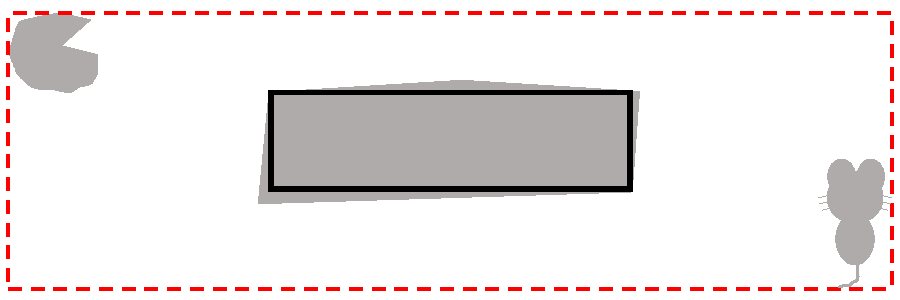
\includegraphics[width=3in]{fig.pdf}
\caption{Example where the underlying distribution $p$ is uniform over the (gray) valid regions. The solid rectangle maximizes our objective since it does not output nonsense (is supported only within the grey matter) and is closest to the $p$ (covers the maximum amount of grey matter). In contrast, the standard maximum likelihood (dashed red) rectangle must fully contain the observed samples, thus generating invalid points most of the time.  }
\end{figure}

Motivated by these observations, we evaluate a generative model $q$ on two axes. First is {\em coverage}, which is related to the probability assigned to future examples drawn from the true distribution $p$. Second is {\em validity}, defined as the probability that random examples generated from $q$ meet some validity requirement. Formally, we measure coverage in terms of a bounded {\em loss}:
$$\Loss(p,q)=\E_{x \sim p}[L(q_x)],$$
where $L:[0,1]\rightarrow [0,M]$ is a bounded decreasing function such as the capped log-loss $L(q_x)=\min(M, \log 1/q_x)$. % or $L(q_x)=\log 1/(q_x+\exp(-M))$. 
A bounded loss has the advantages of being efficiently estimable, and also it enables a model to assign 0 probability to one example (e.g., an outlier or error) if it greatly increases the likelihood of all other data. Validity is defined with respect to a set $V \subseteq X$, and $q(V)$ is the probability that a random example generated from $q$ lies within $V$. 

Clearly, there is a tradeoff between coverage and validity. We first focus on the case of (near) perfect validity. A Valid Generative Modeling (VGM) algorithm if it outputs, for a family of distributions $Q$ over $X$, if it outputs $\hat{q}$ with (nearly) perfect validity and whose loss is nearly as good as the loss of the best valid $q\in Q$. More precisely, $A$ is a VGM learner of $Q$ if for any nonempty valid subset $V \subseteq X$, any probability distribution $p$ over $V$, and any $\eps>0$, $A$ uses $n$ random samples from $p$ and makes $m$ membership oracle calls to $V$ and outputs a distribution $\hat{q}$ such that, $$\Loss(p, \hat{q}) \leq \min_{q \in Q: q(V)=1}\Loss(p,q) + \eps ~\text{ and }~\hat{q}(V)\geq 1-\eps.$$ 
We aim for our learner to be sample and query efficient, requiring that $n$ and $m$ are polynomial in $M, 1/\eps$ and a measure of complexity of our distribution class $Q$.
Furthermore, we would like our algorithms to be computationally efficient, with a runtime polynomial in the size of the data, namely the $n + m$ training examples. 
A more formal description of the problem is available in Section~\ref{sec:problem}.

$A$ is said to be {\em proper} if it always outputs $\hat{q}\in Q$ and {\em improper} otherwise.
In Section~\ref{sec:impossibility}, we first show that efficient proper learning for VGM is impossible. This is an information-theoretic result, meaning that even given infinite runtime and positive samples, one still cannot solve the VGM problem. Interestingly, this is different from binary classification, where it is possible to statistically learn from iid examples without a membership oracle.

Our first main positive result is an efficient (improper) learner for VGM. The algorithm relies on a subroutine that solves the following {\em Generative Modeling with Negatives} (GMN) problem: given sets $X_P, X_N \subset X$ of positive and negative examples, find the probability distribution $q \in Q$ which minimizes $\sum_{x \in X_P} L(q(x))$ subject to the constraint that $q(X_N)=0$. For simplicity, we present our algorithm for the case that the distribution family $Q$ is finite, giving sample and query complexity bounds that are logarithmic in terms of $|Q|$. However, as we show in Section~\ref{sec:infinite-families}, all of our results extend to infinite families $Q$. It follows that if one has a computationally efficient algorithm for the GMN problem for a distribution family $Q$, then our reduction gives a computationally efficient VGM learning algorithm for $Q$.

Our second positive result is an algorithm that minimizes $\Loss(p,q)$ subject to a relaxed validity constraint comparing against the optimal distribution that has validity $q(V)$ at least $1-\alpha$ for some $\alpha>0$. We show in Section~\ref{sec:partial-validity} that even in this more general setting, it is possible to obtain an algorithm that is statistically efficient but may not be computationally efficient. An important open question is whether there exists a computationally efficient algorithm for this problem when given access to an optimization oracle, as was the case for our algorithm for VGM.

\subsection{Related Work}
\cite{KearnsMRRSS94} showed how to learn distributions from positive examples in the realizable setting, i.e., where the true distribution is assumed to belong to the class being learned. In the same sense as their work is similar to PAC learning \citet{Valiant84} of distributions, our work is like agnostic learning \citet{KearnsSS94} in which no assumption on the true distribution is made. 

Generative Adversarial Networks (GANs)~\cite{GoodfellowPMXWOCB14} are an approach for generative modeling from positive examples alone, in which a generative model is trained against a discriminator that aims to distinguish real data from generated data. In some domains, GANs have been shown to outperform other methods at generating realistic-looking examples. Several shortcomings of GANs have been observed \citet{AroraRZ18}, and GANs are still subject to the theoretical limitations we argue are inherent to any model trained without a validity oracle. 

In supervised learning, there is a rich history of learning theory with various types of queries, including membership which are not unlike our (in)validity oracle. Under various assumptions, queries have been shown to facilitate the learning of complex classes such as finite automata \citet{Angluin88} and DNFs \citet{Jackson97}. See the survey of \cite{Angluin92} for further details.  Interestingly, \cite{Feldman09} has shown that for agnostic learning, i.e., without making assumptions on the generating distribution, the addition of membership queries does not enhance what is learnable beyond random examples alone. 
Supervised learning also has a large literature around active learning, showing how the ability to query examples reduces the sample complexity of many algorithms. See the survey of \cite{Hanneke14}. Note that the aim here is typically to save examples and not to expand what is learnable.
 
More sophisticated models, e.g., involving neural networks, can mitigate the invalidity problem as they often generate more realistic natural language and have even been demonstrated to generate \LaTeX{} that nearly compiles \citep{Karpathy15} or nearly valid Wikipedia markdown. However, longer strings generated are unlikely to be valid. For example, \cite{Karpathy15} shows generated markdown which includes:
\begin{quote}
==Access to ''rap===
The current history of the BGA has been [[Vatican Oriolean Diet]], British Armenian, published in 1893.  While actualistic such conditions such as the [[Style Mark Romanians]] are still nearly not the loss.
\end{quote}

Even ignoring the mismatched quotes and equal signs, note that this example has two so-called ``red links'' to two pages that do not exist. Without checking, it was not obvious to us whether or not Wikipedia had pages titled {\em Vatican Oriolean Diet} or {\em Style Mark Romanians}. In some applications, one may or may not want to disallow red links. In the case that they are considered valid, one may seek a full generative model of what might plausibly occur inside of brackets, as the neural network has learned in this case. If they are disallowed, a model might memorize links it has seen but not generate new ones. A validity oracle can help the learner identify what it should avoid generating.

 In practice, \cite{KusnerPH17} discuss how generative models from neural networks (in particular autoencoders) often generate invalid sequences. 
\cite{JanzWPKH18} learn the validity of examples output by a generative model using oracle feedback. 

\subsection{Setup and Main Results}
Let $\bXg$ be an unknown rank-$r$ symmetric positive semidefinite (PSD) matrix in $\R^{d\times d}$ that we aim to recover. Let $\bA_1, \cdots, \bA_m \in \mathbb{R}^{d \times d}$ be $m$ given symmetric measurement matrices.\footnote{Given that the matrix $\bXg$ is symmetric, we can assume that $A_i$'s are symmetric without loss of generality: Because $\inner{A_i, \bXg} = \inner{\frac{1}{2}(A_i+A_i^\top), \bXg}$ for any symmetric matrix $\bXg$, we can always replace $A_i$ by $\frac{1}{2}(A_i+A_i^\top)$.} We assume that the label vector $y\in \R^m$ is generated by linear measurements 
$$y_i = \langle \bA_i, \bXg \rangle.$$
Here $\inner{A, B} = \trace(A^\top B)$ denotes the inner product of two matrices. Our goal is to recover the matrix $\bXg$. \footnote{Our analysis can naturally handle a small amount of Gaussian noise in the label vector $y$, but for simplicity we only work with the noiseless case. }

Without loss of generality, we assume that $\bXg$ has spectral norm 1.  Let $\sigma_{r}(\bX)$ denote the $r-th$ singular value of a matrix $\bX$, and let $\kappa = 1/\sigma_{r}(\bXg)$ be the condition number of $\bXg$. We focus on the regime where $r\ll d$ and $m \approx d\cdot\poly(r \log d) \ll d^2$.

Let $U\in \mathbb{R}^{d\times d}$ be a matrix variable. We consider the following mean squared loss objective function with over-parameterization:
\begin{align}
\min_{U \in \mathbb{R}^{d \times d}} f(\bU) = \frac{1}{2m}\sum_{i = 1}^m \left(y_i- \langle \bA_i, \bU \bU^{\top} \rangle\right)^2\label{eqn:obj}
\end{align}
Since the label is generated by $y_i = \inner{A_i, \bXg}$, any matrix $U$ satisfying $UU^\top = \bXg$ is a local minimum of $f$ with zero training error. These are the ideal local minima that we are shooting for.  However, because the number of parameters $d^2$ is much larger than the number of observation $m$, there exist other choices of $U$ satisfying $f(U) = 0$ but $UU^\top \neq \bXg$. 

A priori, such over-parameterization will cause over-fitting. However, we will show that the following gradient descent algorithm with small initialization converges to a desired local minimum, instead of other non-generalizable local minima:
\begin{align}
& U_0 = \alpha B, \textup{   where $B\in \R^{d\times d}$ is any orthonormal matrix}\nonumber\\
& U_{t+1} = U_t - \eta \nabla f(U_t)\label{eqn:init}
\end{align}
The following theorem assumes the measurements matrices $A_1,\dots, A_m$ satisfy restricted isometry property (RIP),  which is formally defined in Section~\ref{sec:prelim}. Casual readers may simply assume that the entries of $A_i$'s are drawn i.i.d from standard normal distribution\footnote{Or equivalently, as discussed in the previous footnote, causal readers may assume $A_i = \frac{1}{2}(Q_i+Q_i^\top)$ where $Q_i$ is from standard normal distribution. Such symmetrization doesn't change the model since $\inner{Q_i, \bXg} = \inner{\frac{1}{2}(Q_i+Q_i^\top), \bXg}$ } and the number of observations $m \lesssim dr^{2}\log^3 d$: it's known~\cite{recht2010guaranteed} that in this case $A_1,\dots, A_m$ meet the requirement of the following theorem, that is, they satisfy $(4r,\delta)$-RIP with $\delta \lesssim 1/(\sqrt{r}\log d)$ with high probability.
\footnote{Technically, to get such RIP parameters that depends on $r$, one would need to slightly modify the proof of~\cite[Theorem 4.2]{recht2010guaranteed} at the end to get the dependency of $m$ on $\delta$. } 

\begin{thm}\label{thm:intro-main}
	Let $c$ be a sufficiently small absolute constant. Assume that the set of measurement matrices $(A_1,\dots, A_m)$ satisfies $(4r,\delta)$-restricted isometry property (defined in Section~\ref{sec:prelim} formally) with $\delta \le c/(\kappa^3\sqrt{r}\log^2 d)$. Suppose the initialization and learning rate satisfy $0< \alpha \le c\min\{\delta\sqrt{r}\kappa, 1/d\}$ and $\eta \le c\delta$. Then for \emph{every} $(\kappa\log (\frac d {\alpha}))/\eta\lesssim T \lesssim  1/(\eta\sqrt{d\kappa \alpha})$, we have
	$$\norm{U_TU_T^\top-\bXg}_F^2 \lesssim {\alpha} \sqrt d / \kappa^2. $$
\end{thm}

Note that the recovery error $\norm{U_TU_T^\top-\bXg}_F^2$ can be viewed as the test error (defined in Equation \eqref{eq_test_error} formally) --- it's the expectation of the test error on a fresh measurement $A_j$ drawn from the standard normal distribution. The theorem above shows that gradient descent can provide an algorithmic regularization so that the generalization error depends on the size of the initialization $\alpha$, instead of the number of parameters. Because the convergence is not very sensitive to the initialization, we can choose small enough $\alpha$ (e.g., $1/d^{5}$) to get approximately zero generalization error. Moreover, when $\alpha$ is small, gradient descent can run for a long period of time without overfitting the data. We show in Section~\ref{sec:exp} that empirically indeed the generalization error depends on the size of the initialization and gradient descent is indeed very stable. 

The analysis also applies to \textit{stochastic gradient descent}, as long as each batch of the measurement matrices satisfies RIP.\footnote{Smaller batch size should also work when the learning rate is sufficiently small, although its analysis seems to require more involved techniques and is left for future work.} We also remark that our theory suggests that early stopping for this problem is not necessary when the initialization is small enough --- the generalization error bounds apply until $1/(\eta\sqrt{d\kappa \alpha})$ iterations. We corroborate this with empirical results in Section~\ref{sec:exp}. 

We remark that we achieve a good iteration complexity bound $1/\eta \approx 1/\delta\approx \sqrt{r}$ for the gradient descent algorithm, which was not known in previous work even for low-rank parameterization, nor for the case with infinite samples (which is the PCA problem).   Part of the technical challenges is to allow finite step size $\eta$ and inverse-poly initialization $\alpha$ (instead of exponentially small initialization). The dependency of $\delta$ on $\kappa$ and $r$ in the theorem is possibly not tight. We conjecture that $\delta$ only needs to be smaller than an absolute constant, which is left for future work. 

\paragraph{Insights of the analysis:} Interestingly, our analysis ideas seem to be different from other previous work in a conceptual sense. The analysis of the logistic regression case~\cite{soudry2017implicit} relies on that the iterate eventually moves to infinity. The folklore analysis of the algorithmic regularization of SGD for least squares and the analysis in~\cite{gunasekar2017implicit} for the matrix regression with commutable measurements both follow the two-step plan: a) the iterates always stays on a low-rank manifold that only depends on the inputs (the measurement matrices) but not on the label vector $y$; b) generalization follows from the low complexity of the low-rank manifold. Such input-dependent but label-independent manifold doesn't seem to exist in the setting when $A_i$'s are random. 

Instead, we show that the iterates stay in the set of matrices with approximate rank smaller or equal to the minimal possible rank that can fit the data, which is a set that depends on the labels $y$ but not on the inputs $A_i$'s.  
We implicitly exploit the fact that gradient descent on the population risk with small initialization only searches through the space of solutions with a \textit{lower} rank than that of the true matrix $\bXg$.  The population risk is close to the empirical risk on matrices with rank smaller than or equal to the true rank.  Hence, we can expect the learning dynamics of the empirical risk  to be similar to that of the population risk, and therefore the iterates of GD on the empirical risk remain approximately low-rank as well. Generalization then follows straightforwardly from the low-rankness of the iterates. See Section~\ref{sec:rank1} for more high-level discussions.

We note that the factorized parameterization also plays an important role here. The intuition above would still apply if we replace $UU^\top$ with a single variable $X$ and run gradient descent in the space of $X$ with small enough initialization. However, it will converge to a solution that \textit{doesn't} generalize.  The discrepancy comes from another crucial property of the factorized parameterization: it provides certain denoising effect that encourages the empirical gradient to have a smaller eigenvalue tail. This ensures the eigenvalues tails of the iterates to grow sufficiently slowly. This point will be more precise in Section~\ref{sec:rank1} once we apply the RIP property. In section~\ref{sec:exp}, we also empirically demonstrate that GD in the original space of $\bXg$ with projection to the PSD cone doesn't provide as good generalization performance as GD in the factorized space.  

Finally, we remark that the cases with rank $r> 1$ are technically much more challenging than the rank-1 case. For the rank-1 case, we show that the spectrum of $U_t$ remains small in a fixed rank-$(d-1)$ subspace, which is exactly the complement of the column span of $\bXg$. Hence the iterates are approximately rank one. By contrast, for the rank-$r$ case, a direct extension of this proof strategy only gives a much weaker result compared to Theorem \ref{thm:intro-main}. Instead, we identify an \textit{adaptive}  rank-$(d-r)$ subspace in which $U_t$ remains small. Clearly, the best choice of this adaptive subspace is the subspace of the least $(d-r)$ left singular vectors of $U_t$. However, we use a more convenient surrogate. We refer the reader to Section~\ref{sec:mainproof} for detailed descriptions.



\subsection{Extensions to Neural Networks with Quadratic Activations}

Our results can be applied to learning one-hidden-layer neural networks with quadratic activations. We setup the notations and state results below and defer the details to Section~\ref{sec:quadratic}. 

Let $x\in \R^d$ be the input and $U^\star\in \R^{d\times r}$ be the first layer weight matrix. We assume that the weight on the second layer is simply the all one's vector $\mathbf{1}\in \R^r$.  Formally, the label $y$ is assumed to be generated by 
\begin{align}
y = \mathbf{1}^\top q({U^\star}^\top x)  \label{eqn:qnn}
\end{align}
where $q(\cdot)$ is the element-wise quadratic function. For simplicity, we assume that $x$ comes from standard normal distribution $\mathcal{N}(0,\Id_{d\times d})$. It's not hard to see that the representational power of the hypothesis class with $r=d$ is the same as those with $r > d$. Thus we only focus on the case when $r \le d$.
For the purpose of this paper, the most interesting regime is the scenario when $r\ll d$. 

We use an over-parameterized model with a variable $U\in \R^{d\times d}$. The prediction $\hat{y}$ is parameterized by $\hat{y} = \mathbf{1}^\top q(U^\top x) $, 
and we use the mean squared error $(y-\hat{y})^2$ as the loss function. We use a variant of stochastic gradient descent (or gradient descent) on the mean squared loss. 

The following theorem shows that the learned model will generalize with $\tilde{O}(dr^{5} \kappa^6)$ examples, despite that the number of parameters $d^2$ can be much larger than the number of samples (when $d \gg r$ or $r$ is considered as a constant).\footnote{The dependency on $r$ here is likely to be loose. Although we note that this is the first bound of this kind for this problem that shows over-parameterized models can still generalize. } We will start with an initialization $U_0$ in the same way as in equation~\eqref{eqn:init}, and denote $U_1,\dots, U_T$ as the iterates. Let $\kappa$ be the condition number of $\bUg {\bUg}^\top$. 



\begin{thm}\label{thm:main-quadratic}
Given $\tilde{O}(dr^5\kappa^6)$ examples, 	a variant of gradient descent (Algorithm~\ref{alg:aqnn} in Section~\ref{sec:quadratic}) with initialization $\alpha \lesssim \min\{1/d, 1/(r^2\kappa^4\log^2 d)\}$ and learning rate $\eta \lesssim \frac{1}{\kappa^3 r^{1.5} \log^2 d}$ returns a solution with generalization error at most $O(d\kappa \alpha)$ at any iteration $t$ such that  $(\kappa\log (d/\alpha))/\eta \lesssim t \lesssim 1/(\eta\sqrt{d\kappa \alpha})$. 
\end{thm}

\noindent The same analysis also applies to stochastic gradient descent as long as the batch size is at least $\gtrsim dr^5\kappa^6$. The analysis exploits the connection (pointed out by ~\cite{2017arXiv170704926S}) between neural networks with quadratic activations and matrix sensing with rank-1 measurements~\cite{kueng2017low, zhong2015efficient,chen2015exact}: one can view $xx^\top$ as the measurement matrix in matrix sensing. However, these measurements don't satisfy the RIP property.  We will modify the learning algorithm slightly to cope with it. See Section~\ref{sec:quadratic} for details. 


\noindent {\bf Organization:} 
The rest of this paper is organized as follows:
In Section \ref{sec:prelim}, we define notations and present a review of the restricted isometry property. 
In Section \ref{sec:rank1}, we lay out the key theoretical insights towards proving Theorem \ref{thm:intro-main} and give the analysis for the rank-1 case as a warm-up. 
In Section \ref{sec:mainproof}, we outline the main steps for proving Theorem \ref{thm:intro-main} and Section~\ref{sec:proofprop} completes the proofs of these steps. Section~\ref{sec:quadratic} and Section~\ref{sec:proofs:q} give the proof of Theorem~\ref{thm:main-quadratic}. Section~\ref{sec:exp} contains numeric simulations. 
Finally, Section \ref{sec:rip} provide the proofs of concentration properties we have used.
\paragraph{Notations:}
Let $\Id_U$ denotes the projection to the column span of $U$, and let $\Id$ denotes the identity matrix.  Let $U^+$ denote the Moore-Penrose pseudo-inverse of the matrix $U$. Let $\Norm{\cdot}$ denotes the Euclidean norm of a vector and spectral norm of a matrix.  Let $\Norm{\cdot}_F$ denote the Frobenius norm of a matrix. 
Suppose $A\in \R^{m\times n}$, then $\sigma_{\max}(A)$ denote its largest singular value and $\sigma_{\min}(A)$ denotes its $\min\{m,n\}$-th largest singular value. Alternatively, we have $\sigma_{\min}(A) = \min_{x:\|x\|=1}\Norm{Ax}$. Let $\inner{A, B} = \trace(A^\top B)$ denote the inner product of two matrices. We use $\sin(A,B)$ to denote the sine of the principal angles between the columns spaces of $A$ and $B$. 

Unless explicitly stated otherwise, $O(\cdot)$-notation hides absolute multiplicative constants.
Concretely, every occurrence of $O(x)$ is a placeholder for some function $f(x)$ that satisfies $\forall x\in \R,\, |{f(x)}|\le C|x|$ for some absolute constant $C>0$. Similarly, $a\lesssim b$ means that there exists an absolute constant $C> 0$ such that $a \lesssim Cb$. We use the notation $\poly(n)$ as an abbreviation for $n^{O(1)}$.  

\section{Preliminaries and Related Work}\label{sec:prelim}
Recall that we assume $\bXg$ is rank-$r$ and positive semidefinite. Let $\bXg = \bUg \bSigmag\bUg^{\top}$ be the eigen-decomposition of $\bXg$, where $\bUg \in \mathbb{R}^{d \times r}$ is an orthonormal matrix and $\bSigmag \in \mathbb{R}^{r \times r}$ is a diagonal matrix. The assumptions that $\|\bXg\| =1$ and $\sigma_{r}(\bXg) = 1/\kappa$ translate to that $\forall i \in [r],  1/\kappa \le \Sigma^\star_{ii}\le 1$. 
Under the above notations, we see that the target solution for the variable $U$ is equal to $U = \bUg {\Sigma^\star}^{1/2}R$ where $R$ can be arbitrary orthonormal matrix. 
For convenience, we define the matrix $M_t$ as
\begin{align}
M_t = \frac{1}{m}\sum_{i = 1}^m\inner{\bA_i, \bU_t\bU_t^\top - \bXg}\bA_i \label{eqn:Mt}
\end{align}
\noindent Then the update rule can be rewritten as 
\begin{align}
U_{t+1} = (\Id- \eta M_t)U_t\label{eqn:def-Ut}
\end{align}
\noindent where $\Id$ is the identity matrix. One of the key challenges is to understand how the matrix $\Id - \eta M_t$ transforms $U_t$, so that $U_0$ converges the target solution $\bUg {\Sigma^\star}^{1/2}R$ quickly.

Suppose that $A_1,\dots, A_m$ are drawn from Gaussian distribution and  optimistically suppose that they are \textit{independent} with $U_t$. Then, we have that $M_t \approx U_tU_t^\top - \bXg, $ since the expectation of $M_t$ with respect to the randomness of $A_i$'s is equal to $U_tU_t^\top - \bXg$. However, they are two fundamental issues with this wishful thinking: a) obviously $U_t$ depends on $A_i$'s heavily for $t> 1$, since in every update step $A_i$'s are used; b) even if $A_i$'s are independently with $U_t$, there are not enough $A_i$'s to guarantee $M_t$ concentrates around its mean $U_tU_t^\top - \bXg$ in Euclidean norm. To have such concentration, we need $m > d^2$, whereas we only have $m = d \times \poly(r \log d)$ samples. 


\paragraph{Restricted isometry propety:} The restricted isometry property (RIP) allows us to partially circumvent both the technical issues a) and b) above. It says that using the set of linear measurement matrices $A_1,\dots, A_m$, we can preserve the Frobenius norm of any rank-$r$ matrices approximately.


\begin{defn}\label{def:rip}(Restricted isometry property~\cite{recht2010guaranteed})  A set of linear measurement matrices  $A_1,\dots, A_m$ in $\mathbb{R}^{d\times d}$ satisfies $(r,\delta)$-restricted isometry property (RIP) if for any $d\times d$ matrix $X$ with rank at most $r$, we have
	\begin{align}
	(1-\delta)\norm{X}_F^2 \le \frac{1}{m}\sum_{i = 1}^m \inner{A_i, X}^2 \leq (1+\delta)\norm{X}_F^2 \mper \label{eqn:RIP}
	\end{align}
\end{defn}
\noindent The crucial consequence of RIP that we exploit in this paper is the meta statement as follows: 
\begin{align}
\textup{$\mathcal{M}(Q) := \frac{1}{m}\sum_{i = 1}^m\inner{\bA_i, Q}\bA_i$ behaves like $Q$ for approximately low-rank $Q$} \label{eqn:meta}\end{align}

\noindent We will state several lemmas below that reflect the principle above. The following lemma says that $\langle\mathcal{M}(X), Y\rangle$ behaves like $\langle X, Y\rangle$ for low-rank matrices $X$ and $Y$. 

\begin{lem}\cite[Lemma 2.1]{candes2008RIP}\label{lem:RIP3}
	Let $\{ A_i \}_{i=1}^m$ be a family of matrices in $\Real^{d \times d}$
	that satisfy $(r, \delta)$-restricted isometry property.
	Then for any matrices $X, Y \in \Real^{d \times d}$ with rank at most $r$,
	we have:
	\[ \bigabs{\frac 1 m \sum_{i=1}^m \innerProduct{A_i}{X} \innerProduct{A_i}{Y}    - \innerProduct{X}{Y} }
	\le \delta \normFro{X} \normFro{Y} \]
\end{lem}

\noindent The following lemma says that $\mathcal{M}(X)$ behaves like $X$ when multiplied by a matrix $R$ with small operator norm.  
\begin{lem}\label{lem:property_1}
	Let $\{A_i\}_{i=1}^m$ be a family of matrices in $\Real^{d \times d}$ that
	satisfy $(r, \delta)$-restricted isometry property.
	Then for any matrix $X \in \mathbb{R}^{d \times d}$ of rank at most $r$,
	and any matrix $R \in \mathbb{R}^{d \times d'}$, where $d'$ can be any positive integer,
	we have:
	\[ \bignorm{ \frac{1}{m}\sum_{i = 1}^m \langle \bA_i , \bX \rangle \bA_i  \bR - \bX \bR } \leq  \delta \normFro{X} \cdot \norm{R}. \]
\end{lem}
\noindent Lemma~\ref{lem:property_1} is proved in Section~\ref{sec:rip}\footnote{We suspect that Lemma \ref{lem:property_1} is already known, however we haven't been able to find a reference.}. We can also extend Lemma \ref{lem:property_1} to the cases when $X$ has a higher rank (see Lemma~\ref{lem:RIP4} and Lemma~\ref{lem:property_2}). The bounds are not as strong as above (which is inevitable because we only have $m$ measurements), but are useful when $X$ itself is relatively small. 



\subsection{Related Work}

\paragraph{Generalization theory beyond uniform convergence: } 
This work builds upon the remarkable work of Gunasekar et al.~\cite{gunasekar2017implicit}, which raises the conjecture of the implicit regularization in matrix factorization models and provides theoretical evidence for the simplified setting where the measurements matrices are commutable.  Implicit regularization of gradient descent is studied in the logistic regression setting by Soudry et al.~\cite{soudry2017implicit}.

Recently, the work of Hardt et al.~\cite{hardt2015train} studies the implicit regularization provided by stochastic gradient descent through uniform stability~\cite{bousquet2002stability,mukherjee2006learning,shalev2010learnability}. Since the analysis therein is independent of the training labels and therefore it may give pessimistic bounds~\cite{zhang2017learnability}. Brutzkus et al.~\cite{brutzkus2017sgd} use a compression bound to show network-size independent generalization bounds of one-hidden-layer neural networks on linearly separable data. 

Bartlett et al.~\cite{bartlett2017spectrally}, Neyshabur et al.~\cite{neyshabur2017pac}, and Cisse et al.~\cite{cisse2017parseval} recently prove spectrally-normalized margin-based generalization bounds for neural networks. Dziugaite and Roy~\cite{dziugaite2017computing} provide non-vacuous generalization bounds for neural networks from PCA-Bayes bounds. As pointed out by Bartlett et al.~\cite{bartlett2017spectrally}, it's still unclear why SGD without explicit regularization can return a large margin solution. This paper makes progress on explaining the regularization power of gradient descent, though on much simpler non-linear models. 


\paragraph{Matrix factorization problems: }
Early works on matrix sensing and matrix factorization problems use convex relaxation  (nuclear norm minimization) approaches and obtain tight sample complexity bounds~\cite{recht2010guaranteed, srebro2005rank,candes2009exact,recht2011simpler,candes2011robust}. Tu et al.~\cite{tu2015low} and Zheng and Lafferty~\cite{zheng2016convergence} analyze the convergence of non-convex optimization algorithms from spectral initialization. The recent work of Ge et al.~\cite{ge2016matrix} and Bhojanapalli et al. \cite{bhojanapalli2016personal}
shows that the non-convex objectives on matrix completion and matrix sensing with low-rank parameterization don't have any spurious local minima, and stochastic gradient descent algorithm on them converges to the global minimum. 
Such a phenomenon was already known for the PCA problem and recently shown for phase retrieval, robust PCA,
and random tensor decomposition as well (e.g., see~\cite{srebro2003weighted, ge2016matrix,bhojanapalli2016personal,ge2017no,ge2017on,sun2016phase} and references therein). 
Soltanolkotabi et al.~\cite{2017arXiv170704926S} analyzes the optimization landscape of over-parameterized one-hidden-layer neural networks with quadratic activations. 
Empirically, Jose et al.~\cite{jose2017kronecker} show that factorized parameterizations of recurrent neural networks provide additional regularization effect. %Th%e connection of simplified quadratic neural networks to rank-1 matrix sensing and low-rank covariance estimation from quadratic sampling~\cite{kueng2017low, zhong2015efficient,chen2015exact} is pointed out by ~\cite{2017arXiv170704926S}. 




% \section{Overview of our Technique}
% \label{sec:overview}

% In this section, we describe the high-level idea behind our robust regression algorithm. At a high level, our paper follows the recent paradigm that uses the SoS method for efficient algorithm design for problems arising in machine learning and in particular, is inspired by the recent work on robust estimation using the SoS method. 

% We first give a bird's eye view of this paradigm and then specialize to robust regression to discuss the details. In algorithm design, we usually have a problem instance and an underlying solution space and are asked to come up with an algorithm that solves all instances of the problem efficiently and correctly. A necessary intermediate step is the ability to \emph{verify} that a given solution is good, if someone hands it over to us. For this, we can ask, in addition to the solution, a short certificate that can be efficiently checked to \emph{certify} that the provided solution is a good one. Thus, if we can find a solution and a certificate that passes this checking procedure, we know that we have a good solution.
% This immediately also implies the existence of an algorithm to find the solution by enumerating and applying the checking procedure to all possible solutions and certificates. However, we obviously do not expect to obtain an efficient algorithm via this route. 

% The main idea behind the use of the SoS method in algorithm design is the observation that if the proof of the fact that 

% %!TEX root = ../main.tex


\section{Robust Certifiability} \label{sec:robust-certifiability}

The conceptual core of our results is the following \emph{robust certifiability} result: for \emph{nice} distributions (e.g., as defined in Definition \ref{def:hyperconc1})% \ref{def:hyperconc2})
, a regression hypothesis inferred from a large enough $\epsilon$-corrupted sample has low-error over the uncorrupted distribution.

\subsection{Robust Certifiability for Arbitrary Distributions}
We begin by giving a robust certifiability claim for arbitrary distributions for L1 regression.

 The error that we incur depends on the L2 squared loss of the best fitting regression hypothesis, and in particular, we do not obtain \emph{consistency} in the statistical sense: i.e, the error incurred by the regression hypothesis does not vanish even in the ``realizable'' case when, in the true uncorrupted distribution, there's a linear function that correctly computes all the labels. In Section \ref{sec:lower-bounds}, we show that if we make no further assumption on the distribution, then this is indeed inherent and that achieving consistency under adversarial corruptions is provably impossible without making further assumptions. In the following subsection, we show that assuming that the moments of the underlying uncorrupted distribution are ``bounded'' (i.e., linear functions of the distribution are hypercontractive), one can guarantee consistency even under the presence of adversarial outliers.

 While the certifiability statements are independently interpretable, for the purpose of robust regression, it might be helpful to keep in mind that $D$ corresponds to uniform distribution on large enough sample from the unknown uncorrupted distribution while $D'$ corresponds to the uniform distribution on the sample that serves as the ``certificate''. %assumption on the moments of the underlying distribution


\begin{lemma}[Robust Certifiability for L1 Regression]
Let $\cD,\cD'$ be two distributions on $\R^{d} \times \R$ with marginals $D, D'$ on $\R^d$, respectively.
Suppose $\|\cD-\cD'\|_{TV} \leq \eta$ and further, that the ratio of the largest to the smallest eigenvalue of the 2nd moment matrix of $D$ is at most $\kappa$. Then, for any $\ell,\ell^{*} \in \R^d$ such that $\|\ell^{*}\|_2 \geq \|\ell\|$,

% Then, 
% \[
% \E_{D} \abs{\iprod{\ell,x} - y} \leq  \E_{D'} \abs{\iprod{\ell,x} - y} + \epsilon^{1/2} \cdot \sqrt{\E_{D} (\iprod{\ell,x} - y)^2}.
% \]

% If, in addition, $D$ has 2nd moment with condition number $\kappa$ and $\ell$ has Euclidean norm at most that of an optimal hypothesis with minimum norm, then, 

% \[
% \E_{D} \abs{\iprod{\ell,x} - y} \leq \Paren{1+ O(\kappa^{1/2} \epsilon^{1/2})}\err + O(\kappa^{1/2} \epsilon^{1/2}) \sqrt{ \E_D y^2}\mper
% \]
\[
\E_{\cD} \abs{\iprod{\ell,x} - y} \leq \E_{\cD'} \abs{\iprod{\ell,x} -y} + 2\kappa^{1/2} \eta^{1/2} \sqrt{\E_{\cD} y^2} + 2 \kappa^{1/2} \eta^{1/2} \cdot \sqrt{\E_{\cD} (y - \iprod{\ell^{*},x})^2}\mper
\]

\end{lemma}


\begin{proof}
Let $G$ be a coupling between $\cD,\cD'$. That is, $G$ is a joint distribution on $(x,y), (x',y')$ such that the marginal on $(x',y')$ is $\cD'$ and the marginal on $(x,y)$ is $\cD$ satisfying $\Pr_G \1 \Set{ (x,y) = (x',y')} = 1-\eta.$ 
Let $\err_{\cD'}(\ell) = \E_{\cD'} \abs{y-\iprod{\ell,x}}$.
We have: 
\begin{align*}
\E_{\cD}  \abs{y-\iprod{\ell,x}} &= \E_G \1 \Set{ (x,y) = (x',y')} \abs{y-\iprod{\ell,x}} + \E_{G} \1 \Set{ (x,y) \neq (x',y')} \cdot \abs{y-\iprod{\ell,x}}\\
&\leq \err_{\cD'}(\ell) + \sqrt{\E_{G}\1 \Set{ (x,y) \neq (x',y')}^2} \sqrt{ \E_{\cD} (y-\iprod{\ell,x})^2}\\
&= \err_{\cD'}(\ell) + \sqrt{\eta} \sqrt{\E_{\cD} (y-\iprod{\ell,x})^2}\mper
\end{align*}

Now, we must have: $\E_{\cD} (y - \iprod{\ell,x})^2 \leq 2 \E_{\cD} y^2 + 2 \E_{\cD} \iprod{\ell,x}^2.$

For any $\ell^{*}$, $\E_{\cD} \iprod{\ell^{*},x}^2 \leq 2\E_{\cD} y^2 + 2\E_{\cD} (y-\iprod{\ell^{*},x})^2.$   

Since the all eigenvalues of $\E_{D} xx^{\top}$ are within $\kappa$ of each other and $\|\ell^{*}\|_2 \geq \|\ell\|$, $\E_{D} \iprod{\ell,x}^2 \leq \kappa \cdot \E_{D} \iprod{\ell^{*},x}^2$. Plugging in the above estimate gives the lemma.



 % \leq 2 \E_{D} y^2 + 2 \sigma \cdot \|\ell\|_2.$ Plugging this above yields the lemma.


% Next, for any $\ell^{*} \in \R^d$, we can write 
% \begin{equation}
% \E_{D}( y- \iprod{\ell,x})^2 \leq 2\E_{D} (y-\iprod{\ell^{*},x})^2 + 2\E_{D} \iprod{\ell^{*}-\ell,x}^2\mper \label{eq:minkowski-for-L1}
% \end{equation} 
% Let $\sigma$ be the largest eigenvalue of $\E_{D} xx^{\top}$. Then, the second term in \eqref{eq:minkowski-for-L1} is at most $\| \ell - \ell^{*}\|^2_2 \cdot \sigma$.

% Let $\ell'$ be a ``true'' optimal hypothesis of minimum possible Euclidean norm. Then, $\E_D (y - \iprod{\ell,x})^2 \leq 2\E_D \iprod{\ell'-\ell,x}^2 + 2\err^2$ using the inequality $(a+b)^2 \leq 2 a^2 + 2 b^2$.

% Next, $\E_D \iprod{\ell-\ell',x}^2 \leq 2 \E_D \iprod{\ell,x}^2 + 2 \E_D\iprod{\ell',x}^2.$ Since $\ell$ has the minimum possible norm $\|\ell\|_2^2 \leq \|\ell'\|_2^2.$ Since the $\E_D xx^{\top}$ has condition number $\kappa$, we must, thus have $\E_D \iprod{\ell,x}^2 \leq \kappa \E_D \iprod{\ell',x}^2.$ 

% Finally, observe that by Cauchy-Schwarz and triangle inequality for Euclidean norm, $\E_D \iprod{\ell',x}^2 \leq 2\err^2 + 2\E_{D} y^2.$

% Thus, from the above reasoning, $\E_D (y-\iprod{\ell,x})^2 \leq 2 \err^2 + O(\kappa) (\err^2 + \E_D y^2).$



\end{proof}



\subsection{Robust Certifiability for Hypercontractive Distributions}

The main result of this section is the following lemma.
\begin{lemma}[Robust Certifiability for L2 Regression]
Let $\cD,\cD'$ be distributions on $\R^d \times \R$ such that $\|\cD-\cD'\|_{TV} \leq \epsilon$ and the marginal $\cD_X$ of $\cD$ on $x$ is $k$-certifiably $C$-hypercontractive for some $C:[k] \to \R_+$ and for some even integer $k \geq 4$.

Then, for any $\ell,\ell^* \in \R^d$ and any $\eta$ such that $2 C(k/2) \eta^{1-2/k} < 0.9$, we have:
\[
\err_{\cD}(\ell) \leq (1+O(C(k/2)) \eta^{1-2/k}) \cdot \err_{\cD'}(\ell) + O(C(k/2))\eta^{1-2/k} \cdot \Paren{\E_\cD (y-\iprod{\ell^{*},x})^k}^{2/k}\mper\]
%In the special ``realizable'' case where $y = \iprod{\ell^{*},x}$ for every $x$, we have that $\err_D(\ell) \leq (1+80Ck\epsilon^{1-2/k})\err_{D'}(\ell)$. 
\label{lem:identifiability-least-squares-linear}

\end{lemma}
\begin{proof}
Fix a vector $\ell \in \R^d$; for brevity, we write $\err_\cD$ for $\err_\cD(\ell)$ and $\err_{\cD'}$ for $\err_{\cD'}(\ell)$ in the following. 

Let $G$ be a coupling between $\cD,\cD'$. That is, $G$ is a joint distribution on $(x,y), (x',y')$ such that the marginal on $(x',y')$ is $\cD'$ and the marginal on $(x,y)$ is $\cD$ satisfying $\Pr_G \1 \Set{ (x,y) = (x',y')} = 1-\eta.$ 

Let $((x,y), (x',y')) \sim \cG$. Writing $1 = \1 \Set{ (x,y) = (x',y')} + \1 \Set{ (x,y) \neq (x',y')}$, we obtain:
\begin{align}
\E_{\cD}[(y-\iprod{\ell,x})^2] &= \E_{\cG}[ \1 \Set{ (x,y) = (x',y')} (y-\iprod{\ell,x})^2] + \E_{\cG}[ \1 \Set{ (x,y) \neq (x',y')} \cdot (y-\iprod{\ell,x})^2]\notag\\
&= \E_{\cG} [\1 \Set{ (x,y) = (x',y')} (y' -\iprod{\ell,x'})^2 ]+  \E_{\cG}[ \1 \Set{ (x,y) \neq (x',y')} \cdot (y-\iprod{\ell,x})^2]\notag\\
&\leq \err_{\cD'} + \Paren{\E_{\cG}[\1 \Set{ (x,y) \neq (x',y')}^{k/k-2}]}^{1-2/k} \Paren{\E_{\cD} (y-\iprod{\ell,x})^k}^{2/k}\notag\\
&\leq \err_{\cD'}+ \eta^{1-2/k} \cdot \Paren{\E (y-\iprod{\ell,x})^k}^{2/k} \label{eq:CS-bound}\mper
\end{align}

Here, the inequality uses the H\"older's inequality for the second term and the fact that $\E_\cG \1 \Set{ (x,y) = (x',y')} (y-\iprod{\ell,x})^2 \leq \E_{\cD'} (y-\iprod{\ell,x})^2 = \err_{\cD'}(\ell)$ for the first term. 

We next bound $\|y - \iprod{\ell,x}\|_k$. By Minkowski's inequality, 
$$\|y - \iprod{\ell,x}\|_k \leq \|y - \iprod{\ell^*,x}\|_k + \|\iprod{\ell - \ell^*,x}\|_k.$$
Now, by using hypercontractivity of $\cD_X$, we get
\begin{equation}\label{eq:gen1}
\|\iprod{\ell - \ell^*,x}_k \| \leq \sqrt{C(k/2)} \cdot \|\iprod{\ell - \ell^*}{x}\|_2.
\end{equation}

Further, 
$$\|\iprod{\ell - \ell^*,x}_2 \leq \|y - \iprod{\ell^*,x}\|_2 + \|y - \iprod{\ell,x}\|_2 \leq \|y - \iprod{\ell^*,x}\|_k + \|y - \iprod{\ell,x}\|_2.$$

Combining the above three inequalities, we get
$$\|y - \iprod{\ell,x}\|_k \leq (1 + \sqrt{C(k/2)}) \|y - \iprod{\ell^*,x}\|_k + \sqrt{C(k/2)} \|y - \iprod{\ell,x}\|_2.$$
Therefore, as $(a+b)^2 \leq 2 a^2 + 2 b^2$ and $2 (1 + \sqrt{C(k/2)})^2 \leq 8 C(k/2)$, 
$$\|y - \iprod{\ell,x}\|_k^2  \leq 8 C(k/2)) \|y - \iprod{\ell^*,x}\|_k^2 + 2 C(k/2) \err_\cD.$$
Substituting the above into Equation \ref{eq:CS-bound}, we get
$$\err_{\cD} \leq \err_{\cD'} + 8 \eta^{1-2/k} C(k/2) \cdot  \|y - \iprod{\ell^*,x}\|_k^2 + 2 \eta^{1-2/k} C(k/2) \err_{\cD}.$$
Rearranging the inequality and observing that $1/(1- 2 \eta^{1-2/k} C(k/2)) \leq 1 + O(C(k/2)) \eta^{1-2/k}$ gives us
$$\err_{\cD} \leq (1 + O(C(k/2)) \eta^{1-2/k}) \err_{\cD'} +O(C(k/2)) \eta^{1-2/k} \cdot  \|y - \iprod{\ell^*,x}\|_k^2,$$
proving the claim.
\ignore{

For $\ell^{*} \in \arg \min_{\ell \in \R^d} \E_D (y-\iprod{\ell,x})^2$, observe that for any $\ell \in \R^d$, 

\begin{equation}
\E_D(y-\iprod{\ell,x})^2 = \E_D (y-\iprod{\ell^{*},x})^2 + \E_D \iprod{\ell-\ell^{*},x}^2\mper \label{eq:L2-fact}
\end{equation}

On the other hand, $\E_D(y-\iprod{\ell,x})^k = 2^{k-1}\E_D (y-\iprod{\ell^{*},x})^k + 2^{k-1}\E_D \iprod{\ell-\ell^{*},x}^k$.
Using that $D_s$ is $4$-certifiably $C$-subgaussian, we have:
$\E_D \iprod{\ell-\ell^{*},x}^k \leq (Ck)^{k/2} \Paren{\E_D \iprod{\ell-\ell^{*},x}^2}^{k/2}$.

Combining this with \eqref{eq:CS-bound}, we obtain that:
\[
(1-4Ck \eta^{1-2/k}) \E_D \iprod{\ell-\ell^{*},x}^2 + \E_D (y-\iprod{\ell^{*},x})^2 \leq \err_{D'} + 4\eta^{1-2/k} \Paren{\E_D (y-\iprod{\ell^{*},x})^k}^{2/k}
\]
Using \eqref{eq:L2-fact} again,
\begin{multline}
(1-4Ck\eta^{1-2/k})\E_D (y-\iprod{\ell,x})^2 \leq 4Ck \eta^{1-2/k} \E_D (y-\iprod{\ell^{*},x})^2 +\err_{D'} + 4\eta^{1-2/k} \paren{\E_D (y-\iprod{\ell^{*},x})^k}^{2/k} \\\leq \err_{D'} + 8Ck\eta^{1-2/k} \paren{\E_D (y-\iprod{\ell^{*},x})^k}^{2/k}
\end{multline}
Using that $8Ck\eta^{1-2/k} <0.9$, and thus, $\frac{1}{1-8Ck\eta^{1-2/k}} \leq 1+ 80Ck\eta^{1-2/k}$, we thus obtain the claim. }


% We then have: 
% \[
% \E_D (y - \iprod{\ell,x})^4 \leq 8 \E_D y^4 + 8 \E_D \iprod{\ell,x}^4.
% \]
% Using certifiable subgaussianity of $D$, we have that: 
% \[
% \E_D \iprod{\ell,x}^4 \leq 2C\Paren{\E_D \iprod{\ell,x}^2}^2.
% \]

% Finally, by triangle inequality for $\ell_2$ norm, we have: 
% \[
% \sqrt{\E_D \iprod{\ell,x}^2} \leq \sqrt{\E_D (y-\iprod{\ell,x})^2} + \sqrt{ \E_D y^2} \leq \sqrt{\err_D} + \sqrt{\E_D y^2}.
% \] 

% Thus, combining the above estimates and using the inequality that $(a+b)^4 \leq 8a^4 + 8b^4$, we obtain that:
% \[
% \E_D (y-\iprod{\ell,x})^4 \leq 8 \E_D y^4 + 16C (8 \err_{D}^2 + 8(\E_D y^2)^2 ).
% \] 
% Or,

% \[
% (\E_D (y-\iprod{\ell,x})^4)^{1/2} \leq 4\sqrt{\E_D y^4} + 16\sqrt{C} (\err_{D} + \E_D y^2).
% \] 

% Rearranging, this yields that $(1- 16\sqrt{C\epsilon}) \err_D \leq \err_{D'} + 4 \sqrt{\epsilon} \sqrt{\E_D y^4}+ 4\sqrt{C \epsilon} \E_D y^2$. 

% Thus, if $\epsilon < 1/256C$, then, 
% \[
% \err_D \leq (1+ 32 \sqrt{C\epsilon}) \Paren{\err_{D'} + 4 \sqrt{C \epsilon} \Paren{\E_D y^2 + \sqrt{\E_D y^4}}}\mper
% \]

% Consider now, the special, ``realizable'' case: $\err_{D'} = \E_{D'} (y' - \iprod{\ell,x'})^2 = 0$. Let $\ell'$ be any linear function that such that $\E_{D'} \iprod{\ell'-\ell,x'}^2 = 0.$ Then, using certifiable subgaussianity of $D$, 
% \[
% \E_{D} (y-\iprod{\ell,x})^4 = \E_{D} \iprod{\ell'-\ell,x}^4 \leq 2C(\E_{D} \iprod{\ell-\ell',x}^2)^2.
% \] 

% Using the above estimate and rearranging \eqref{eq:CS-bound} with the fact that $\epsilon < 1/16C$ implies the second corollary in the lemma. 
\end{proof}


The argument for the above lemma also extends straightforwardly to polynomial regression (see Appendix~\ref{sec:app-moved}):

% \subsection{Parameter Estimation}
% In this section, we show robust certifiability for the case where the linear function $\ell$ is uniquely determined by 
% \begin{lemma}[Robust Generalization for polynomial regression]
% Fix $k,t \in \N$ and let $\cD,\cD'$ be distributions on $\R^d \times \R$ such that $\|\cD-\cD'\|_{TV} \leq \epsilon$ and the marginal $\cD_X$ of $\cD$ on $x$ is $k$-certifiably $(C,t)$-hypercontractive for some $C:[k] \to \R_+$ and for some even integer $k \geq 4$.

% Then, for any degree at most $t$ polynomials $p,p^*:\R^d \to \R$, and any $\epsilon$ such that $2 C(k/2) \epsilon^{1-2/k} < 0.9$, we have:
% \[
% \err_{\cD}(p) \leq (1+O(C(k/2)) \epsilon^{1-2/k}) \cdot \err_{\cD'}(p) + O(C(k/2))\epsilon^{1-2/k} \cdot \Paren{\E_\cD (y-p^*(x))^k}^{2/k}\mper\]
% \ignore{
% Fix integers $t,k \in \N$. Let $\cD,\cD'$ be distributions on $\R^d \times \R$ such that $\|\cD-\cD'\|_{TV} \leq \epsilon$ and the marginal $D_s$ of $D$ on $x$ is $kt$-certifiably $C$-subgaussian for some even integer $k \geq 4$. 

% For any $P \in \paren{\R^{d}}^{\otimes t}$, let $\err_{D'}(P) = \E_{D'} (y'-\iprod{P,x^{\otimes t}})^2$ and $\err_D(P) = \E_D (y - \iprod{P,x^{\otimes t}})^2.$ Let $P^{*} \in \arg \min_{P \in (\R^d)^{\otimes t}} \err_D(P)$.

% Then, for any $P \in \R^d$ and any $\epsilon$ such that $8\sqrt{C\epsilon} < 0.9$, we have:
% \[
% \err_{D}(P) \leq (1+80Ck\epsilon^{1-2/k})\err_{D'}(P) + O(Ck)\epsilon^{1-2/k}\Paren{\E_D (y-\iprod{\ell^{*},x})^k}^{2/k}\mper\]
% In the special ``realizable'' case where $y = \iprod{\ell^{*},x}$ for every $x$, we have that $\err_D(\ell) \leq (1+80Ck\epsilon^{1-2/k})\err_{D'}(\ell)$.}
% \begin{proof}
% The proof of the lemma is entirely analogous to the previous lemma where we substitute $p(x), p^*(x)$ for $\iprod{\ell,x}, \iprod{\ell^*,x}$ and use definition \ref{def:hyperconc2} instead of \ref{def:hyperconc1} in the derivation of Equation \ref{eq:gen1}. We omit the details.
% \end{proof}
% \label{lem:identifiability-least-squares-polynomial}
% \end{lemma}





% Let $D,D'$ be distributions on $\R^d \times \R$ such that $\|D-D'\|_{TV} \leq \epsilon.$  For any $P \in \paren{\R^{d}}^{\otimes t}$, let $\err_{D'}(P) = \E_{D'} (y'-\iprod{P,x^{\otimes t}})^2$ and $\err_D(P) = \E_D (y - \iprod{P,x^{\otimes t}})^2.$

% If the marginal $D_s$ of $D$ on $\R^d$ is $4t$-certifiably $(C,t)$-hypercontractive, then $\epsilon < 1/256Ct$, then 
% \[
% \err_{D}(P) \leq \err_{D'}(P) + O(\sqrt{Ct\epsilon}) \Paren{\err_{D'}(P) + \sqrt{\E_{D}y^4} + \E_D y^2} \mper\]
% In the special case when $\err_{D'}(P)= 0$, so long as $\epsilon < 1/16C$, we obtain: $\err_D(P) = 0$. 
\ignore{
\begin{proof}

The proof is entirely analogous to the case of linear regression done previously.

As before, for brevity, we write $\err_D$ for $\err_D(P)$ and $\err_{D'}$ for $\err_{D'}(P)$ in the following. 

Let $G$ be a coupling between $D,D'$ such that $\Pr \1 \Set{ (x,y) = (x',y')} = 1-\epsilon$.

Writing $1 = \1 \Set{ (x,y) = (x',y')} + \1 \Set{ (x,y) \neq (x',y')}$, we obtain:
\begin{align}
\E_{G}  (y-\iprod{P,x^{\otimes t}})^2 &= \E_G \1 \Set{ (x,y) = (x',y')} (y-\iprod{P,x^{\otimes t}})^2 + \E_{G} \1 \Set{ (x,y) \neq (x',y')} \cdot (y-\iprod{P,x^{\otimes t}})^2\notag\\
&= \E_G \1 \Set{ (x,y) = (x',y')} (y' -\iprod{P,{x'}^{\otimes t}})^2 +  \E_{G} \1 \Set{ (x,y) \neq (x',y')} \cdot (y-\iprod{P,x^{\otimes t}})^2\notag\\
&\leq \err_{D'} + \sqrt{\E_{G}\1 \Set{ (x,y) \neq (x',y')}^2} \sqrt{ \E_{D'} (y-\iprod{P,{x'}^{\otimes t}})^4}\notag\\
&= \err_{D'}+ \sqrt{\epsilon} \sqrt{\E_{D} (y-\iprod{P,x^{\otimes t}})^4} \label{eq:CS-bound}\mper
\end{align}

Here, the inequality uses the Cauchy-Schwarz inequality for the second term and the fact that $\E_G \1 \Set{ (x,y) = (x',y')} ( y' - \iprod{P,{x'}^{\otimes t}})^2 \leq \E_{D'} (y'-\iprod{P,{x'}^{\otimes t}})^2 = \err_{D'}$ for the first term. 

Now, let us consider the case when $D$ is known to be $4$-certifiably $(C,t)$-hypercontractive. We then have: 
\[
\E_D (y - \iprod{P,x^{\otimes t}})^4 \leq 8 \E_D y^4 + 8 \E_D \iprod{P,x^{\otimes t}}^4.
\]

Using certifiable hypercontractivity of $D$, we have that: 
\[
\E_D \iprod{P,x^{\otimes t}}^4 \leq 2C\Paren{\E_D \iprod{P,x^{\otimes t}}^2}^2.
\]

Finally, by triangle inequality for $\ell_2$ norm, we have: 
\[
\sqrt{\E_D \iprod{P,x^{\otimes t}}^2} \leq \sqrt{\E_D (y-\iprod{P,x^{\otimes t}})^2} + \sqrt{ \E_D y^2} \leq \sqrt{\err_{D}} + \sqrt{\E_D y^2}.
\] 



Thus, combining the above estimates and using the inequality that $(a+b)^4 \leq 8a^4 + 8b^4$, we obtain that:
\[
\E_D (y-\iprod{P,x^{\otimes t}})^4 \leq 8 \E_D y^4 + 16Ct (8 \err_{D}^2 + 8(\E_D y^2)^2 ).
\] 
Or,

\[
(\E_D (y-\iprod{P,x^{\otimes t}})^4)^{1/2} \leq 4\sqrt{\E_D y^4} + 16\sqrt{Ct} (\err_{D} + \E_D y^2).
\] 

Rearranging, this yields that $(1- 16\sqrt{Ct\epsilon}) \err_D \leq \err_{D'} + 4 \sqrt{\epsilon} \sqrt{\E_D y^4}+ 4\sqrt{Ct \epsilon} \E_D y^2$. 

Thus, if $\epsilon < 1/256Ct$, then, 
\[
\err_D \leq (1+ 32 \sqrt{Ct\epsilon}) \Paren{\err_{D'} + 4 \sqrt{Ct \epsilon} \Paren{\E_D y^2 + \sqrt{\E_D y^4}}}\mper
\]




This completes the proof of the first bound. 

Consider now, the special ``realizable'' case: $\err_{D'} = \E_{D'} (y' - \iprod{\ell,x'})^2 = 0$. Let $P$ be any deg $t$ polynomial such that $\E_{D'} \iprod{P'-{x'}^{\otimes t}}^2 = 0.$ Then, using certifiable hypercontractivity of $D$, 
\[
\E_{D} (y-\iprod{P,x^{\otimes t}})^4 = \E_{D} \iprod{P'-P,x^{\otimes t}}^4 \leq 2Ct(\E_{D} \iprod{P'-P,x^{\otimes t}}^2)^2.
\] 

Using the above estimate and rearranging \eqref{eq:CS-bound} with the fact that $\epsilon < 1/16C$ implies the second corollary in the lemma. 
\end{proof}
}%end ignore

% \subsection{Tight Robust Generalization for Gaussians}
% When the underlying marginal distribution on examples satisfies certain stronger ``niceness'' conditions, we can greatly improve our robust generalization guarantees. Here, we study the case where the marginal distribution is Gaussian but the argument extends more generally for distributions that satisfy certain large-deviation inequalities for the convergence of the sample covariance matrix to the true covariance matrix. 


% \subsection{Tight Robust Generalization for Gaussians}
% 

% % \begin{definition}[Nice Distributions]
% % Fix any $\epsilon > 0$. A family of distributions $\C$ is said to be $\delta(\epsilon)$-nice if 
% % \end{definition}


% % %When the underlying distribution satisfies stronger ``niceness'' conditions, we can greatly improve our error guarantees with a slightly different transference proof (which will translate into a  modified algorithm). This niceness property is satisfied by gaussian distributions (with arbitrary covariances) and more generally by (affine transformations of) product distributions with subgaussian marginals. 

% % The key to this improvement is the following fact that says that estimates of the covariance obtained from any large enough subsample of a i.i.d. sample are multiplicatively accurate. 

% % \begin{lemma}
% % Let $Z$ be a random variable on $\R^d$ with product distribution and $(k,C)$-subgaussian marginals, i.e., for every $i$ and for every even $k$, $\E[Z_i^k] \leq C^{k/2} \E[Z_i^2]^{k/2}$.

% % Let $B$ be any symmetric $d \times d$ matrix. Let $A$ be a random variable distributed as $BZ$. 

% % Let $X = x_1, x_2, \ldots x_n$ be an i.i.d. sample of $Bz$ for $n \geq n_0$ for $n_0 = \Theta(d \log{(d/\beta)}/\epsilon^2).$ 

% % Then, with probability at least $1-\beta$ over the draw of $X$, for every $X' \subseteq X$ of size $n' \geq (1-\epsilon)n$, 

% % \[
% % \E_{x \sim X'} \dyad{x_i} = (1\pm \delta) \E_{x \sim X}  \dyad{x_i}\mcom 
% % \]
% % for $\delta = O_C(\epsilon \log{(1/\epsilon)}$.





% \begin{lemma}[Robust Identifiability of Regression Hypothesis with Known Covariance]
% Let $D,D'$ be distributions on $\R^d$ such that $\|D-D'\|_{TV} \leq \epsilon$ and $(1-\delta) \Sigma \preceq \Sigma' \preceq (1+\delta) \Sigma$
% Let $D'$ be a reweighting of $D$ satisfying $\|D-D'\|_{TV} \leq \epsilon$.

% Let $D,D'$ be distributions on $\R^d \times \R$ such that $\|D-D'\|_{TV} \leq \epsilon.$ For any $\ell \in \R^d$, let $\err_{D'}(\ell) = \E_{D'} (y'-\iprod{\ell,x'})^2$ and $\err_D(\ell) = \E_D (y - \iprod{\ell,x})^2.$

% Further, suppose that the marginals $D_s, D_s'$ of $D,D'$ $\R^d$ has covariances $\Sigma, \Sigma'$ such that $(1-\delta) \Sigma \preceq \Sigma' \preceq (1+\delta) \Sigma$. 

% Then, 
% \[
% \err_{D}(\ell) \leq (1+O(\delta))\err_{D'}(\ell) \mper\]

% \label{lem:identifiability-least-squares-linear-known-covariance}
% \end{lemma}

% \begin{proof}

% Observe that for every $v \in \R^d$, 
% \[
% \frac{1-\delta}{1+\delta} \E_{D'_s} \iprod{v,x}^2 \leq \E_{D_s} \iprod{v,x}^2 \leq \frac{1+\delta}{1-\delta} \E_{D'_s} \iprod{v,x}^2 \mper
% \]


% Let $G$ be a coupling between $D,D'$ such that $\Pr \1 \Set{ (x,y) = (x',y')} = 1-\epsilon.$ Let $\ell'$ be the optimal regression hypothesis for $D$. 

% Then, we have: 
% \begin{align*}
% \E_G \1 \Set{ (x,y) \neq (x',y')} (y - \iprod{\ell,x})^2 &= \E_G \1 \Set{ (x,y) \neq (x',y')} (y - \iprod{\ell',x} + \iprod{\ell'-\ell,x})^2\\
% &\leq 2\E_G \1 \Set{ (x,y) \neq (x',y')} (y - \iprod{\ell',x})^2 + 2\E_G \1 \Set{ (x,y) \neq (x',y')}  \iprod{\ell'-\ell,x}^2\mper
% \end{align*}

% Next, observe that 



% Writing $1 = \1 \Set{ (x,y) = (x',y')} + \1 \Set{ (x,y) \neq (x',y')}$, we obtain:
% \begin{align}
% \E_{G}  (y-\iprod{\ell,x})^2 &= \E_G \1 \Set{ (x,y) = (x',y')} (y-\iprod{\ell,x})^2 + \E_{G} \1 \Set{ (x,y) \neq (x',y')} \cdot (y-\iprod{\ell,x})^2\notag\\
% &= \E_G \1 \Set{ (x,y) = (x',y')} (y' -\iprod{\ell,x'})^2 +  \E_{G} \1 \Set{ (x,y) \neq (x',y')} \cdot (y-\iprod{\ell,x})^2\notag\\
% &\leq \err_{D'} + \sqrt{\E_{G}\1 \Set{ (x,y) \neq (x',y')}^2} \sqrt{ \E_{D'} (y-\iprod{\ell,x})^4}\notag\\
% &= \err_{D'}+ \sqrt{\epsilon} \sqrt{\E_{D} (y-\iprod{\ell,x})^4} \label{eq:CS-bound}\mper
% \end{align}




% \end{proof}

% % \subsection{Agnostic Robust Linear Regression}
% % \begin{lemma}[Identifiability of Robust Linear Regression Hypothesis]
% % Let $D,D'$ be distributions on $\R^d \times \R$ such that the marginals $D_s, D'_s$ on $\R^d$ are $4$-certifiably $C$-subgaussian distributions and $\|D-D'\|_{TV} \leq \epsilon.$ 

% % Suppose $\E_{D} (y-\iprod{\ell,x})^2 \leq \err$. Then,  \[
% % \E_{D'} (y'-\iprod{\ell,x'})^2 \leq \err + 8 \sqrt{C\epsilon} \err + 4 \sqrt{C\epsilon} \E_{D'}y'^4\mper\]
% % \end{lemma}

% % \begin{proof}
% % Let $\err = \E_D ( y-\iprod{\ell,x})^2.$ Then, $\$E_D \1 \Set{ (x,y) = (x',y')}( y-\iprod{\ell,x})^2 \leq \E_D ( y-\iprod{\ell,x})^2 = \err.$

% % \begin{align*}
% % \E_{G}  (y'-\iprod{\ell,x'})^2 &= \E_D \1 \Set{ (x,y) = (x',y')}( y-\iprod{\ell,x})^2 + \E_{D'} \1 \Set{ (x,y) \neq (x',y')} \cdot (y'-\iprod{\ell,x'})^2\\
% % &\leq \err + \sqrt{\E_{D'}\1 \Set{ (x,y) \neq (x',y')}^2} \sqrt{ \E_{D'} (y'-\iprod{\ell,x'})^4}\\
% % &\leq \err +  \sqrt{\epsilon} \sqrt{(16 \E_{D'} y'^4 + 16 \E_{D'} \iprod{\ell',x'}^4)}\\
% % &\leq \err + 4 \sqrt{\epsilon} \sqrt{C} \E_{D'} \iprod{\ell',x'}^2. + 4\sqrt{C} \E_{D'} y'^4 \sqrt{\epsilon}.
% % \end{align*}

% % Rearranging and using that $\epsilon < 1/16C$, we obtain that 

% % \[
% % \E_{D'} (y'-\iprod{\ell,x'})^2 \leq \frac{1}{(1-4\sqrt{C\epsilon})} (\err + \cdot 4 \sqrt{C \epsilon} \E_{D'} y'^4) \leq \err + 8 \sqrt{C\epsilon} \err + 4 \sqrt{C\epsilon} \E_{D'}y'^4.
% % \]


% % \end{proof}

% %   % \begin{algorithm}[Algorithm for moment estimation via sum-of-squares]
%   %   %\label[algorithm]{alg:moment-estimation-program}\mbox{}
%   %   \begin{description}

%   %   \item[Given:]
%   %     $\e$-corrupted sample $Y=\set{y_1, \sigma_1 ,\ldots,y_n, \sigma_n}\subseteq \R^d$ where $\sigma_i$s are the labels.
%   %   \item[Estimate:]
%   %     A sub-sample $X' = \{ (x_i,)} $
%   %   \item[Operation:]\mbox{}
%   %     \begin{enumerate}
%   %     \item 
%   %       find a level-$\ell$ pseudo-distribution $D'$ that satisfies $\cA_{Y,\e}$ and $\cB_{C,k,\ell}$
%   %     \item
%   %       output moment-estimates $\hat M_1,\ldots,\hat M_k$ with $\hat M_r = \pE_{D'(x')} \Brac{\tfrac 1 n \sum_{i=1}^n (x'_i)^{\otimes r}}$
%   %     \end{enumerate}
%   %   \end{description}    
%   % \end{algorithm}






% \section{Algorithm}
We present our main algorithm, namely Algorithm~\ref{alg:ae_al} in this section. We defer the exact settings of constants $c_1, c_2, c_3$ to Appendix~\ref{sec:params}.
Our algorithm uses the margin-based active learning framework, initially proposed by~\cite{BBZ07}.
Specifically, it proceeds in epochs, where at each epoch $k$, it draws a sample $S_k$ from distribution $D_X|_{B_k}$, queries their labels, and updates its iterate $w_k$ based on $S_k$. Due to technical reasons, at the first epoch ($k=0$), the sampling region $B_0$ and the constraint set $W_0$ are different from those in subsequent epochs. Throughout the process, the algorithm maintains the invariant that at each epoch $k$, $w_k$ is a  $t$-sparse unit vector.

At each epoch $k \geq 1$, the sampling region $B_k$ is a ``small-margin'' band $\{x: |w_{k-1} \cdot x| \leq b_k \}$, with bandwidth $b_k$ descreasing exponentially in $k$.
Then it performs constrained empirical hinge loss minimization over $S_k$, getting a linear classifier $w_k'$.
The constraint set $W_k$ is the intersection between an $\ell_1$ ball and an $\ell_2$ ball, centered at $w_{k-1}$ with different radii ($\rho_k$ and $r_k$). This is similar to the approach in~\cite{PV13b} for tackling the symmetric noise setting, where a linear optimization problem with a similar shaped constraint set is proposed. The construction of $W_k$'s is inspired by version space constructions in the PAC active learning literature~\citep{CAL94,BBL09,H14}.
Throughout the algorithm, we ensure $W_k$ to satisfy the following two properties with high probability: first, $u$ lie in all the $W_k$'s; second, the $W_k$'s are shrinking in size.\footnote{We refer the reader to Lemma~\ref{lem:induct} for a formal statement.}
In addition, the hinge loss used at epoch $k$ is parameterized by $\tau_k$, which also decreases exponentially in $k$.

Observe that $w_k'$ may not be a sparse vector; therefore, we perform a hard thresholding step (applying $\HT_t$), to ensure that our learned halfspace at the end of round $k$, is $t$-sparse. Hard thresholding has been widely used in the (unquantized) compressed sensing literature~\citep[See e.g.][]{BD09,GK09}, however its utility in one-bit compressed sensing is not yet well-understood. For example, ~\cite{JLBB13} proposes an algorithm named BIHT (binary iterative hard thresholding) that has strong empirical performance, but its convergence properties are unknown.
To the best of our knowledge, our work is the first that establishes convergence guarantees for iterative hard thresholding style algorithms for one-bit compressed sensing. We then perform a $\ell_2$ normalization step to ensure that our iterate $w_k$ is an unit vector, which has a scale comparable to $u$.

Finally, we remark that Algorithm~\ref{alg:ae_al} admits a computationally efficient implementation. First, the sampling regions $B_k$'s can be shown to have probability masses at least $\Omega(\epsilon)$ in $D_X$ for all $k$ in $\{0,1,\ldots,k_0\}$, which makes rejection sampling from $D_X|_{B_k}$ take $O(\frac 1 \epsilon)$ time per example.
Second, optimization problem~\eqref{eqn:opt} is convex, and can be approximately solved by e.g. stochastic gradient descent~\citep[See e.g.][Theorem 2]{SZ13} efficiently.

\begin{algorithm}[t]
  \caption{Attribute and computationally efficient active learning of halfspaces}
\begin{algorithmic}[1]
  \REQUIRE sparsity parameter $t$, target error $\epsilon$, failure probability $\delta$.
  \ENSURE  learned halfspace $\hat{w}$.
  \STATE Initialization: $k_0 \gets \lceil \log_2 \frac {1} {C_1 \epsilon} \rceil$, where $C_1$ is defined in Equation~\eqref{eqn:angdis}.
  \FOR{$k = 0, 1, 2 \ldots,k_0$}
  \STATE $S_k \gets $ sample $n_k = c_1 t (\ln d + \ln \frac{1}{\epsilon} + \ln\frac1{\delta_k})^3$ examples from $D_X|_{B_k}$ and query their labels, where
  \[ B_k := \begin{cases} \R^d, & k = 0, \\ \{x: |w_{k-1} \cdot x| \leq b_k \}, & k \geq 1, \end{cases}\]
	$\delta_k = \frac{\delta}{(k+1)(k+2)}$ and $b_k = c_2 \cdot 2^{-k}$.

  \STATE Solve the following optimization problem:
  \begin{equation}
    w_k' \gets \argmin_{w \in W_k} \sum_{(x,y) \in S_k} \ell_{\tau_k}(w, (x, y)),
    \label{eqn:opt}
  \end{equation}
  where
	%\B_2(0,1) \cap \B_1(0,\sqrt{t})
	%\B_2(w_{k-1},r_k) \cap \B_1(w_{k-1}, \rho_k)
  \[ W_k = \begin{cases} \{ w \in \R^d: \| w \|_2 \leq 1 \text{ and } \| w \|_1 \leq \sqrt{t} \}, & k = 0, \\ \{ w \in \R^d: \| w - w_{k-1} \|_2 \leq r_k \text{ and } \| w - w_{k-1} \|_1 \leq \rho_k \}, & k \geq 1, \end{cases}
  \]
  %\begin{cases}
  %\{w: \| w \|_2 \leq 1 \text{ and } \| w \|_1 \leq \sqrt{t} \}, & k = 0, \\
  %\{w: \| w - w_{k-1} \|_2 \leq r_k \text{ and } \| w - w_{k-1} \|_1 \leq \rho_k \}, & k \geq 1. \end{cases}
  $r_k = 2^{-k-3}$, $\rho_k = \sqrt{2t} \cdot 2^{-k-3}$, and $\tau_k = c_3 \cdot 2^{-k}$.
	\label{line:hlm}
  \STATE Let $w_k \gets \frac{\HT_t(w_k')}{\| \HT_t(w_k') \|_2}$.
	\label{line:ht}
  \ENDFOR
  \RETURN $w_{k_0}$.
\end{algorithmic}
\label{alg:ae_al}
\end{algorithm}

% %!TEX root = ../main.tex


\section{Statistical Limits of Outlier-Robust Regression}
\label{sec:lower-bounds}
Here we exhibit statistical lower bounds for what can be achieved for outlier-robust regression. In particular, these simple examples illustrate strong separations between regression and regression in the presence of contamination and also demonstrate that several of the assumptions we make are necessary. 

%For the lower bounds we actually work in Huber's contamination model which is slightly more benign than the adversarial corruption model we used for our algorithmic results. 

\paragraph{Necessity of Distributional Assumptions}
A classical result in analysis of regression is \emph{consistency} of the least-squares estimator when the labels are bounded. Concretely, let $\cD$ be a distribution on $\R^d \times [-1,1]$. Let $(x_1,y_1),\ldots,(x_n,y_n)$ be i.i.d samples from $\cD$. Let 
$\hat{\ell} = \arg\min_{\ell} \sum_{i=1}^n (y_i - \iprod{\ell,x_i})^2,$
be the least-squares estimator. Then, (say, via Theorem 11.3 in \cite{DBLP:books/daglib/0035701}) %\mnote{Need to cite Gyorfi here.}
$\err_{\cD}(\hat{\ell}) \leq \frac{O(d)}{n} + 8 \cdot \arg\min_{\ell}\err_{\cD}(\ell).$

In particular, in the realizable-case, i.e., when $(x,y) \sim \cD$ satisfies $y = \iprod{\ell^*,x}$, the error of the least-squares estimator approaches zero as $n \rightarrow \infty$ irrespective of the marginal distribution $\cD_X$. 

Given the above bound, it is natural to ask if we could get a similar marginal-distribution independent bound in the presence of outliers: Does there exist an estimator which achieves error $h(\eta)$ with $\eta$-fraction of corruptions for some function $h:\R \to \R$ with $h \rightarrow 0$ as $\eta \rightarrow 0$? It turns out that this is statistically impossible in the presence of sample contamination.
\begin{lemma}\label{lm:lb1}
There is a universal constant $c > 0$ such that the following holds. For all $\eta > 0$, there is no algorithm that given $\eta$-corrupted samples\footnote{The lemma also holds in the weaker \emph{Huber's} contamination model even though we do not study this model in this work.} $(x,y)$ from distributions $\tilde{\cD}$ on $\R^d \times [-1,1]$ finds a hypothesis vector $\ell \in \R^d$ such that $\E[\err_{\tilde{\cD}}(\ell)] < c$. 
\end{lemma}

\ignore{
\begin{lemma}
There exists a universal constant $c > 0$ such that for all $\eta > 0$, there exist two distributions $\cD, \cD'$ on $\R^2 \times [-1,1]$ and associated random variables $(x,y), (x',y')$ on $\R^2 \times \R$ satisfying:
\begin{enumerate}
\item Realizability: There exist $\ell, \ell' \in \R^2$ such that $y = \iprod{\ell,x}$ and $y' = \iprod{\ell',x}$ for some $\ell, \ell'$. 
\item Closeness in statistical distance: $\|\cD - \cD'\|_{TV} \leq \eta$. 
\item For any $w \in \R^2$, $\max(\err_\cD(w), \err_{\cD'}(w)) \geq c$. 
\end{enumerate}
\end{lemma}
\begin{proof}
Fix $\kappa \geq 2$ and let $D$ be the distribution of the random variable sampled as follows: 1) Sample $\alpha$ uniformly at random from $[-1,1]$; 2) With probability $1-\eta$ output $(\alpha, \alpha)$; 3) With probability $\eta$ output $(\kappa\cdot \alpha,\alpha)$.

Let $D'$ be the distribution of the random variable sampled as follows: 1) Sample $\alpha$ uniformly at random from $[-1,1]$; 2) With probability $1-\eta$ output $(\alpha, \alpha)$; 3) With probability $\eta$ output $(\alpha,\kappa \alpha)$.

Let $\ell = (0,1)$, $\ell' = (1,0)$. Finally, let $\cD$ be the distribution of $(x, \iprod{\ell,x})$ for $x \sim D$ and let $\cD'$ be the distribution of $(x', \iprod{\ell',x'})$ for $x' \sim D'$. 

It is easy to check that $\|\cD - \cD'\|_{TV} \leq \eta$. Finally, it is not too hard to check that for any $w$, 
$$\err_{\cD}(w) + \err_{\cD'}(w) \geq \Omega(1) \cdot \frac{ \eta \kappa^2}{1 + \eta \kappa^2}.$$

It follows that for some universal constant $c > 0$, 
$$\min(\err_\cD(w), \err_{\cD'}(w)) \geq c \min(1, \eta \kappa^2).$$
The claim now follows. 
\end{proof}}

\begin{proof}
Suppose there is an algorithm as above. Let $\delta = \eta/(2-\eta)$ and let $\kappa \geq 2$ be sufficiently large to be chosen later. 
Let $\cD$ be the distribution of the random variable on $\R^2 \times \R$ samples as follows: 1) Sample $\alpha$ uniformly at random from $[-1,1]$; 2) With probability $1-\eta$ output $((\alpha, \alpha), \alpha)$; 3) With probability $\eta$ output $((\kappa\cdot \alpha,\alpha),\alpha)$. Note that for $(x,y) \sim \cD$, $y = \iprod{\ell,x}$ for $\ell = (0,1)$. 

Similarly, let $\cD'$ be the distribution of the random variable on $\R^2 \times \R$ samples as follows: 1) Sample $\alpha$ uniformly at random from $[-1,1]$; 2) With probability $1-\eta$ output $((\alpha, \alpha), \alpha)$; 3) With probability $\eta$ output $((\alpha,\kappa \cdot \alpha),\alpha)$. Note that for $(x',y') \sim \cD$, $y' = \iprod{\ell',x'}$ for $\ell = (1,0)$. 

It follows from a few elementary calculations that for any $w \in \R^2$, 
$\err_{\cD}(w) + \err_{\cD'}(w) \geq \Omega(1) \cdot \frac{ \eta \kappa^2}{1 + \eta \kappa^2}.$

It follows that for some universal constant $c > 0$, and $\kappa = 1/\sqrt{\eta}$, $\min(\err_\cD(w), \err_{\cD'}(w)) \geq c .$


Finally, let $\cD''$ be the distribution of the random variable sampled as follows: 
1) Sample $\alpha$ uniformly at random from $[-1,1]$; 2) With probability $1-\delta$ output $((\alpha, \alpha), \alpha)$; 3) With probability $\delta/2$ output $((\kappa\cdot \alpha,\alpha),\alpha)$; 4) With probability $\delta/2$ output $((\alpha, \kappa \cdot \alpha),\alpha)$. 

Note that $\cD''$ can be obtained by a $(\eta/2)$-corruption of $\cD$ as well as $\cD'$. On the other hand, for any $w \in \R^2$, one of $\err_\cD(w), \err_{\cD'}(w)$ is at least $c$ where $c$ is the constant from the previous lemma. Thus no algorithm can output a good hypothesis for both $\cD$ or $\cD'$. The claim now follows. 
\end{proof}

\paragraph{Optimality of Our Algorithm for Hypercontractive Distributions}
We also show that the additive $O(\sqrt{\eta})$ dependence in our bounds is necessary for $4$-hypercontractive distributions. 

\begin{lemma}\label{lm:lb1}
There is a universal constants $c, C > 0$ such that the following holds. For all $\eta > 0$, there is no algorithm that given $\eta$-corrupted samples from distributions $\tilde{\cD}$ on $\R^d \times \R$ with (1) $\tilde{\cD}_X$ $(C,4)$-certifiably hypercontractive, and (2) $E[y^4] \leq C$, finds a hypothesis vector $w \in \R^d$ such that $\E[\err_{\tilde{\cD}}(w)]  = (1 + o(\sqrt{\eta})) \cdot \left(\min_{\ell^* \in \R^d} \err_{\tilde{\cD}}(\ell^*)\right) + o(\sqrt{\eta})$. 
\end{lemma}

The above should be compared with Theorem~\ref{th:intro4} which for $\tilde{cD}$ as in the lemma efficiently finds a $\ell$ with $\E[\err_{\tilde{\cD}}(\ell) = (1 + O(\sqrt{\eta})) \cdot \left(\min_{\ell^* \in \R^d} \err_{\tilde{\cD}}(\ell^*)\right) + O(\sqrt{\eta})$. Thus Theorem \ref{th:intro4} is optimal for the class of $4$-hypercontractive distributions up to multiplicative constants. 
\begin{proof}[Proof Sketch]% \ref{lm:lb1}]
Fix some $\delta = \Theta(\eta)$ to be chosen later. For brevity, let $U$ be the uniform distribution on $[-1,1]$ and let $Z$ be the distribution of the random variable sampled as follows: 1) With probability $1-\delta$, sample $\alpha$ uniformly at random from $[-1,1]$ and output $\eta \cdot \alpha$; 2) With probability $\delta/2$ output $1/\delta^{1/4}$; 3) With probability $\delta/2$ output $-1/\delta^{1/4}$. 

It follows from standard calculations that $Z$ is $(C_1,4)$-certifiably hypercontractive for a fixed constant $C_1$. Further, if we let $X = (U, Z)$ for $U,Z$ generated independently, then $X$ is also $(C_1,4)$-certifiably hypercontractive; we skip the details from this sketch.

Now let $\ell = (1,1)$ and $\ell' = (1,-1)$. Let $\cD$ be the distribution of $(X, \iprod{\ell,X} + U)$ for $U$ independent from $X$; similarly, let $\cD'$ be the distribution of $(X, \iprod{\ell',X} + U)$. 

We first claim that $\|\cD - \cD'\|_{TV}\| = O(\delta)$. To see this, let us consider a coupling between $\cD, \cD'$ obtained by choosing the same $X$ for both. Then, with probability $1-\delta$ over $X$, $|\iprod{\ell,X} - \iprod{\ell',X}| \leq 2 \delta$; further, whenever this happens, the statistical distance between $\iprod{\ell,X} + U$ and $\iprod{\ell',X} + U$ is at most $O(\delta)$. Therefore, $\|\cD - \cD'\|_{TV} = O(\delta)$. 

Finally, note that 
$$\E[ (\iprod{\ell,X} - \iprod{\ell',X})^2] = 4 \E[Z^2] \geq 4 \delta (1/\delta^{1/4})^2 = 4 \sqrt{\delta}.$$
Therefore, for any $w$, 
$$\E[ (\iprod{w,X} - \iprod{\ell,X})^2] + \E[ (\iprod{w,X} - \iprod{\ell',X})^2] \geq 4 \sqrt{\delta}.$$
In particular, for any $w$, $\max\left(\E[ (\iprod{w,X} - \iprod{\ell,X})^2], \E[ (\iprod{w,X} - \iprod{\ell',X})^2]\right) \geq 2 \sqrt{\delta}$. Now, note that for any $w$, $\err_\cD(w) = E[U^2] + \E[ (\iprod{w,X} - \iprod{\ell,X})^2]$ and a similar equality holds for $\err_{\cD'}(w)$. 

Combining the above we get that for any $w$, $\max(\err_\cD(w), \err_{\cD'}(w)) \geq \E[U^2] + 2 \sqrt{\delta}$. Note that $\min_{\ell^*} \err_\cD(\ell^*) = \E[U^2]$ and the same holds for $\cD'$ as well. Finally, as $\|\cD - \cD'\|_{TV} = O(\delta) \leq \eta$, by setting $\delta = \Theta(\eta)$ appropriately. Therefore, $\cD, \cD'$ could be $\eta$-corruptions of each other and no $w$ could get error better than $\E[U^2] + 2 \sqrt{\delta} = \E[U^2] + \Omega(\sqrt{\eta})$ on both of them. The claim now follows.
\end{proof}
%We defer the proof to appendix; see Section \ref{app:deferred}.

%\section{Robust L1 Regression}
In this section, we describe our algorithm for robust linear regression. Our algorithm works for the following class of distributions: 

% We introduce one key notation to aid us in this section- the class of all distributions that admit a low-error regression hypothesis.

% \begin{definition}[Admissible Distributions (Spectral Norm Assumption)]
% Let $\cD$ be the set of all distributions on $\R^d \times \R$ such that 
% \begin{enumerate}
% \item for every $D$, $\E_{(x,y) \sim D} y^2 \leq 1$,
% \end{enumerate}
%  \end{definition}

% First, we define the \emph{robust optimum} error of linear regression on $D$. 

% \begin{definition}[Robust Optimum]
% Let $\cD$ be the set of all distributions on $\R^d \times \R$ such that there's a linear regression hypothesis that achieves an error of $\opt$ on any $D \in \cD$.

% The $\epsilon$-robust optimum of any $D \in \cD$ is defined as 
% \[
% \sup_{\begin{subarray}{c}
% D' \in \cD, \|D'-D\|_{TV} \leq \epsilon, \\
% \ell' \in \R^d: \E_{D'} (\iprod{\ell',x}-y)^2 \leq \opt \end{subarray}} \E_{D} (\iprod{\ell',x}-y)^2.
% \]
% \end{definition}

% Our main result is the following:

% \begin{theorem}[Robust Linear Regression]
% There's an polynomial time algorithm that takes an $\epsilon$-corrupted sample of size $\gg d \log{(d)}/\epsilon^2$ from a distribution $D \in \cD$ and outputs a unit vector $\ell' \in \bbS^{d-1}$ such that 
% \[
% \E_{(x,y) \sim D} |\iprod{\ell',x} - y| \leq \opt + 4C \sqrt{\epsilon}
% \]
% where $C = \|\E_{D} \dyad{(x,y)}\| $ and $\opt =\inf_{\ell \in \R^d} \E_{(x,y) \sim D} |\iprod{\ell,x}-y|.$
% \end{theorem} 


\subsection{Information Theoretic Indentifiability of the Regression Hypothesis}
In this section, we prove tight bounds on the error of the regression hypothesis learned from a corrupted sample. We stress that these bounds are, a priori, only information theoretic and do not address any computational efficiency issues. In the next section, we would observe that the proofs of these bounds can be readily imported into the SoS proof system implying also fast algorithms for computing the optimal regression hypotheses from corrupted samples. 





% \begin{lemma}[Robust Identifiability of Regression Hypothesis]
% Let $D,D' \in \cD$ be two distributions on $\R^d \times \R$ that are $\epsilon$ close in total variation distance. 
% Then, for every $\ell$, 
% \[
% \E_{(x,y) \sim D'} |\iprod{\ell,x} - y| \leq \E_{(x,y) \sim D} |\iprod{\ell,x}-y| + \sqrt{\epsilon} \cdot 2\sqrt{2} \sqrt{C} \sqrt{ 1+ \|\ell\|^2_2}\mcom
% \]
% where $C = \max\Set{\|\E_D \dyad{(x,y)}\|,\|\E_{D'} \dyad{(x,y)}\| }.$
% \end{lemma}

% \begin{proof}
% Consider a coupling $G$, a distribution over $(x,y), (x',y')$ such that $(x,y) \sim D$, $(x',y') \sim D'$ and  $\Pr_G \Set{(x,y) = (x',y')} = 1-\epsilon.$ Such a coupling exists because $D,D'$ are $\epsilon$ close in TV. 
% \begin{align*}
% \E_{G} |\iprod{\ell,x} - y| - |\iprod{\ell,x'} - y'| &= \E_G \1((x',y') \neq (x,y)) \Paren{|\iprod{\ell,x} - y| - |\iprod{\ell,x'} - y'|}\\
% &\leq \Paren{\E_G \1((x',y') \neq (x,y))}^{1/2} \Paren{\E_G \Paren{|\iprod{\ell,x} - y| - |\iprod{\ell,x'} - y'|}^2}^{1/2}
% \end{align*}
% Here, the second line follows from the Cauchy-Schwarz inequality. Observe that the first term is at most $\epsilon^{1/2}$. We analyze the second term now.

% Now (perhaps this kind of steps can be strengthened, but may be we don't save anything more than constants), we have:
% \begin{align*}
% \E_G \Paren{|\iprod{\ell,x} - y| - |\iprod{\ell,x'} - y'|}^2 &\leq 2 \E_D \Paren{\iprod{\ell,x} - y}^2 + \E_D' \Paren{\iprod{\ell,x'} - y'}^2\\
% &\leq 4 \Paren{\E_D \Paren{\iprod{\ell,x}^2 + y^2} + \E_{D'} \Paren{\iprod{\ell,x'}^2 + y'^2}}\\
% &\leq 8C + 8C\|\ell\|_2^2.
% \end{align*}
% In the first and second inequalities we are using the simple fact $(a+b)^2 < 2a^2 + 2b^2$. The final inequality follows by noting that $D,D'$ both have covariances with spectral norm at most $C$ and that $\E_D y^2 \leq \|\E_D \dyad{(x,y)}\|$.

% We thus have $\E_{G} |\iprod{\ell,x} - y| - |\iprod{\ell,x'} - y'| \leq \sqrt{\epsilon} 2 \sqrt{2C} \sqrt{1+ \|\ell\|_2^2}.$ and the lemma follows.

% \end{proof}


We now describe our robust linear regression algorithm. 
\begin{enumerate}
  \item \textbf{Given: } An $\epsilon$-corrupted labeled sample $Y = \{ (y_i, \sigma_i)\}_{i \leq n}$ of size $n$ from a distribution $D$ on $\R^d \times \R$. An error bound $\opt$.

  \item \textbf{Output: } $\ell' \in \R^d$. 

  \item \textbf{Operation: } 
    \begin{enumerate}
      \item Find a pseudo-distribution $\tilde{\mu}$ on $w$ and $\ell \in \R^{d}$ satisfying the constraints:
      \begin{enumerate}
        \item $\Set{\sum_i w_i = (1-\epsilon)n}$,
        \item $\Set{w_i^2 = w_i \mid \forall i}$,
        \item $\Set{B_i \geq \iprod{\ell,y_i} - \sigma_i \mid \forall i}$, 
        \item $\Set{B_i \geq -\iprod{\ell,y_i} + \sigma_i \mid \forall i}$,
        \item  $\Set{B_i^2 = \Paren{\iprod{\ell,y_i} - \sigma_i}^2 \mid \forall i}$, and
        \item $\frac{1}{(1-\epsilon)n} \sum_i w_i B_i \leq \opt$,
      \end{enumerate}
      and minimizing $\|\sum_i w_i \dyad{(x_i,y_i)}\|.$ 
      \item Output $\hat{\ell} = \pE_{\tmu} \ell.$
    \end{enumerate}
\end{enumerate}

The correctness of our algorithm is a direct consequence of the identifiability lemma.

\subsection{Robust L1 Regression for Arbitrary Distributions}
In this section, we present our robust L1 regression algorithm that works for any distribution. 

\begin{enumerate}
  \item \textbf{Given: } An $\epsilon$-corrupted labeled sample $Y = \{ (y_i, \sigma_i)\}_{i \leq n}$ of size $n$ from a distribution $D$ on $\R^d \times \R$. 

  \item \textbf{Output: } $\ell \in \R^{d}$. 

  \item \textbf{Operation: } 
    \begin{enumerate}
      \item Find a pseudo-distribution $\tilde{\mu}$ on $w$ and $\ell \in \R^{d}$ minimizing $\|\ell\|_2^2$, subject to the following constraints
      \begin{enumerate}
        \item $\frac{1}{(1-\epsilon)n} \sum_i w_i B_i \leq \opt$
        \item $\Set{\sum_i w_i = (1-\epsilon)n}$,
        \item $\Set{w_i^2 = w_i \mid \forall i}$,
        \item $\Set{B_i \geq y_i - \langle \ell, x_i \rangle \mid \forall i}$,
        \item $\Set{B_i \geq -y_i + \langle \ell, x_i \rangle \mid \forall i}$,
        \item $\Set{B_i^2 = (y_i - \langle \ell, x_i \rangle)^2 \mid \forall i}$.
      \end{enumerate}
      \item Output $\hat{\ell} = \pE_{\tmu} \ell.$
    \end{enumerate}
\end{enumerate}


%\addreferencesection
%\bibliographystyle{amsalpha}{}
\bibliography{bib/mathreview,bib/dblp,bib/scholar,bib/custom,bib/custom2,bib/dblp2}

% \appendix
% %!TEX root = ../submission.tex

\section{Sum of Squares proofs and Sum of Squares Optimization}
\label{sec:sospreliminaries}
% The \emph{symmetrized Hausdorff distance} between two sets $S_0,S_1 \subseteq \R^n$ is defined as the $ \max_{b \in \{0,1\}} \min_{s \in S_b} \max_{t \in S_{1-b}} \frac{\langle s,t \rangle^2}{\|s\|^2\|t\|^2} \geq 1-\epsilon$. We say that two matrices $A, A'$ are $\epsilon$-close in symmetrized Hausdorff distance if the set of columns of $A, A'$ are $\epsilon$-close in symmetrized Hausdorff distance.


% We write $\Perm{[n]}{r}$ for the set of all $r$-tuples formed by taking $r$ \emph{distinct} elements from $[n]$. The Kronecker product $T$ of $v_1 \otimes v_2 \otimes \ldots v_k$ for vectors $v_i \in \R^{n_i}$ is a vector in $\R^{n_1 \times n_2 \times \cdots n_k}$ with entries indexed by tuples $(i_1, i_2, \ldots, i_k)$ where any $i_j \in [n_j]$ defined by $T(i_1, i_2, \ldots, i_k) = \Pi_{j \leq k} v_j(i_j)$. $\|\cdot \|$ for matrices will denote the spectral norm and for vectors, the Euclidean norm.

In this section, we define pseudo-distributions and sum-of-squares proofs.
See the lecture notes~\citep{BarakS16} for more details and the appendix in~\citet{DBLP:journals/corr/MaSS16} for proofs of the propositions appearing here.

Let $x = (x_1, x_2, \ldots, x_n)$ be a tuple of $n$ indeterminates and let $\R[x]$ be the set of polynomials with real coefficients and indeterminates $x_1,\ldots,x_n$.
We say that a polynomial $p\in \R[x]$ is a \emph{sum-of-squares (sos)} if there are polynomials $q_1,\ldots,q_r$ such that $p=q_1^2 + \cdots + q_r^2$.



\ignore{
\begin{theorem}[\cite{BM:2002}] \label{generalizationbound}
	%%
	Let $\mathcal{D}$ be a distribution over $\mathcal{X} \times \mathcal{Y}$ and let $\mathcal{L} : \mathcal{Y}^\prime
	\times \mathcal{Y}$ (where $\mathcal{Y} \subseteq \mathcal{Y}^\prime \subseteq \mathbb{R}$) be a
	$b$-bounded loss function that is $L$-Lipschitz in its first argument.  Let
	$\mathcal{F} \subseteq (\mathcal{Y}^\prime)^\mathcal{X}$ and for any $f \in \mathcal{F}$, let $\mathcal{L}(f; \mathcal{D}) := \E_{(\textbf{x}, y)
	\sim \mathcal{D}}[\mathcal{L}(f(\textbf{x}), y)]$ and $\hat{\mathcal{L}}(f; S) := \frac{1}{n} \sum_{i = 1}^n
	\mathcal{L}(f(\textbf{x}_\textbf{i}), y_i)$, where $S = ((\textbf{x}_\textbf{1}, y_1), \ldots,  (\textbf{x}_\textbf{n}, y_n))  \sim
	\mathcal{D}^n$. Then for any $\delta > 0$, with probability at least $1 - \delta$
	(over the random sample draw for $S$), simultaneously for all $f \in
	\mathcal{F}$, the following is true:
	%%
	\[
		|\mathcal{L}(f; \mathcal{D}) - \hat{\mathcal{L}}(f; S)| \leq 4 \cdot L \cdot \mathcal{R}_\textbf{n}(\mathcal{F})
		+ 2\cdot b \cdot \sqrt{\frac{\log (1/\delta)}{2n}}
	\]
	where $\mathcal{R}_\textbf{n}(\mathcal{F})$ is the Rademacher complexity of the function class $\mathcal{F}$. 
\end{theorem}

For a linear concept class, the Rademacher complexity can be bounded as follows.

\begin{theorem}[\cite{KST:2008}] \label{rademachercomplexity}
	Let $\mathcal{X}$ be a subset of a Hilbert space equipped with inner product $\langle
	\cdot, \cdot \rangle$ such that for each $\textbf{x} \in \mathcal{X}$, $\langle \textbf{x}, \textbf{x}
	\rangle \leq X^2$, and let $\mathcal{W} = \{ \textbf{x} \mapsto \langle \textbf{x} , \textbf{w} \rangle
	~|~ \langle \textbf{w}, \textbf{w} \rangle \leq W^2 \}$ be a class of linear functions.
	Then it holds that
	%%
	\[
		\mathcal{R}_\textbf{n}(\mathcal{W}) \leq X \cdot W \cdot \sqrt{\frac{1}{n}}.
	\]
\end{theorem}

The following result is useful for bounding the Rademacher complexity of a smooth function of a concept class.

\begin{theorem}[\cite{BM:2002, LT:1991}]
\label{rademachercomplexity2}
	Let $\phi : \mathbb{R} \rightarrow \mathbb{R}$ be  $L_{\phi}$-Lipschitz
	and suppose that $\phi(0) = 0$. Let $\mathcal{Y} \subseteq \mathbb{R}$, and for a function $f \in \mathcal{Y}^{\mathcal{X}}$. 
	Finally, for $\mathcal{F} \subseteq \mathcal{Y}^{\mathcal{X}}$, let $\phi \circ \mathcal{F} = \{\phi \circ f \colon f \in \mathcal{F}\}$.
	It holds that $\mathcal{R}_\textbf{n}(\phi
	\circ \mathcal{F}) \leq 2 \cdot L_{\phi} \cdot \mathcal{R}_\textbf{n}(\mathcal{F})$.
\end{theorem}
}
\subsection{Pseudo-distributions}

Pseudo-distributions are generalizations of probability distributions.
We can represent a discrete (i.e., finitely supported) probability distribution over $\R^n$ by its probability mass function $D\from \R^n \to \R$ such that $D \geq 0$ and $\sum_{x \in \mathrm{supp}(D)} D(x) = 1$.
Similarly, we can describe a pseudo-distribution by its mass function.
Here, we relax the constraint $D\ge 0$ and only require that $D$ passes certain low-degree non-negativity tests.

Concretely, a \emph{level-$\ell$ pseudo-distribution} is a finitely-supported function $D:\R^n \rightarrow \R$ such that $\sum_{x} D(x) = 1$ and $\sum_{x} D(x) f(x)^2 \geq 0$ for every polynomial $f$ of degree at most $\ell/2$.
(Here, the summations are over the support of $D$.)
A straightforward polynomial-interpolation argument shows that every level-$\infty$-pseudo distribution satisfies $D\ge 0$ and is thus an actual probability distribution.
We define the \emph{pseudo-expectation} of a function $f$ on $\R^d$ with respect to a pseudo-distribution $D$, denoted $\pE_{D(x)} f(x)$, as
\begin{equation}
  \pE_{D(x)} f(x) = \sum_{x} D(x) f(x) \,\mper
\end{equation}
The degree-$\ell$ moment tensor of a pseudo-distribution $D$ is the tensor $\E_{D(x)} (1,x_1, x_2,\ldots, x_n)^{\otimes \ell}$.
In particular, the moment tensor has an entry corresponding to the pseudo-expectation of all monomials of degree at most $\ell$ in $x$.
The set of all degree-$\ell$ moment tensors of probability distribution is a convex set.
Similarly, the set of all degree-$\ell$ moment tensors of degree $d$ pseudo-distributions is also convex.
Key to the algorithmic utility of pseudo-distributions is the fact that while there can be no efficient separation oracle for the convex set of all degree-$\ell$ moment tensors of an actual probability distribution, there's a separation oracle running in time $n^{O(\ell)}$ for the convex set of the degree-$\ell$ moment tensors of all level-$\ell$ pseudodistributions.

\begin{fact}[\citep{MR939596-Shor87,parrilo2000structured,MR1748764-Nesterov00,MR1846160-Lasserre01}]
  \label{fact:sos-separation-efficient}
  For any $n,\ell \in \N$, the following set has a $n^{O(\ell)}$-time weak separation oracle (as defined in ~\citet{MR625550-Grotschel81}):
  \begin{equation}
    \Set{ \pE_{D(x)} (1,x_1, x_2, \ldots, x_n)^{\otimes d} \mid \text{ degree-d pseudo-distribution $D$ over $\R^n$}}\,\mper
  \end{equation}
\end{fact}
This fact, together with the equivalence of weak separation and optimization~\citep{MR625550-Grotschel81} allows us to efficiently optimize over pseudo-distributions (approximately)---this algorithm is referred to as the sum-of-squares algorithm.

The \emph{level-$\ell$ sum-of-squares algorithm} optimizes over the space of all level-$\ell$ pseudo-distributions that satisfy a given set of polynomial constraints---we formally define this next.

\begin{definition}[Constrained pseudo-distributions]
  Let $D$ be a level-$\ell$ pseudo-distribution over $\R^n$.
  Let $\cA = \{f_1\ge 0, f_2\ge 0, \ldots, f_m\ge 0\}$ be a system of $m$ polynomial inequality constraints.
  We say that \emph{$D$ satisfies the system of constraints $\cA$ at
    degree $r$}, denoted $D \sdtstile{r}{} \cA$, if for every
  $S\subseteq[m]$ and every sum-of-squares polynomial $h$ with $\deg h
  + \sum_{i\in S} \max\set{\deg f_i,r} \leq \ell$,
  \begin{displaymath}
    \pE_{D} h \cdot \prod _{i\in S}f_i  \ge 0\,.
  \end{displaymath}
  We write $D \sdtstile{}{} \cA$ (without specifying the degree) if $D \sdtstile{0}{} \cA$ holds.
  Furthermore, we say that $D\sdtstile{r}{}\cA$ holds \emph{approximately} if the above inequalities are satisfied up to an error of $2^{-n^\ell}\cdot \norm{h}\cdot\prod_{i\in S}\norm{f_i}$, where $\norm{\cdot}$ denotes the Euclidean norm\footnote{The choice of norm is not important here because the factor $2^{-n^\ell}$ swamps the effects of choosing another norm.} of the cofficients of a polynomial in the monomial basis.
\end{definition}

We remark that if $D$ is an actual (discrete) probability distribution, then we have  $D\sdtstile{}{}\cA$ if and only if $D$ is supported on solutions to the constraints $\cA$.

We say that a system $\cA$ of polynomial constraints is \emph{explicitly bounded} if it contains a constraint of the form $\{ \|x\|^2 \leq M\}$.
The following fact is a consequence of Fact~\ref{fact:sos-separation-efficient} and~\citet{MR625550-Grotschel81},

\begin{fact}[Efficient Optimization over Pseudo-distributions]
There exists an $(n+ m)^{O(\ell)} $-time algorithm that, given any explicitly bounded and satisfiable system\footnote{Here, we assume that the bitcomplexity of the constraints in $\cA$ is $(n+m)^{O(1)}$.} $\cA$ of $m$ polynomial constraints in $n$ variables, outputs a level-$\ell$ pseudo-distribution that satisfies $\cA$ approximately. 
\end{fact}

A property of pseudo-distributions that we will use frequently is the following:
\begin{fact}[H\"older's inequality] \label{fact:pseudo-Holders}
Let $f,g$ be SoS polynomials. 
Let $p,q$ be positive integers so that $1/p + 1/q = 1$. 
Then, for any pseudo-distribution $\tmu$ of degree $r \geq pq \cdot deg(f) \cdot deg(g)$, we have:
\[
(\pE_{\tmu} [f \cdot g])^{pq} \leq \pE[f^{p}]^{q} \cdot \pE[g^{q}]^{p}
\]
In particular, for all even integers $k \geq 2$, and polynomial $f$ with $deg(f) \cdot k \leq r$, 
$$(\pE_{\tmu}[ f])^k \leq \pE_{\tmu}[f^k].$$
\end{fact}
%\Pnote{we also need the more general one in our SoS proof for certifiability where we apply it f = $\err$ and $g$, a sparse indicator}

\subsection{Sum-of-squares proofs}

Let $f_1, f_2, \ldots, f_r$ and $g$ be multivariate polynomials in $x$.
A \emph{sum-of-squares proof} that the constraints $\{f_1 \geq 0,
\ldots, f_m \geq 0\}$ imply the constraint $\{g \geq 0\}$ consists of
(sum-of-squares) polynomials $(p_S)_{S \subseteq [m]}$ such that
\begin{equation}
g = \sum_{S \subseteq [m]} p_S \cdot \Pi_{i \in S} f_i
\mper
\end{equation}
We say that this proof has \emph{degree $\ell$} if for every set $S \subseteq [m]$, the polynomial $p_S \Pi_{i \in S} f_i$ has degree at most $\ell$.
If there is a degree $\ell$ SoS proof that $\{f_i \geq 0 \mid i \leq r\}$ implies $\{g \geq 0\}$, we write:
\begin{equation}
  \{f_i \geq 0 \mid i \leq r\} \sststile{\ell}{}\{g \geq 0\}
  \mper
\end{equation}


Sum-of-squares proofs satisfy the following inference rules.
For all polynomials $f,g\colon\R^n \to \R$ and for all functions $F\colon \R^n \to \R^m$, $G\colon \R^n \to \R^k$, $H\colon \R^{p} \to \R^n$ such that each of the coordinates of the outputs are polynomials of the inputs, we have:

\begin{align}
&\frac{\cA \sststile{\ell}{} \{f \geq 0, g \geq 0 \} } {\cA \sststile{\ell}{} \{f + g \geq 0\}}, \frac{\cA \sststile{\ell}{} \{f \geq 0\}, \cA \sststile{\ell'}{} \{g \geq 0\}} {\cA \sststile{\ell+\ell'}{} \{f \cdot g \geq 0\}} \tag{addition and multiplication}\\
&\frac{\cA \sststile{\ell}{} \cB, \cB \sststile{\ell'}{} C}{\cA \sststile{\ell \cdot \ell'}{} C}  \tag{transitivity}\\
&\frac{\{F \geq 0\} \sststile{\ell}{} \{G \geq 0\}}{\{F(H) \geq 0\} \sststile{\ell \cdot \deg(H)} {} \{G(H) \geq 0\}} \tag{substitution}\mper
\end{align}

Low-degree sum-of-squares proofs are sound and complete if we take low-level pseudo-distributions as models.

Concretely, sum-of-squares proofs allow us to deduce properties of pseudo-distributions that satisfy some constraints.

\begin{fact}[Soundness]
  \label{fact:sos-soundness}
  If $D \sdtstile{r}{} \cA$ for a level-$\ell$ pseudo-distribution $D$ and there exists a sum-of-squares proof $\cA \sststile{r'}{} \cB$, then $D \sdtstile{r\cdot r'+r'}{} \cB$.
\end{fact}

If the pseudo-distribution $D$ satisfies $\cA$ only approximately, soundness continues to hold if we require an upper bound on the bit-complexity of the sum-of-squares $\cA \sststile{r'}{} B$  (number of bits required to write down the proof).

In our applications, the bit complexity of all sum of squares proofs will be $n^{O(\ell)}$ (assuming that all numbers in the input have bit complexity $n^{O(1)}$).
This bound suffices in order to argue about pseudo-distributions that satisfy polynomial constraints approximately.

The following fact shows that every property of low-level pseudo-distributions can be derived by low-degree sum-of-squares proofs.

\begin{fact}[Completeness]
  \label{fact:sos-completeness}
  Suppose $d \geq r' \geq r$ and $\cA$ is a collection of polynomial constraints with degree at most $r$, and $\cA \vdash \{ \sum_{i = 1}^n x_i^2 \leq B\}$ for some finite $B$.

  Let $\{g \geq 0 \}$ be a polynomial constraint.
  If every degree-$d$ pseudo-distribution that satisfies $D \sdtstile{r}{} \cA$ also satisfies $D \sdtstile{r'}{} \{g \geq 0 \}$, then for every $\epsilon > 0$, there is a sum-of-squares proof $\cA \sststile{d}{} \{g \geq - \epsilon \}$.
\end{fact}

We will use the following standard sum-of-squares inequalities:

\begin{fact}[SoS H\"older's Inequality]
Let $f_1, f_2, \ldots, f_n$ and $g_1, g_2, \ldots, g_n$ be SoS polynomials over $\R^d$. Let $p, q$ be integers such that $1/p + 1/q = 1$. Then, 
\[
\sststile{pq}{f_1, \ldots, f_n,g_1, \ldots, g_n} \Set{ \Paren{\frac{1}{n} \sum_{i} f_i g_i }^{pq} \leq \Paren{\frac{1}{n} \sum_{i=1}^n f_i^p}^q \Paren{\frac{1}{n} \sum_{i=1}^n g_i^q}^p }
\]

\end{fact}
\begin{fact}
For any $a_1, a_2,\ldots,a_n$, 
\[
\sststile{k}{a_1, a_2, \ldots, a_n} \Set{ (\sum_i a_i)^k \leq n^k \Paren{\sum_i a_i^k} } 
\]
\end{fact}
%\begin{fact}[Basis SoS Proofs]  \label{fact:sos-hypercontractivity}
% Let $\mu$ be a distribution on $\R^n$ such that: 
% \begin{enumerate}
% \item $\E[x(i)^\tau] = 1$ for every even $\tau \leq d$.
% \item $\E[ x^{\alpha}] =0$ whenever $\alpha$ has some odd individual degree, $|\alpha|\leq d$.
% \item $|\E[ x^{\alpha}]| \leq \beta$ for every $\alpha$ that is even, $|\alpha| \leq d$.
% \end{enumerate}
% Then, $\E[\langle x, u \rangle^{2\tau}] \leq \beta \cdot \tau^{2\tau} \E[\langle x, u \rangle^2] ^{\tau}$ for any $\tau \leq d/2$.
% \end{fact}




% \paragraph{Notation}
% For polynomial $p, q$ of degree at most $d$ in $v = (v_1, v_2, \ldots, v_n)$, we say that $p \preceq q$ if $q(v)-p(v)$ is a sum-of-squares polynomials in $v$.

% \subsection{Sum-of-Squares Norms}
% The convex set of moment tensors of degree $d$ pseudo-distributions naturally defines a norm on $d$-tensors over $\R^{n}$. 

% \begin{definition}[$sos_k$-norm] \label{def:SoS-norm}
% Given a tensor $T \in (\R^{n})^{\otimes d}$, we define the $sos_k$ ($k \geq d$) norm of $T$, denoted by $\|T\|_{\sos_k}$  and defined by
% \[
% \|T\|^2_{\sos_k} = \sup_{D: D \vDash_k \{\|u\|^2  = 1\}} \pE_{D(u)} [T(u)^2].
% \]
% \end{definition}

% It is instructive to compare the $\sos_k$ norm with the injective tensor norm of $T$:

% \begin{definition}[Symmetric Injective Tensor Norm]
% Let $T \in (\R^{n})^{\otimes d}$ be a $d$-dimension tensor on $\R^n$. The injective tensor norm of $T$ is defined as 
% \[
% \|T\|^2_{inj} = \sup_{x \in \bbS^{n-1}} T(x)^2.
% \]
% That is, $\|T\|^2_{inj}$ is the supremum of the square of the homogenous degree $d$ polynomial whose coefficients are the entries of $T$.  \footnote{Without the symmetry constraints, the injective tensor norm of $T$ is defined as the supremum over the polynomial $\langle T, \otimes_{i \leq d} x_i \rangle$ where $x_i$ are $n$ dimensional unit vectors which is also a well-studied notion. We omit further discussion here but direct the reader to \cite{}.}
% \end{definition}
% The (symmetric) injective tensor norm of $T$ is NP-hard to compute in general and can be thought of as the ``optimization'' version of the problem of constructing a separation oracle for the convex set of all moment tensors of an actual probability distribution. 

% It is simple to verify that the above definition is equivalent to saying 
% \[
% \|T\|^2_{inj} = \sup_{D: D\vDash_{\infty} \{\|x\|^2 \geq 0\}}  \E_{D}[ T(x)^2] 
% \]

% Thus, the $\sos_k$ norm of $T$ is a relaxation of the injective tensor and can be efficiently computed following the discussion from the previous section.



% \subsection{Concentration Results}
% We will need some standard concentration results. 

% The following gives concentration bounds in spectral norm for sums of independent rank 1 matrices.
% \begin{fact}[See Vershynin] \label{fact:vershynin-conc}
% Let $z_1, z_2, \ldots, z_m$ be independent random variables in $\R^n$ with identical covariance $\E[z_iz_i^{\top}] = \Sigma$. Let $\|z_i\| \leq \sqrt{R}$ almost surely for all $i$. Then, there's a constant $c > 0$ such that for every $t \geq 0$, with probability at least $1-n \exp(-ct^2),$
% \[
% \| \frac{1}{m} \sum_{i = 1}^m z_i z_i^{\top} - \Sigma  \| \leq \max (\|\Sigma\|^{1/2} \gamma, \gamma^2),
% \]
% where $\gamma = t \sqrt{R/m}$.
% \end{fact}

% The following stronger concentration result holds when individual rank 1 terms are from a subgaussian distribution. 
% \begin{fact}[\cite{}] \label{fact:subgaussian-conc}
% Let $x \in \R^n$ have a subgaussian distribution with constant subgaussian norm and covariance $\Sigma$. Let $x_1, x_2, \ldots, x_m$ be independent samples from $x$.

% Then, with probability at least $1- 2e^{-nt^2}$ and $m = \Omega( (t/\epsilon)^2 n)$, $\| \frac{1}{m} \sum_{i = 1}^m x_i x_i^{\top}  - \Sigma\| \leq \epsilon$. 
% \end{fact}

% We will need the following concentration results for polynomials on the gaussian distribution and uniform distribution on $\on^n$. 

% \begin{fact}[Hypercontractivity\cite{}] \label{fact:hypercontractivity}
% Let $f(z))$ be a degree $d$ polynomial. Then,
% $$\Pr_{z}[ |f(z) - \E[f(z)]| \geq t] \leq e^2 \cdot \exp(- (\frac{t^2}{RVar[f]})^{1/d}),$$ where $Var[f] = \E[f^2]$ and $R$ is some absolute constant. Here, $z$ is a random vector with each coordinate $z(i)$ being distributed independently as $\cN(0,1)$ or uniform over $\on$.
% \end{fact}

% % \begin{fact}[Concentration of Sum of Independent Subgaussian Rank 1 Terms] \label{fact:subgaussian-conc}

% % Let $z_1,z_2, \ldots, z_m$ be independent random vectors in $\R^n$ satisfying: $\E[ z_i z_i^{\top}] = 0$ and $\E[ exp(u^{\top} x_i )] \leq e^{\|u\|_2^2 \gamma/2}$ for every $u \in \R^n$ for every $1 \leq i \leq n$ almost surely. 
% % % For all $\epsilon_0 \in (0,1/2)$ and $\delta \in (0,1)$,
% % % $\Pr[ \| \frac{1}{m} \sum_{i = 1}^m z_i z_i^{\top} \| > \frac{1}{1-2\epsilon_0} \zeta] \leq \delta$ where $$\zeta = \gamma \cdot \left(     \sqrt{\frac{32 n \log{(1+2/\epsilon_0)} + 32 \log{(2/\delta)}}{m}} + \frac{2 n\log{(1+2/\epsilon_0)} + \log{(2/\delta)} }{m} \right)$$.
% % For every $\delta \in (0,1)$,
% % % In particular, for $\epsilon_0  = \frac{1}{4}$, the above bound says:
% % $\Pr[ \| \frac{1}{m} \sum_{i = 1}^m z_i z_i^{\top} \| > 2 \zeta] \leq \delta$ where $$\zeta \leq 10\gamma \cdot \left(   \sqrt{ \frac{n + \log{(2/\delta)}}{m}} + \frac{2 n + \log{(2/\delta)} }{m} \right)$.$

% % \end{fact}


% %!TEX root = ../main.tex
\subsubsection{Bounding the Optimization Error} \label{sec:proofoftheorem}
We now prove Lemma~\ref{lm:opterror}. While the proof can appear technical, it's essentially a line-by-line translation of the robust certifiability Lemma~\ref{lem:identifiability-least-squares-linear}.% which is the most technical part of our analysis.  

\paragraph{Proof Outline} The rough idea is to exploit the following abstract property of pseudo-distributions: If a collection of polynomial inequalities $\cP = \{p_i(z) \geq 0, i \in [r]\}$ SOS-imply another polynomial inequality $q(z) \geq 0$, then any pseudo-distribution $\tmu$ of appropriately high degree (depending on the degree of the SOS proof) that satisfies the inequalities in $\cP$ also satisfies $q$, that is $\pE_{\tmu}[q] \geq 0$. Further, the SoS algorithm allows us to compute pseudo-distributions satisfying a set of polynomial inequalities efficiently. 

Now, let $(w,\ell,X')$ satisfy the inequalities $\cP_{U,\eta}$. Then, by Lemma \ref{lem:identifiability-least-squares-linear}, applied to $\widehat{\cD}$ and the uniform distribution on $X'$, we get 

$$\err_{\widehat{\cD}}(\ell) \leq (1 + c C \eta^{1-2/k}) \left((1/n) \sum_{i=1}^n  (y_i' - \iprod{\ell,x_i'})^2\right) + c C \eta^{1-2/k} \cdot \widehat{\opt}_k,$$
for some universal constant $c > 0$. 

To view the above inequality as a polynomial inequality in variables $w,\ell,X'$, we rephrase it as follows. For brevity, let $\err(w,\ell,X') = (1/n) \sum_{i=1}^n (y_i' - \iprod{\ell,x_i'})^2$. Then, 
$$ \Paren{\err_{\hat{\cD}}(\ell) - \err(w,\ell,X')}^{k/2}  \leq \eta^{k/2-1} \cdot 2^{\Theta(k)} C^{k} \err(w,\ell,X')^{k/2} + \eta^{k/2-1} \cdot 2^{\Theta(k)} C^{k} \cdot \widehat{\opt}_k^{k/2} .$$

We show that the above version of the robust certifiability lemma has a SOS proof; that is, viewing the above inequality as a polynomial inequality in variables $w,\ell,X'$, this inequality has a SOS proof starting from the polynomial inequalities $\cP_{U,\eta}$. Thus, by the property of pseud-densities at the beginning of this sketch, a pseudo-density $\tmu$ as in our algorithm satisfies an analogue of the above inequality which after some elementary simplifications gives us a bound of the form 
$$\pE_{\tmu}[ \err_{\widehat{\cD}}(\ell)] \leq (1 + c C \eta^{1-2/k}) \cdot \widehat{\opt}_{SOS} + c C \eta^{1-2/k} \widehat{\opt}_k.$$

As it stands, the above inequality is not very useful for us as it does not tell us which $\ell$ to choose. However, for any degree at most $k/2$ polynomial $p$, we also have that $(\pE_{\tmu}[ p(w,\ell)])^2 \leq \pE[p(w,\ell)^2] $ (see Fact \ref{fact:pseudo-Holders}). Applying this to each $(y_i - \iprod{\ell,x_i})$, we get that
$$\err_{\widehat{\cD}} (\pE_{\tmu}[\ell]) \leq \pE_{\tmu}[ \err_{\widehat{\cD}}(\ell)]  \leq (1 + c C \eta^{1-2/k}) \cdot \widehat{\opt}_{SOS} + c C \eta^{1-2/k} \widehat{\opt}_k,$$
proving the claim. 

We next formalize the above approach starting with a SOS proof of Lemma \ref{lem:identifiability-least-squares-linear}. We defer the proof of the lemma to Section \ref{sec:soscertification}. 


% \Pnote{push to the intro this commentary}Our analysis of the same algorithm yields all our results depending on the setting we are in. Even though our analysis for every $t$ is the same, we present the case of $t= 1$ separately for the sake of clarity of exposition. Observe that in the ``realizable'' case when the labels are generated by an actual linear function, we can guarantee zero error on the true distribution for a large class of distribution families. In other words, we get a \emph{consistent} regression hypothesis even under adversarial corruption of both examples and labels!

% \paragraph{Algorithmic Version of Lemma \ref{lem:identifiability-least-squares-linear}}


\newcommand{\U}{\mathcal{U}}
\begin{lemma}[SoS Proof of Robust Certifiability of Regression Hypothesis]

Let $X$ be a collection of $n$ labeled examples in $\R^d\times \R$ such that $\widehat{\cD}$, the uniform distribution on  $x_1, x_2, \ldots, x_n$ is $k$-certifiably hypercontractive and all the labels $y_1, y_2, \ldots, y_n$ are bounded in $[-M,M]$. Let $U$ be an $\eta$-corruption of $X$.

Let $(w,\ell,X')$ satisfy the set of system of polynomial equations $\cP_{U,\eta}$. Let $\err_{\hat{\cD}}(\ell)$ be the quadratic polynomial $\E_{(x,y) \sim \hat{\cD}} (y - \iprod{\ell,x})^2$ in vector valued variable $\ell$. Let $\err(w,\ell,X')$ be the polynomial $\frac{1}{n} \sum_{i \leq n} (y'_i - \iprod{\ell, x'_i})^2$ in vector valued variables $w,\ell,x_1',\ldots,x_n'$.

Then, for any $\ell^{*} \in \R^d$ of bit complexity at most $B < \poly(n,d^k)$, $C = C(k/2)$ and any $\eta$ such that $ 100 C \eta^{1-2/k} < 0.9$, 
 
% \[
% \sststile{\ell}{k} \Set{ \Paren{\err_D(\ell) - \err_{D'}(\ell)}^{k'}  \leq \epsilon^{k'-1} \cdot O(C(k/2))^{k} (\err_{D}(\ell))^{k'} + \epsilon^{k'-1} \cdot O(C(k/2))^{k} \Paren{ \frac{1}{n} \sum_{i =1}^n (y_i-\iprod{\ell^{*},x_i})^{k}}} 
% \]

% Using the sum of squares inequality $\delta^k a^k \leq (2\delta)^k (a-b)^k + (2\delta)^k b^k$ for any $a,b$ and even $k$, and applying it with $a = \err_{D}(\ell)$, $b = \err_{D'}(\ell)$ and $\delta = \epsilon^{k'-1} \cdot O(C(k/2))^{k}$ and rearranging, we have:

% \[
% \sststile{\ell}{k} \Set{ (1-\delta) \Paren{\err_D(\ell) - \err_{D'}(\ell)}^{k'}  \leq \epsilon^{k'-1} \cdot O(C(k/2))^{k} (\err_{D'}(\ell))^{k'} + \epsilon^{k'-1} \cdot O(C(k/2))^{k} \Paren{ \frac{1}{n} \sum_{i =1}^n (y_i-\iprod{\ell^{*},x_i})^{k}} } 
% \]

% For $\delta < 0.9$, this implies:


\begin{multline}
\cA_{U,\eta} \sststile{k}{\ell} \Paren{\err_{\hat{\cD}}(\ell) - \err(w,\ell,X')}^{k/2}  \leq \eta^{k/2-1} \cdot 2^{\Theta(k)} C^{k} \err(w,\ell,X')^{k/2} \\+ \eta^{k/2-1} \cdot 2^{\Theta(k)} C^{k} \Paren{ \frac{1}{n} \sum_{i =1}^n (y_i-\iprod{\ell^{*},x_i})^{k}}  \mper
\end{multline}

Moreover, the bit complexity of the proof is polynomial in $n$ and $d^k$.
% Finally, against using the sum of squares inequality $a^k \leq 2^k (a-b)^k + 2^k b^k$ for any even $k$ with $a = \err_{D}(\ell)$ and $b = \err_{D'}(\ell)$, we have:
% \[
% \sststile{\ell}{k} \Set{ \Paren{\err_D(\ell) - \err_{D'}(\ell)}^{k'}  \leq \epsilon^{k'-1} \cdot O(C(k/2))^{k} (\err_{D'}(\ell))^{k'} + \epsilon^{k'-1} \cdot O(C(k/2))^{k} \Paren{ \frac{1}{n} \sum_{i =1}^n (y_i-\iprod{\ell^{*},x_i})^{k}} } 
% \]




% \[
% \sststile{w,\ell}{k} \Set{ \err_{\cD}(\ell)^{k/2} \leq (1 + O(C(k/2))^{k/2} \epsilon^{k/2-1}) \cdot \err_{\cD'}(\ell)^{k/2} + O(C(k/2))^{k/2}\epsilon^{k/2-1} \cdot \Paren{\E_\cD (y-\iprod{\ell^{*},x})^k} }\mper\]
% In the special case when there exists an $\ell' \in \R^d$ such that $y_i = \iprod{\ell',x_i}$ for every $i$, so long as $\epsilon < 1/16C$, we obtain: $\err_D(\ell) = 0$. 
\label{lem:identifiability-least-squares-linear-sos}
\end{lemma}
% Before giving the proof of Lemma \ref{lem:identifiability-least-squares-linear-sos}, we show how we can complete the proof of Theorem \ref{thm:analysis-L2-linear-regression} using it.

We also need the following lemma (that follows from appropriate matrix concentration results) from \cite{DBLP:journals/corr/abs-1711-11581} stating that the uniform distribution on a sufficiently large set of i.i.d samples from a hypercontractive distribution also satisfy hypercontractivity. This allows us to argue that the uncorrupted empirical distribution $\widehat{\cD}$ is also hypercontractive when $\cD$ is. %The lemma follows from using appropriate matrix concentration results (namely, combining convergence guarantees for empirical covariance \cite{MR3127875} and the Matrix Rosenthal inequality \cite{DBLP:journals/ftml/Tropp15}).

%The first statement follows from using appropriate matrix concentration results (namely, combining convergence guarantees for empirical covariance \cite{MR3127875} and the Matrix Rosenthal inequality \cite{DBLP:journals/ftml/Tropp15}). %We point the reader to the standard proof done in \cite{DBLP:journals/corr/abs-1711-11581}. 

% The first statement follows from standard matrix concentration inequalities and is the subject of the following fact (for a proof, see Lemma ?? of \cite{Kothari-Steurer}). 

\begin{lemma}[Lemma 5.5 of \cite{DBLP:journals/corr/abs-1711-11581}]\label{fact:hypercontractivity-preserved-under-sampling}
Let $D$ be a $(C,k)$-certifiably hypercontractive distribution on $\R^d$. Let $X$ be an i.i.d. sample from $D$ of size $n \geq \Omega( (d^{k/2} \log{(d/\delta)})^{k/2})$. Then, with probability at least $1-\delta$ over the draw of $X$, the uniform distribution $D$ over $X$ is $(2C,k)$-certifiably hypercontractive.
\end{lemma}

We can now prove Lemma \ref{lm:opterror}.
\begin{proof}[Proof of Lemma \ref{lm:opterror}]
If $n \geq \tilde{\Theta}(d^{k/2} \log{(d/\epsilon)}^{k/2})$, then by Lemma \ref{fact:hypercontractivity-preserved-under-sampling}, with probability at least $1-\epsilon$, the uniform distribution $\widehat{\cD}$ on $X$ is $(2 C,k)$-hypercontractive. 

Since $\tmu$ is a pseudo-distribution of level $k$, combining Fact \ref{fact:sos-soundness} and Lemma \ref{lem:identifiability-least-squares-linear-sos}, we must have for $C = C(k/2)$,
\begin{equation} \label{eq:proof-to-pseudo-dist}
\pE_{\tmu} \Paren{\err_{\hat{\cD}}(\ell) - \err(w,\ell,X')}^{k/2} \leq O(C^{k/2} \eta^{k/2-1}) \cdot \pE_{\tmu} \err(w,\ell,X')^{k/2} + O(C^{k/2}\eta^{k/2-1}) \cdot \Paren{\E_{\hat{\cD}} (y-\iprod{\ell^{*},x})^k} .
\end{equation}

Taking $2/k$th powers of both sides of the above equation and recalling the definition of $\widehat{\opt}_{SOS}, \widehat{\opt}_k$, we get
\[
(\pE_{\tmu} \err_{\hat{\cD}}(\ell)- \err_{\cD'}(\ell))^{k/2})^{2/k} \leq O(C) \eta^{1-2/k} \cdot \widehat{\opt}_{SOS} + O(C) \eta^{1-2/k} \widehat{\opt}_k^{2/k}\mper
\]

Now, by Fact \ref{fact:pseudo-Holders},
$(\pE_{\tmu} [\err_{\hat{\cD}} (\ell) -\err(w,\ell,X')])^{k/2} \leq \pE_{\tmu}[ (\err_{\hat{\cD}}(\ell) - \err(w,\ell,X'))]^{k/2}$ and thus, 

\[
\pE_{\tmu} \err_{\hat{\cD}} (\ell) \leq (1 + O(C) \eta^{1-2/k}) \cdot \widehat{\opt}_{SOS} + O(C) \eta^{1-2/k} \widehat{\opt}_k \mper
\]

Finally, by another application of Fact \ref{fact:pseudo-Holders}, we have that for every $i$, $(y_i - \iprod{x_i,\pE_{\tmu}[\ell]})^2 \leq \pE_{\tmu}[(y_i \iprod{x_i,\ell})^2]$; in particular,  $\err_{\widehat{\cD}}(\pE_{\tmu}[\ell]) \leq \pE_{\tmu} \err_{\hat{\cD}} (\ell)$. Thus, we have
$$\err_{\widehat{\cD}}(\pE_{\tmu}[\ell]) \leq (1 + O(C) \eta^{1-2/k}) \cdot \widehat{\opt}_{SOS} + O(C) \eta^{1-2/k} \widehat{\opt}_k,$$
proving the lemma. 
\end{proof}

\subsubsection{Proof of Lemma \ref{lem:identifiability-least-squares-linear-sos}}\label{sec:soscertification}
Here we prove Lemma \ref{lem:identifiability-least-squares-linear-sos}. The proof is similar in spirit to that of Lemma \ref{lem:identifiability-least-squares-linear} but we need to adapt the various steps to a form suitable for SOS proof system.
\begin{proof}[Proof of Lemma \ref{lem:identifiability-least-squares-linear-sos}]

For brevity, we write $\err_{\cD}$ for $\err_{\cD}(\ell)$.

Let $w' \in \zo^n$ be given by $w'_i = w_i$ iff $i$th sample is uncorrupted in $U$ and $0$ otherwise.
Then, observe that $\sum_i w_i' = s$ for $s \geq (1-2\eta)n.$ 

Then, 
\[
\sststile{w'}{2} \Set{ \frac{1}{n} \sum_i (1-w'_i)^2 \leq 2 \eta}\mper
\]

Let $\err_{w'}(\ell) = \frac{1}{n} \sum_{i = 1}^n w_i' (v_i - \iprod{\ell,u_i})^2$.
We have:% for $k' = k/2$,
\[
\sststile{w,\ell}{4} \err_{\cD}(\ell) = \frac{1}{n} \sum_{i = 1}^n w'_i (y_i-\iprod{\ell,x_i})^2 + \sum_{i = 1}^n (1-w'_i) \cdot (y_i-\iprod{\ell,x_i})^2
\]

On the other hand, we also have:
\[
\sststile{w,\ell}{4} \frac{1}{n} \sum_{i = 1}^n w'_i (y_i-\iprod{\ell,x_i})^2 \leq \sum_{i =1}^n (y_i' - \iprod{\ell,x'_i})^2 = \err_{\cD'}(\ell)\mper
\]

Combining the above and using the sum-of-squares vesion of the H\"older's inequality, we have:

\begin{align}
\sststile{w,\ell}{k} \Paren{\err_{\cD}(\ell) - \err_{\cD'}(\ell)}^{k/2} &= \Paren{\frac{1}{n} \sum_{i = 1}^n (1-w'_i) \cdot (y_i -\iprod{\ell,x_i})^2}^{k/2}\notag\\
%&= \Paren{\frac{1}{n} \sum_{i = 1}^n (1-w'_i)^{k'-1} \cdot (y_i -\iprod{\ell,x_i})^2}^{k'}\notag\\
&\leq \Paren{\frac{1}{n} \sum_{i = 1}^n (1-w'_i)}^{k/2-1} \Paren{ \frac{1}{n} \sum_{i =1}^n (y_i-\iprod{\ell,x_i})^{k}} \notag\\
&\leq 2^{k/2-1}\eta^{k/2-1} \Paren{ \frac{1}{n} \sum_{i =1}^n (y_i-\iprod{\ell,x_i})^{k}}  \label{eq:CS-bound}\mper
\end{align}

Next, using the sum-of-squares inequality $(a+b)^k \leq 2^k a^k + 2^k b^k$, we have:
\begin{equation}\label{eq:minkowski}
\sststile{\ell}{k} \Set{\Paren{ \frac{1}{n} \sum_{i =1}^n (y_i-\iprod{\ell,x_i})^{k}} \leq 2^{k} \Paren{ \frac{1}{n} \sum_{i =1}^n (y_i-\iprod{\ell^{*},x_i})^{k}} + 2^{k} \Paren{ \frac{1}{n} \sum_{i =1}^n \iprod{\ell-\ell^{*},x_i}^{k}} } 
\end{equation}

By certifiable hypercontractivity of $\cD_x = D$, we have:
\[
\sststile{\ell}{k} \Set{\Paren{ \frac{1}{n} \sum_{i =1}^n \iprod{\ell-\ell^{*},x_i}^{k}} \leq C(k)^{k/2} \Paren{ \frac{1}{n} \sum_{i =1}^n \iprod{\ell-\ell^{*},x_i}^2}^{k/2}} 
\]

Again, by using the sum-of-squares inequality $(a+b)^k \leq 2^k a^k + 2^k b^k$, we have:
\[
\sststile{\ell}{k} \Set{\Paren{ \frac{1}{n} \sum_{i =1}^n \iprod{\ell-\ell^{*},x_i}^2}^{k/2} \leq 2^{k/2}\Paren{ \frac{1}{n} \sum_{i =1}^n (y_i-\iprod{\ell,x_i}^2}^{k/2} + 2^{k/2}\Paren{ \frac{1}{n} \sum_{i =1}^n (y_i-\iprod{\ell^{*},x_i}^2}^{k/2}  } 
\]
Finally, using the sum-of-squares version of H\"older's inequality again, we have:
\[
\sststile{\ell}{k} \Set{\Paren{ \frac{1}{n} \sum_{i =1}^n (y_i-\iprod{\ell^{*},x_i})^2}^{k/2} \leq  \frac{1}{n} \sum_{i =1}^n (y_i-\iprod{\ell^{*},x_i})^k   } 
\]
Combining the above with \eqref{eq:minkowski}, we have:
\begin{multline}
\sststile{\ell}{k}\\ \Set{\Paren{ \frac{1}{n} \sum_{i =1}^n (y_i-\iprod{\ell,x_i})^{k}} \leq O(C(k/2))^{k} \Paren{ \frac{1}{n} \sum_{i =1}^n (y_i-\iprod{\ell^{*},x_i})^{k}} + O(C(k/2))^{k}\Paren{ \frac{1}{n} \sum_{i =1}^n (y-\iprod{\ell,x_i})^2}^{k/2}} 
\end{multline}

Thus, together with \eqref{eq:CS-bound},  we have:
\begin{multline}
\sststile{\ell}{k} \Paren{\err_{\cD}(\ell) - \err_{\cD'}(\ell)}^{k/2}  \leq \eta^{k/2-1} \cdot O(C(k/2))^{k} (\err_{\cD}(\ell))^{k/2} \\+ \eta^{k/2-1} \cdot O(C(k/2))^{k} \Paren{ \frac{1}{n} \sum_{i =1}^n (y_i-\iprod{\ell^{*},x_i})^{k}}  
\end{multline}
Using the sum of squares inequality $\delta^k a^k \leq (2\delta)^k (a-b)^k + (2\delta)^k b^k$ for any $a,b$ and even $k$, and applying it with $a = \err_{\cD}(\ell)$, $b = \err_{\cD'}(\ell)$ and $\delta = \eta^{k/2-1} \cdot O(C(k/2))^{k}$ and rearranging, we have:

\begin{multline}
\sststile{\ell}{k}  (1-\delta) \Paren{\err_{\cD}(\ell) - \err_{\cD'}(\ell)}^{k/2}  \leq \eta^{k/2-1} \cdot O(C(k/2))^{k} (\err_{D'}(\ell))^{k/2} \\+ \eta^{k/2-1} \cdot O(C(k/2))^{k} \Paren{ \frac{1}{n} \sum_{i =1}^n (y_i-\iprod{\ell^{*},x_i})^{k}} 
\end{multline}

For $\delta < 0.9$, this implies:


\begin{multline}
\sststile{\ell}{k}  \Paren{\err_{\cD}(\ell) - \err_{\cD'}(\ell)}^{k/2}  \leq \eta^{k/2-1} \cdot O(C(k/2))^{k} (\err_{\cD'}(\ell))^{k/2} \\+ \eta^{k/2-1} \cdot O(C(k/2))^{k} \Paren{ \frac{1}{n} \sum_{i =1}^n (y_i-\iprod{\ell^{*},x_i})^{k}}  
\end{multline}
This completes the proof.
% Plugging this in to \label{eq:CS-bound} and using that 
% \[
% \sststile{w,\ell}{k} \Set{ \err_D(\ell)^{k'} \leq 2^{k'} \Paren{\err_D(\ell) - \err_{D'}(\ell)}^{k'}+ 2^{k'} \err_ } 
% \]


% Next, using the sum-of-squares inequality $(a-b)^4 \leq 8 a^4 + 8 b^4$, we have:
% \[
% \sststile{\ell}{4} \frac{1}{n}\sum_{i = 1}^n (y_i - \iprod{\ell,x_i})^4 \leq 8 \sum_{i = 1}^n y_i^4 + 8 \sum_{i = 1}^n \iprod{\ell,x_i}^4.
% \]
% Using certifiable subgaussianity of $D$, we have that: 
% \[
% \sststile{\ell}{4} \sum_{i = 1}^n \iprod{\ell,x_i}^4 \leq 2C\Paren{\sum_{i = 1}^n \iprod{\ell,x}^2}^2.
% \]

% Finally, by sum of squares version of the squared triangle inequality for $\ell_2$ norm, we have: 
% \[
% \sststile{\ell}{4} \frac{1}{n} \sum_{i =1}^n \iprod{\ell,x_i}^2 \leq 2\frac{1}{n} \sum_{i = 1}^n  (y_i-\iprod{\ell,x_i})^2 + 2\frac{1}{n} \sum_{i = 1}^n  y_i^2 \leq 2\err_D^2 + \paren{2\frac{1}{n} \sum_{i = 1}^n y_i^2}^2.
% \] 

% Thus, combining the above estimates, we obtain that:
% \[
% \sststile{w,\ell}{4} \frac{1}{n} \sum_{i = 1}^n (y_i-\iprod{\ell,x_i})^4 \leq 8 \frac{1}{n} \sum_{i = 1}^n y_i^4 + 16C (8 \err_{D}^2 + 8(\frac{1}{n} \sum_{i = 1}^n y_i^2)^2 ).
% \] 

% Thus, we obtain:

% \[
% \sststile{w,\ell}{4} \Set{ \Paren{\err_D(\ell) - \err_{w'}(\ell)}^2\leq 16 \epsilon \frac{1}{n} \sum_{i = 1}^n y_i^4 + 32C \epsilon (8 \err_{D}^2 + 8(\frac{1}{n} \sum_{i = 1}^n y_i^2)^2 ) }
% \]

% Apply Lemma \ref{lem:square-subtract-sos} with $A = \err_D(\ell)$ and $B = \err_{'}(\ell)$ and $\delta = 256 C \epsilon$ and $E = 256 C \epsilon \sum_{i = 1}^n y_i^2)^2 ) + 16 \epsilon \frac{1}{n} \sum_{i = 1}^n y_i^4$. 
% Observe that both $A, B$ are SoS polynomials and $\delta, E$ are constants. 

% Then, we conclude that:
% \[
% \Set{(A-B)^2 \leq \delta A^2 + E}
%  \sststile{2}{A,B} \Set{  ((1-\delta) A - \frac{1}{1-\delta} B)^2 \leq (\frac{1}{1-\delta}-1)^2B^2 + E }
% \]

% We then observe that $\cA \sststile{2}{w,\ell} \Set{\err_{w'}(\ell) \leq \err_{w}(\ell) \leq \opt}$. Thus, for the polynomial $B$ above, $B \leq \opt$.

% Thus, 
% \[
% \cA \sststile{2}{w,\ell} \Set{  ((1-\delta) \err_{D}(\ell) - \frac{1}{1-\delta} \err_{w'}(\ell))^2 \leq (4 \delta^2 \opt^2 + E)}
% \]
% We now apply Lemma \ref{lem:deg-reduction-square-sos} to $A = \frac{1}{(4 \delta^2 \opt^2 + E)} ((1-\delta) \err_{D}(\ell) - \frac{1}{1-\delta} \err_{w'}(\ell))$ to conclude that 

% \[
% \cA \sststile{2}{w,\ell} \Set{A \leq 1}\mper
% \]
% Rearranging this yields that 
% \begin{equation}
% \cA \sststile{4}{w,\ell} \Set{ ((1-\delta) \err_{D}(\ell) - \frac{1}{1-\delta} \err_{w'}(\ell))\leq \sqrt{4 \delta^2 \opt^2 + E} }\label{eq:main-step-1}
% \end{equation}

% % Rearranging, this yields:
% % \[
% % \sststile{w,\ell}{4} \Set{ \Paren{\err_D(\ell) - \err_{w'}(\ell)}^2 - 256 C \epsilon \err_{D}^2 \leq 16 \epsilon \frac{1}{n} \sum_{i = 1}^n y_i^4 + 256 C \epsilon 8(\frac{1}{n} \sum_{i = 1}^n y_i^2)^2 ) }
% % \]
% Using that $\cA \sststile{2}{w,\ell} \Set{\err_{w'}(\ell) \leq \opt}$ along with \eqref{eq:main-step-1}, we have:

% \[
% \cA \sststile{2}{w,\ell} \Set{ \err_D(\ell) \leq \frac{1}{(1-\delta)^2}\opt + \frac{1}{1-\delta} \sqrt{ 4 \delta^2 \opt^2 + E} }
% \]
% Plugging in the expressions for $\delta, E$ and using that $\frac{1}{(1-\delta)} \leq 1+ O(\delta)$, we obtain the first claimed bound. 



% Next, consider the second bound for the case when $y_i = \iprod{\ell',x_i}$. Then, 
% \[
% \sststile{2}{w,\ell} \frac{1}{n} \sum_{i = 1}^n w_i'(v_i - \iprod{\ell,u_i})^2 \leq (v_i - \iprod{\ell,u_i})^2 = 0 \mper
% \] 

% Then, using certifiable subgaussianity of $D$, 
% \[
% \frac{1}{n} \sum_{i = 1}^n (y_i-\iprod{\ell,x_i})^4 = \frac{1}{n} \sum_{i = 1}^n \iprod{\ell'-\ell,x_i}^4 \leq 2C(\frac{1}{n} \sum_{i = 1}^n \iprod{\ell-\ell',x_i}^2)^2.
% \] 

% Using the above estimate, rearranging \eqref{eq:CS-bound} with the fact that $\epsilon < 1/16C$ and an application of Lemma \ref{lem:deg-reduction-square-sos} as before implies the second corollary in the lemma. 
\end{proof}


\subsubsection{Bounding the Generalization Error}
In this section we prove Lemma \ref{lm:generror}. The lemma follows from standard concentration inequalities combined with standard generalization bounds for linear regression. 


\begin{proof}[Proof of Lemma \ref{lm:generror}(1)]
Let $\ell^{*}$ be a linear function of bit complexity at most $B$ that achieves the optimum least squares regression error on $\cD$. We will first show that $\widehat{\opt}_{SOS} \leq \err_{\widehat{\cD}}(\ell^*)$ by exhibiting a feasible pseudo-density. To see this, consider the point-mass density, $\tmu$, supported on the following point: $(w,\ell^*,X')$ where $w_i = 1$ if $(x_i,y_i) = (u_i, v_i)$ and $0$ otherwise (i.e., $w_i = 1$ if and only if the $i$'th example was uncorrupted) and $(x_i', y_i') = (x_i,y_i)$ for all $i \in [n]$. Clearly, $\tmu$ is a feasible solution to the optimization progam \ref{alg:robust-regression-program} and $\pE_{\tmu}[\err(w,\ell,X)^{k/2}] = \left((1/n) (\sum_{i=1}^n (y_i - \iprod{\ell^*,x_i})^2)\right)^{k/2} = \err_{\widehat{\cD}}(\ell^*)^{k/2}$. It follows that $\widehat{\opt}_{SOS} \leq  \err_{\widehat{\cD}}(\ell^*)$. 

We next argue that $\err_{\widehat{\cD}}(\ell^*)$ is close to $\err_{\cD}(\ell^*)$ for $n$ sufficiently big. Let $Z$ be the random variable $(y - \iprod{\ell^*,x})^2$ for $(x,y) \sim \cD$. Note that $\err_{\widehat{\cD}}(\ell^*)$ is the average of $n$ independent draws of the random variable $Z$. Also note that $\E[Z] = \opt(\cD)$. We will next bound the variance of $Z$. We have, for $(x,y) \sim \cD$,
\begin{equation*}
\E[Z^2] = \E[(y - \iprod{\ell^*,x})^4] \leq 2 \E[y^4] + 2 \E[\iprod{\ell^*,x}^4] \leq 2 M^4 + 2 C^2 (\E[\iprod{\ell^*,x}^2])^2, 
\end{equation*}
where the last inequality follows by hypercontractivity.
Now, $\E[\iprod{\ell^*,x}^2] \leq 2 \E[(y - \iprod{\ell^*,x})^2] + 2 \E[y^2] \leq 2 \opt(\cD) + 2 M^2 \leq 4 M^2$ as $\opt(\cD) \leq M^2$ (the $0$ function achieves this error). Combining the above we get that $\E[Z^2] = O(M^4)$. 

Thus, for some $n_0 = O(1/ \epsilon^3) (M^4)$, if we take $n \geq n_0$ independent samples $Z_1, Z_2, \ldots,Z_n$ of $Z$, then $\Pr[ |\frac{1}{n} \sum_{i = 1}^n Z_i - \E[Z]| \geq \epsilon] \leq \epsilon$. Thus, with probability at least $1-\epsilon$, $\err_{\widehat{\cD}}(\ell^*) \leq \opt(\cD) + \epsilon$. The claim now follows.
\end{proof}

Part (2) of Lemma \ref{lm:generror} follows from standard generalization arguments such as the following claim applied to $\ell_M$. We omit the details. 

\begin{fact}[Consequence of Theorem 10.1 in \citet{DBLP:books/daglib/0034861}] \label{fact:standard-generalization-bound}
Let $H$ be a class of functions over $\R^d$ such that each $h \in H$ can be described in $B$ bits. Suppose each function in $H$ takes values in $[-M,M]$ for some positive real $M$.  
Let $\cD$ be a distribution on $\R^d \times [-M,M]$ and let $(x_1,y_1),\ldots,(x_n,y_n)$ be $n$ i.i.d samples from $\cD$ for $n > n_0 = O(M^2 B\log{(1/\delta)}/\epsilon^2)$. 

Then, with probability at least $1-\delta$ over the draw of $X$, for every $\ell \in H$, 
\[
\E_{(x,y) \sim D} (y - h(x))^2 \leq (1/n) \sum_{i=1}^n (y_i - h(x_i))^2 + \epsilon \mper
\]

\end{fact}

\ignore{
 The certifiability lemma above immediately implies why the output of the algorithm is a good regression hypothesis over the uncorrupted sample $X$. % Specifically, we will use the following corollary of Lemma \ref{lem:identifiability-least-squares-linear-sos} which shows that the linear function output by the algorithm has low error on the original uncorrupted sample $X$.

\begin{lemma}[Analysis of Algorithm] \label{lem:analysis-full-L2}

Let $X$ be a collection of $n$ labeled examples in $\R^d$ such that $\hat{D}$, the uniform distribution on  $x_1, x_2, \ldots, x_n$ is $(C,k)$-certifiably hypercontractive. 
Let $U$ be an $\eta$-corruption of $X$.
Let $\tmu$ be the pseudo-distribution satisfying $\cA_{U,\eta}$ that minimizes the polynomial $\Paren{\frac{1}{n} \sum_{i = 1}^n (y_i' - \iprod{\ell,x_i'})^2 }^{k/2}$. %produced by the Algorithm \ref{alg:robust-regression-program}.

Then, for any $\ell^{*} \in \R^d$ of bit complexity at most $B = \poly(n,d^k)$, $\hat{\ell} = \pE_{\tmu}\ell$ satisfies: 

\[
\frac{1}{n} \sum_{i = 1}^n (y_i - \iprod{\hat{\ell},x})^2 < (1+O(C)\eta^{1-2/k})  \opt(\hat{\cD}) + O(C) \eta^{1-2/k} \Paren{\frac{1}{n} \sum_{i = 1}^n (y_i - \iprod{\ell^{*},x})^k}^{2/k}  \mper
\]


\end{lemma}


Next, we show that $\opt(\hat{\cD}) \leq \opt(\cD)$. Here, we employ the hypercontractivity of $D$ and the boundedness of the labels coupled with standard concentration arguments. 

\begin{lemma}[Convergence of Empirical Optimum] \label{lem:error-of-output-is-small}
Let $\cD$ be a distribution on $\R^d \times \cY$ such that the marginal $D = \cD_x$ is $(C,k)$-hypercontractive for for some even $k \geq 4$ and $\cY \subseteq [-M,M]$ for some positive real $M$. 
Let $\opt(\cD) = \min_{\ell} \E_{\cD} (y - \iprod{\ell,x})^2$ where the minimum is over all $\ell$ of bit complexity at most $B$. 
Let $X$ be a sample from $\cD$ of size $n \geq n_0$ for $n_0 = O(1/\delta \epsilon^2) \cdot M^4$ and let $\hat{\cD}$ be the uniform distribution on $X$. 
Let $\opt(\hat{\cD}) = \min_{\ell} \E_{\hat{\cD}} (y - \iprod{\ell,x})^2$ where the minimum is over all $\ell$ of bit complexity at most $B$.

Then, with probability at least $1-\delta$ over the draw of $X$,  $\opt(\hat{\cD}) \leq \opt(\cD) + \epsilon$.  

\end{lemma}


Using the above lemmas, it is easy to wrap up the proof of Theorem \ref{thm:analysis-L2-linear-regression}. We need to show three claims 1) if $D = \cD_x$ is $(C,k)$-certifiably hypercontractive, then with high probability over the draw of a large enough sample $X$,  so is $\hat{D}$, 2) when the original sample $X$ is of size large enough, then any regression hypothesis that has low error on uniform distribution $\hat{\cD}$ on $X$ has low error on $\cD$ and 3) for the optimal $\ell^{*}$, $\E_{\hat{\cD}}[ (y - \iprod{\ell^{*},x})^k]$ is close to that of $\E_{\cD} (y - \iprod{\ell^{*},x})^k$. 




The second follows from standard generalization for bounded loss functions. Namely, we will appeal to the following standard generalization result and apply it to the truncation $f = f_{\ell}$ of any linear function $\ell$ defined by:
\[
f (x) = \begin{cases} \iprod{\hat{\ell},x} & \text{ if } |\iprod{\hat{\ell},x}| \leq M \\
       \sign(\iprod{\hat{\ell},x}) \cdot M & \text{ otherwise.}
       \end{cases}
\]

}
%Finally, the last statement can be established based on the following observation:
\ignore{


% \Pnote{Move next two lemmas to SoS toolkit.}
% \begin{lemma}[SoS Fact 1]
% Let $A,B$ be SoS polynomials and $\delta, E$ be constants. Then, 

% \[
% \Set{(A-B)^2 \leq \delta A^2 + E}
%  \sststile{2}{A,B} \Set{  ((1-\delta) A - \frac{1}{1-\delta} B)^2 \leq (\frac{1}{1-\delta}-1)^2B^2 + E }
% \]
% \label{lem:square-subtract-sos}
% \end{lemma}
% \begin{proof}
% Use the identity: $(A-B)^2 - \delta A^2 = ((1-\delta) A - \frac{1}{1-\delta}B)^2 - (\frac{1}{1-\delta}-1)^2B^2$ and rearrange. 


% \end{proof}



% \begin{lemma}[SoS Fact 2]
% \[
% \Set{A^2 \leq 1} \sststile{2}{A} \Set{ A \leq 1}\mper\] \label{lem:deg-reduction-square-sos}
% \end{lemma}
% \begin{proof}
% We use the identity: $2(1-A) + (A^2-1) = (1-A)^2$ or $2(1-A) = (1-A)^2 + 1-A^2$.
% Thus, $\Set{A^2 \leq 1} \sststile{2}{A} \Set{2(1-A) \geq 0}.$
% \end{proof}

% \subsection{Agnostic Robust Linear Regression}
% \begin{lemma}[Identifiability of Robust Linear Regression Hypothesis]
% Let $D,D'$ be distributions on $\R^d \times \R$ such that the marginals $D_s, D'_s$ on $\R^d$ are $4$-certifiably $C$-subgaussian distributions and $\|D-D'\|_{TV} \leq \epsilon.$ 

% Suppose $\E_{D} (y-\iprod{\ell,x})^2 \leq \err$. Then,  \[
% \E_{D'} (y'-\iprod{\ell,x'})^2 \leq \err + 8 \sqrt{C\epsilon} \err + 4 \sqrt{C\epsilon} \E_{D'}y'^4\mper\]
% \end{lemma}

% \begin{proof}
% Let $\err = \E_D ( y-\iprod{\ell,x})^2.$ Then, $\$E_D \1 \Set{ (x,y) = (x',y')}( y-\iprod{\ell,x})^2 \leq \E_D ( y-\iprod{\ell,x})^2 = \err.$

% \begin{align*}
% \E_{G}  (y'-\iprod{\ell,x'})^2 &= \E_D \1 \Set{ (x,y) = (x',y')}( y-\iprod{\ell,x})^2 + \E_{D'} \1 \Set{ (x,y) \neq (x',y')} \cdot (y'-\iprod{\ell,x'})^2\\
% &\leq \err + \sqrt{\E_{D'}\1 \Set{ (x,y) \neq (x',y')}^2} \sqrt{ \E_{D'} (y'-\iprod{\ell,x'})^4}\\
% &\leq \err +  \sqrt{\epsilon} \sqrt{(16 \E_{D'} y'^4 + 16 \E_{D'} \iprod{\ell',x'}^4)}\\
% &\leq \err + 4 \sqrt{\epsilon} \sqrt{C} \E_{D'} \iprod{\ell',x'}^2. + 4\sqrt{C} \E_{D'} y'^4 \sqrt{\epsilon}.
% \end{align*}

% Rearranging and using that $\epsilon < 1/16C$, we obtain that 

% \[
% \E_{D'} (y'-\iprod{\ell,x'})^2 \leq \frac{1}{(1-4\sqrt{C\epsilon})} (\err + \cdot 4 \sqrt{C \epsilon} \E_{D'} y'^4) \leq \err + 8 \sqrt{C\epsilon} \err + 4 \sqrt{C\epsilon} \E_{D'}y'^4.
% \]


% \end{proof}

%   % \begin{algorithm}[Algorithm for moment estimation via sum-of-squares]
  %   %\label[algorithm]{alg:moment-estimation-program}\mbox{}
  %   \begin{description}

  %   \item[Given:]
  %     $\e$-corrupted sample $Y=\set{y_1, \sigma_1 ,\ldots,y_n, \sigma_n}\subseteq \R^d$ where $\sigma_i$s are the labels.
  %   \item[Estimate:]
  %     A sub-sample $X' = \{ (x_i,)} $
  %   \item[Operation:]\mbox{}
  %     \begin{enumerate}
  %     \item 
  %       find a level-$\ell$ pseudo-distribution $D'$ that satisfies $\cA_{Y,\e}$ and $\cB_{C,k,\ell}$
  %     \item
  %       output moment-estimates $\hat M_1,\ldots,\hat M_k$ with $\hat M_r = \pE_{D'(x')} \Brac{\tfrac 1 n \sum_{i=1}^n (x'_i)^{\otimes r}}$
  %     \end{enumerate}
  %   \end{description}    
  % \end{algorithm}
  \begin{proof}[Proof of Lemma \ref{lem:analysis-full-L2}]
Since $\tmu$ is a pseudo-distribution of level $k$, combining Fact \ref{fact:sos-soundness} and Lemma \ref{lem:identifiability-least-squares-linear-sos}, we must have for $C = C(k/2)$,
\begin{equation} \label{eq:proof-to-pseudo-dist}
\pE_{\tmu} \Paren{\err_{\hat{\cD}}(\ell) - \err_{\cD'}(\ell)}^{k/2} \leq O(C^{k/2} \eta^{k/2-1}) \cdot \pE_{\tmu} \err_{\cD'}(\ell)^{k/2} + O(C^{k/2}\eta^{k/2-1}) \cdot \Paren{\E_{\hat{\cD}} (y-\iprod{\ell^{*},x})^k} 
\end{equation}

Since $\tmu$ is of degree $k$ and $\err_{\cD'}$ is a SoS polynomial, $\pE_{\tmu} \err_{\cD'}(\ell) \geq 0.$ Thus, let $\opt(\hat{\cD})$ be a positive real such that: $\opt(\hat{\cD})^k = \pE_{\tmu} \err_{\cD'}(\ell)^k$.

Then, taking $2/k$th powers of both sides of \eqref{eq:proof-to-pseudo-dist}, we thus have:
\[
(\pE_{\tmu} \err_{\hat{\cD}}(\ell)- \err_{\cD'}(\ell))^{k/2})^{2/k} \leq O(C) \eta^{1-2/k} \opt(\hat{\cD}) + O(C) \eta^{1-2/k} \Paren{\E_\cD (y-\iprod{\ell^{*},x})^k}^{2/k}\mper
\]

Using H\"older's inequality for pseudo-distributions, we have:
$(\pE_{\tmu} \err_{\hat{\cD}} (\ell) - \err_{\cD'}(\ell))^{k/2} \leq \pE_{\tmu} (\err_{\hat{\cD}}(\ell) - \err_{\cD'}(\ell))^{k/2}$ and thus, 

\[
|\pE_{\tmu} \err_{\hat{\cD}} (\ell) - \err_{D'}(\ell)| \leq O(C) \eta^{1-2/k} \opt + O(C) \eta^{1-2/k} \Paren{\E_{\hat{\cD}} (y-\iprod{\ell^{*},x})^k}^{2/k}\mper
\]

By another application of H\"older's inequality for pseudo-distributions, we have: $\Paren{\pE_{\tmu} \err_{\hat{\cD}}(\ell)}^{k/2} \leq \pE_{\tmu} \err_{\hat{\cD}} (\ell)^{k/2}$. Thus, we have:
\[
\pE_{\tmu} \err_{\hat{\cD}} (\ell)  \leq (1+O(C \eta^{1-2/k})) \opt(\hat{\cD}) + O(C) \eta^{1-2/k} \Paren{\E_{\hat{\cD}} (y-\iprod{\ell^{*},x})^k}^{2/k}\mper
\]

Using H\"older's inequality for pseudo-distributions again, we have: 
$\err_{\hat{\cD}}(\pE_{\tmu}(\ell)) \leq \pE_{\tmu} \err_{\hat{\cD}} (\ell) .$ 

Plugging this in the above completes the proof. 



% Finally, by another application of H\"older's inequality for pseudo-distributions, we must have:
% $\pE_{\tmu} \E_D (y-\iprod{\ell,x})^2 \geq \E_D (y - \pE_{\tmu}\iprod{\ell,x})^2 = \E_D (y - \iprod{\ell',x})^2$. 


\end{proof}


\begin{proof}[Proof of Lemma \ref{lem:error-of-output-is-small}]
Let $\ell^{*}$ be a linear function of bit complexity at most $B$ that achieves the optimum least squares regression error on $\cD$. Then, $\E_{\cD} \iprod{\ell^{*},x}^2 \leq 2\E_{\cD} (y - \iprod{\ell^{*},x})^2 + 2 \E_{\cD} y^2 \leq 2 \opt(\cD) + 2M^2$. Further, $\E_{\cD} (y - \iprod{\ell^{*},x})^4 \leq 8 \E_{\cD} y^4 + 8 \E_{\cD} \iprod{\ell^{*},x}^4$. By $(C,4)$-hypercontractivity of $\cD$,  $\E_{\cD} \iprod{\ell^{*},x}^4 \leq \Paren{\E_{\cD} \iprod{\ell^{*},x}^2}^2 \leq 4 \opt(\cD)^2 + 4 M^4$. Since $\opt(\cD) \leq M^2$ (the $0$ function achieves this error), this is at most $O(M^4)$.  

Next, let $X$ be an i.i.d. sample from $\cD$ and let $\hat{\cD}$ be the uniform distribution on $X$. We will show that the error of $\ell^{*}$ on $\hat{\cD}$ is at most an $\epsilon$ larger than the error of $\ell^{*}$ on $\cD$ with probability at least $1-\delta$. This will establish the claimed upper bound on $\opt(\hat{\cD})$.

Observe that the error of $\ell^{*}$ on $\hat{\cD}$: $\E_{\hat{\cD}} (y - \iprod{\ell^{*},x})^2$ is the average of independent draws of the random variable $Z= (y - \iprod{\ell^{*},x})^2$. 

From the above calculation, $\E Z^2 \leq O(1) \cdot (\opt(\cD)^4 + M^4)$. Thus, for some $n_0 = O(1/\delta \epsilon^2) (M^4)$, if we take $n \geq n_0$ independent samples $Z_1, Z_2, \ldots,Z_n$ of $Z$, then $\Pr[ |\frac{1}{n} \sum_{i = 1}^n Z_i - \E[Z]| \geq \epsilon] \leq \delta$. 

This finishes the proof. 


\end{proof}
}
% \ignore{
\subsection{Robust L1 Regression} \label{sec:robust-L1-regression-algo}
In this section, we present our robust L1 regression algorithm. Our main goal is the following theorem. 

\begin{theorem} \label{thm:L1-regression-analysis}
Let $\cD$ be an arbitrary distribution on $\R^d \times \cY$ for $\cY \subseteq [-M,M]$ for a positive real $M$. Let $\kappa$ be the ratio of the maximum to the minimum eigenvalue of the covariance matrix of $D$, the marginal of $\cD$ on $x$. Let $\opt(\cD)$ be the minimum of $\E_{\cD} \abs{y-\iprod{\ell,x}}$ over all $\ell$ that have bit complexity bounded above by $B$. Let $\ell^{*}$ be any such minimizer and $\eta > 0$ be an upper bound on the fraction of corruptions. 

For any $\epsilon > 0$, let $X$ be an i.i.d. sample from $\cD$ of size $n \geq n_0$ for some $n_0 = O(1/\epsilon^2) \cdot (M^2\|\ell^{*}\|_2^4 + d \log{(d)} \|\Sigma\|/\eta)$.

Then, with probability at least $1-\epsilon$ over the draw of the sample $X$, given any $\eta$-corruption $U$ of $X$ and $\eta$ as input, there's a polynomial time algorithm (Algorithm \ref{alg:robust-regression-program-L1}) that outputs a function $f:\R^d \times \R$ such that:
\[
\E_{(x,y) \sim \cD} \abs{y- f(x)} < \opt(\cD) + O(\sqrt{\kappa \eta}) (\sqrt{\E_{\cD} y^2} + \sqrt{\Paren{\E_{\cD} (y-\iprod{\ell^{*},x})^2}}) + \epsilon \mper
\] 

\end{theorem}
\begin{remark}
The lower bound example in Lemma \ref{lm:lb1} also shows that the above bound is tight in the dependence on $\eta$ and $\kappa$.
\end{remark}




As in the previous section, our algorithm will find pseudo-distributions satisfying a set of polynomial inequalities that encode the hypotheses of the robust certifiability lemma and the ``error'' polynomial. 

Let $\cA_{U,\eta,Q}$ be the following system of polynomial equations:

\begin{equation}
  \cA_{U,\eta,Q}\colon
  \left \{
    \begin{aligned}
      &&
      \textstyle\sum_{i=1}^n w_i
      &= (1-\eta) \cdot n\\
      &\forall i\in [n].
      & w_i^2
      & =w_i \\
      &\forall i\in [n].
      & w_i \cdot (u_i - x'_i)
      & = 0\\
      &\forall i\in [n].
      & w_i \cdot (v_i - y'_i)
      & = 0\\
      & &\|\ell\|_2^2 &\leq Q^2\\
      &\forall i \in [n] & \tau_i' \geq (y_i' - \iprod{\ell,x'_i})\\
      &\forall i \in [n] & \tau_i' \geq -(y_i' - \iprod{\ell,x'_i})
     % & &\frac{1}{n} \sum_i w_i \tau_i' &\leq \opt
    \end{aligned}
  \right \} \label{eq:polynomial-constraints-w}
\end{equation}

This system of equations takes as parameters the input sample $U$ and a bound on the fraction of outliers $\eta$. 
%It also assumed that $\opt$ (the L1 error of the best regression hypothesis) and $B$, a upper bound on the squared L2 norm of the optimal regressor is known. This assumption can be easily removed by the standard ``doubling trick''. 

We can now describe our algorithm for robust L1 regression. 

\begin{mdframed}
  \begin{algorithms}[Algorithm for Robust L1 Linear Regression via Sum-of-Squares]
   %\label[algorithm]{alg:moment-estimation-program}\mbox{}
     \label{alg:robust-regression-program-L1}\mbox{}
    \begin{description}
    \item[Given:]
     An $\eta$-corruption $U$ of a labeled sample $X$ of size $n$ from an arbitrary distribution $\cD$. 
     %A bound $\opt$ on the error of the best fitting L1 regression hypothesis for $D_0$.
    The Euclidean norm of the best fitting L1 regression hypothesis for $\cD$, $Q$.
    %\item[Estimate:]
     % $\ell \in \arg \min \E_{(x,y) \sim \cD} |y-\iprod{\ell,x}|$.
    \item[Operation:]\mbox{}
      \begin{enumerate}
      \item 
        find a level-$4$ pseudo-distribution $\tmu$ that satisfies $\cA_{U,\eta,Q}$ and minimizes $\Paren{\frac{1}{n}\sum_{i = 1}^n \tau_i}^2$.
      \item
        Return $\hat{\ell} = \pE_{\tmu}\ell$.% Output $f = f_{\hat{\ell}}$ defined by 
        % \[
        % f(x) = \begin{cases} \iprod{\hat{\ell},x} & \text{ if} |\iprod{\hat{\ell},x}| \leq M\\
        %           \sign( \iprod{\hat{\ell},x}) \cdot M & \text{ otherwise.}
        %         \end{cases}
        % \]
      \end{enumerate}
    \end{description}    
  \end{algorithms}
\end{mdframed}



\paragraph{Analysis of Algorithm}
The plan of this subsection and the proofs are essentially analogous to the ones presented in the previous subsection. We will split the analysis into bounding the optimization and generalization errors as before. Let $\opt_{SoS}$ be the L1 error of $\hat{\ell}$ output by Algorithm \ref{alg:robust-regression-program-L1} and let $\ell^{*}$ be the optimal hypothesis for $\cD$. 


\begin{lemma}[Bounding the Optimization Error] \label{lem:opt-error-L1}
Under the assumptions of Theorem \ref{thm:L1-regression-analysis} (and following the above notations), 
$$\err_{\widehat{\cD}}(\widehat{\ell}) \leq \widehat{\opt}_{SOS} + 2 \kappa^{1/2} \eta^{1/2} \sqrt{\sum_{i =1}^n y_i^2} + 2 \kappa^{1/2} \eta^{1/2} \err_{\cD}(\ell^{*})\mper$$ 

% \[
% \frac{1}{n} \sum_{i = 1}^n\abs{y_i - \iprod{\hat{\ell},x_i}} \leq \opt(\hat{\cD}) + 2\kappa^{1/2} \eta^{1/2} \sqrt{ \frac{1}{n} \sum_{i =1}^n y_i^2} + 2 \kappa^{1/2}\eta^{1/2} \cdot\sqrt{  \frac{1}{n}\sum_{ i = 1}^n (y_i - \iprod{\ell^{*},x})^2} \mper
% \]

\end{lemma}



\begin{lemma}[Bounding the Generalization Error]
Under the assumptions of Theorem \ref{thm:L1-regression-analysis}, with probability at least $1-\epsilon$, 
\begin{enumerate}
\item $\widehat{\opt}_{SOS}  \leq \opt(\cD) + \epsilon$.

\item $\err_{\cD}(\widehat{\ell}_M)) \leq \err_{\widehat{\cD}}(\widehat{\ell}) + \epsilon$.

\item $\frac{1}{n} \sum_{i = 1}^n y_i^2 \leq \E_{\cD} y^2$.
\end{enumerate}
\end{lemma}

The proofs of the above two lemmas are entirely analogous to the ones presented in the previous section. The main technical ingredient as before is a SoS version of the robust certifiability result. Since this is the only technical novelty in this subsection, we present the statement and proof of this result below and omit the other proofs. 


 % As in the previous section, the key component of our analysis is a SoS version of the robust certifiability lemma which we present next. We will skip the proof which is, as in the previous section, a line-by-line translation of the proof of robust certifiability presented in Section \ref{sec:robust-certifiability}.

\begin{lemma}[SoS Proof of Robust Certifiability for L1 Regression] \label{lem:robust-certifiability-L1-SoS}

Let $X$ be a collection of $n$ labeled examples in $\R^d$ such that $D$, the uniform distribution on  $x_1, x_2, \ldots, x_n$ has 2nd moment matrix with all eigenvalues within a factor $\kappa$ of each other. Let $U$ be an $\eta$-corruption of $X$.

Let $w,\ell,X', \tau'$ satisfy the set of system of polynomial equations $\cA_{U,\eta,Q}$. Let $\tau_i$ satisfy $\tau_i^2 = (y_i - \iprod{\ell,x_i})^2$ and $\tau_i \geq 0$ for every $i$. Then, for any $\ell^{*} \in \R^d$ such that $\|\ell^{*}\|_2 \leq Q$,

% Then, 
% \[
% \E_{D} \abs{\iprod{\ell,x} - y} \leq  \E_{D'} \abs{\iprod{\ell,x} - y} + \epsilon^{1/2} \cdot \sqrt{\E_{D} (\iprod{\ell,x} - y)^2}.
% \]

% If, in addition, $D$ has 2nd moment with condition number $\kappa$ and $\ell$ has Euclidean norm at most that of an optimal hypothesis with minimum norm, then, 

% \[
% \E_{D} \abs{\iprod{\ell,x} - y} \leq \Paren{1+ O(\kappa^{1/2} \epsilon^{1/2})}\err + O(\kappa^{1/2} \epsilon^{1/2}) \sqrt{ \E_D y^2}\mper
% \]
\[
\cA_{U,\eta,Q} \sststile{4}{w,\tau',X'} \frac{1}{n} \sum_{i = 1}^n \tau_i \leq \frac{1}{n} \sum_{i = 1}^n \tau_i' + 2\kappa^{1/2} \eta^{1/2} \sqrt{\frac{1}{n} \sum_{i = 1}^n y_i^2} + 2 \kappa^{1/2} \eta^{1/2} \cdot \sqrt{ \frac{1}{n} \sum_{i = 1}^n (y_i - \iprod{\ell^{*},x_i})^2}\mper
\]
% \end{lemma}

% As before, we can now take any pseudo-distribution output by the algorithm and obtain guarantees on it:

% \begin{lemma}[Analysis of the Algorithm]
% Let $X$ be a collection of $n$ labeled examples in $\R^d$ such that $D$, the uniform distribution on  $x_1, x_2, \ldots, x_n$ has 2nd moment matrix with all eigenvalues within a factor $\kappa$ of each other. Let $U$ be an $\eta$-corruption of $X$. Let $\tmu$ be any pseudo-distribution of degree $4$ satisfying the set of system of polynomial equations $\cA_{U,\eta,Q}$. 

% Let $\ell^{*} \in \arg \min_{\ell} \frac{1}{n} |y_i - \iprod{\ell,x}|$ and $\min_{\ell} \frac{1}{n} |y_i - \iprod{\ell,x}| = \opt$ where the minimum is over all $\ell$ with bit complexity $B$ and Euclidean norm $Q$. Then, $\hat{\ell} = \pE_{\tmu} \ell$ satisfies:

% \[
% \frac{1}{n} \sum_{i = 1}^n\abs{y_i - \iprod{\hat{\ell},x_i}} \leq \opt(\hat{\cD}) + 2\kappa^{1/2} \eta^{1/2} \sqrt{ \frac{1}{n} \sum_{i =1}^n y_i^2} + 2 \kappa^{1/2}\eta^{1/2} \cdot\sqrt{  \frac{1}{n}\sum_{ i = 1}^n (y_i - \iprod{\ell^{*},x})^2} \mper
% \]

\end{lemma}
% \begin{proof}[Proof Sketch]
% The proof is entirely analogous to the corresponding lemma in the previous subsection where the idea is to observe that any pseudo-distribution that satisfies $\cA_{U,\eta,Q}$ must also satisfy the polynomial inequality in the conclusion of Lemma \ref{lem:robust-certifiability-L1-SoS}. In particular, observe that $\pE_{\tmu} \tau_i' \geq \pE_{\tmu} (y'_i - \iprod{\ell,x'_i})$ and $\pE_{\tmu} \tau_i' \geq \pE_{\tmu} (-y_i' + \iprod{\ell,x_i'})$. Using that $\pE_{\tmu} \ell = \hat{\ell}$, this implies that for every $i$, $\pE_{\tmu} \tau_i' \geq \abs{y_i' - \iprod{\ell,x_i'}}$. With this, we are ready to apply Lemma \ref{lem:robust-certifiability-L1-SoS} and finish the proof as in the proof of Lemma \ref{lem:analysis-full-L2}.
% \end{proof}


%Next, as before, we argue that $\opt(\hat{\cD}) \approx \opt(\cD)$. 
% \begin{lemma}[Empirical Optimum Converges] \label{lem:error-converges-L1}
% Let $\cD$ be a distribution on $\R^d \times \cY$ with covariance $\Sigma$ such that $\cY \subseteq [-M,M]$ for some positive real $M$. Let $\kappa$ be the ratio of the largest to the smallest eigenvalue of $\Sigma$.

% Let $\opt(\cD) = \min_{\ell} \E_{\cD} \abs{y - \iprod{\ell,x}}$ where the minimum is over all $\ell$ of bit complexity at most $B$. Let $\ell^{*}$ be the minimizer.

% Let $X$ be a sample from $\cD$ of size $n \geq n_0$ for $n_0 = O(1/\delta \epsilon^2) \cdot (\|\ell^{*}\|_2^4M^2/\eta)$ and let $\hat{\cD}$ be the uniform distribution on $X$. 
% Let $\opt(\hat{\cD}) = \min_{\ell} \E_{\hat{\cD}} (y - \iprod{\ell,x})^2$ where the minimum is over all $\ell$ of bit complexity at most $B$ and L2 squared norm at most $Q = \|\ell^{*}\|_2^2$.

% Then, with probability at least $1-\delta$ over the draw of $X$,  $\opt(\hat{\cD}) \leq \opt(\cD) + \epsilon$.  
% \end{lemma}

% As before, the final component is the following lemma analogous to Lemma \ref{lem:little-boundedness-fact} above. 

% \begin{lemma} \label{lem:boundedness-fact-L1}
% Let $\cD$ be an arbitrary distribution on $\R^d \times \R$ with covariance matrix of $D$ given by $\Sigma$. Then, there's a distribution that is $\eta$ close to $\cD$ in total variation and satisfies: $\|x\|_2^2 \leq \|\Sigma\|/\eta$ where $\|\Sigma\|$ is the spectral norm of $\Sigma$.
% \end{lemma}

% We can now complete the proof of Theorem \ref{thm:L1-regression-analysis}. 

% \begin{proof}[Proof Sketch of Theorem \ref{thm:L1-regression-analysis}]
% As before, we can assume that $D$ has every point in its support of L2 squared norm at most $\|\Sigma\|/\eta$ via Lemma \ref{lem:boundedness-fact-L1}. Then, by taking $O(1/\epsilon^2)(d \log{(d)} \|\Sigma\|/\eta)$ samples, the covariance converges to within $1 \pm \epsilon$ via the Matrix Chernoff inequality. 

% Next, for an appropriately large enough sample size given by Lemma \ref{lem:error-converges-L1}, $\opt(\hat{\cD}) \leq \opt(\cD) + \epsilon$. This establishes that the empirical error of $\hat{\ell} = \pE_{\tmu} \ell$


% \end{proof}
% \paragraph{Proof of Lemma \ref{lem:robust-certifiability-L1-SoS}}


\begin{proof}[Proof of Lemma \ref{lem:robust-certifiability-L1-SoS}]
%The proof is analogous to that of Lemma \ref{lem:identifiability-least-squares-linear-sos}. 

For every $i \in [n]$, define $w'_i = w_i$ iff $(x_i,y_i)$ is uncorrupted in $U$.
Then, observe that $\sum_i w_i' = s$ for $s \geq (1-2\epsilon)n$ and that $\sststile{w}{2} \Set{w_i^2 - w_i = 0}$. 

Then, 
\[
\sststile{w'}{2} \Set{ \frac{1}{n} \sum_i (1-w'_i)^2 \leq 2 \epsilon}\mper
\]

Thus, we have:% for $k' = k/2$,
\[
\sststile{w,\ell, \tau'}{4} \frac{1}{n} \sum_{i = 1}^n \tau_i = \frac{1}{n} \sum_{i = 1}^n w'_i \tau_i + \sum_{i = 1}^n (1-w'_i) \cdot \tau_i
\]

Further, it's easy to verify by direct expansion that:
\[
\Set{w_i(x_i -x_i') = 0, w_i (y_i - y_i') = 0 \mid \forall i} \sststile{w'}{4} \Set{ w'_i (\tau_i -\tau'_i) = 0 \mid \forall i}
\]

As a result, we have:
\[
\sststile{w,\ell, \tau'}{4} \frac{1}{n} \sum_{i = 1}^n \tau_i = \frac{1}{n} \sum_{i = 1}^n w'_i \tau_i' + \sum_{i = 1}^n (1-w'_i) \cdot \tau_i
\]

For brevity, let's write $\err_{D}(\ell) = \sum_{i =1}^n \sum_{i = 1}^n \tau_i$ and $\err_{D'} (\ell) = \sum_{i =1}^n \sum_{i = 1}^n \tau_i'$. Then, we have:


Using the sum-of-squares vesion of the Cauchy-Shwarz inequality, we have:

\begin{align}
\sststile{w,\ell, \tau'}{4} \Paren{\err_D(\ell) - \err_{D'}(\ell)}^{2} &= \Paren{\frac{1}{n} \sum_{i = 1}^n (1-w'_i) \cdot \tau_i}^2\notag\\
%&= \Paren{\frac{1}{n} \sum_{i = 1}^n (1-w'_i)^{k'-1} \cdot (y_i -\iprod{\ell,x_i})^2}^{k'}\notag\\
&\leq \Paren{\frac{1}{n} \sum_{i = 1}^n (1-w'_i)}^2 \frac{1}{n} \sum_{i =1}^n (y_i - \iprod{\ell,x_i})^2 \notag\\
&\leq \epsilon \frac{1}{n} \sum_{i =1}^n (y_i - \iprod{\ell,x_i})^2  \label{eq:CS-bound-L1} \mper
\end{align}

Next, we have:
\[
\sststile{\ell}{4} \Set{ \frac{1}{n} \sum_{i =1}^n (y_i - \iprod{\ell,x_i})^2 \leq 2\frac{1}{n} \sum_{i =1}^n (y_i - \iprod{\ell^{*},x_i})^2 + 2\frac{1}{n} \sum_{i =1}^n \iprod{\ell-\ell^{*},x_i})^2} \mper
\]

Further, we also have:
\[
\sststile{\ell}{4} \Set{ \frac{1}{n} \sum_{i =1}^n \iprod{\ell-\ell^{*},x_i})^2 \leq 2\frac{1}{n} \sum_{i =1}^n \iprod{\ell,x_i})^2 + 2 \frac{1}{n} \sum_{i =1}^n \iprod{\ell^{*},x_i})^2 }
\]

Using that for any PSD matrix $A$, we have the SoS inequality $\|x\|_2^2 \|A\|_{min} \leq x^{\top} A x \leq \|x\|_2^2 \|A\|_{max}$ where $\|A\|_{max}$ and $\|A\|_{min}$ are the largest and smallest singular values of $A$, respectively, we have:

\[
\sststile{\ell}{4} \Set{ \frac{1}{n} \sum_{i =1}^n \iprod{\ell,x_i})^2 \leq \kappa \frac{1}{n} \sum_{i =1}^n \iprod{\ell^{*},x_i})^2  }
\]

Finally, we also have:
\[
\sststile{\ell}{4} \Set{\frac{1}{n} \sum_{i =1}^n \iprod{\ell^{*},x_i})^2 \leq \frac{1}{n} \sum_{i =1}^n (y_i - \iprod{\ell^{*},x_i})^2  + 2\frac{1}{n} \sum_{i =1}^n y_i^2 }
\]

Combining the above inequalities with \eqref{eq:CS-bound-L1} yields the lemma.

\end{proof}








% %!TEX root = ../main.tex
\section{Outlier-Robust Polynomial Regression}\label{sec:app-moved}

Our arguments also extend straightforwardly to get similar guarantees for polynomial regression. We elaborate on these next.

The following extends the definition of hypercontractivity to polynomials.

\begin{definition}[Certifiable polynomial hypercontractivity]\label{def:hyperconc2}
For a function $C:[k] \to \R_+$, we say a distribution $D$ on $\R^d$ is $k$-cerifiably $(C,t)$-hypercontractive if for every $r$ such that $2r t \leq k$, there is a degree $k$ sum of squares proof of the following inequality in variable $P$ where $p$ stands for $\langle P,x^{\otimes t}\rangle.$
\[
\E_D p(x)^{2r} \leq \Paren{(C(r) \E_{D} p(x)^{2}}^{r}.
\] 
\end{definition}
Many natural distributions satisfy certifiably hypercontractivity \citep{DBLP:conf/soda/KauersOTZ14} for polynomials such as gaussian distributions and the product distributions on the hypercube $\zo^n$ with all coordinate marginals in $(0,1)$. Our results will apply to all such distributions. 

Next, we state an extension of our robust certification lemma for polynomial regression. The proof is essentially the same as that of Lemma \ref{lem:identifiability-least-squares-linear}. 
\begin{lemma}[Robust Generalization for polynomial regression]
Fix $k,t \in \N$ and let $\cD,\cD'$ be distributions on $\R^d \times \R$ such that $\|\cD-\cD'\|_{TV} \leq \epsilon$ and the marginal $\cD_X$ of $\cD$ on $x$ is $k$-certifiably $(C,t)$-hypercontractive for some $C:[k] \to \R_+$ and for some even integer $k \geq 4$.

Then, for any degree at most $t$ polynomials $p,p^*:\R^d \to \R$, and any $\epsilon$ such that $2 C(k/2) \epsilon^{1-2/k} < 0.9$, we have:
\[
\err_{\cD}(p) \leq (1+O(C(k/2)) \epsilon^{1-2/k}) \cdot \err_{\cD'}(p) + O(C(k/2))\epsilon^{1-2/k} \cdot \Paren{\E_\cD (y-p^*(x))^k}^{2/k}\mper\]\label{lem:identifiability-least-squares-polynomial}
\end{lemma}



\begin{theorem} \label{thm:polyregression}
Let $\cD$ be a distribution on $\R^d \times [-M,M]$ for some positive real $M$ such the marginal on $\R^d$ is $(C,k)$-certifiably hypercontractive distribution for degree $t$ polynomials. Let $\opt_B(\cD) = \min_{p} \E_{\cD}[ (y - p(x))^2]$ where the minimum is over all polynomials $p$ of degree $t$ and bit complexity $B$. Let $p^{*}$ be any such minimizer. % of $\E_{(x,y) \sim \cD} (y - \iprod{\ell,x})^2$.

Fix any even $k \geq 4$ and any $\epsilon > 0$. Let $X$ be an i.i.d. sample from $\cD$ of size $n \geq n_0 = \poly(d^k, B, M, 1/\epsilon)$. %for some $n_0 = \tilde{O}(d^{k/2}\log{(d)}^{k/2}) + O(1/\epsilon^2) \cdot (\E_{\cD} (y-\iprod{\ell^{*},x})^k/\eta +M^4 + B^2M^2 \log{(M)})$.
Then, with probability at least $1-\epsilon$ over the draw of the sample $X$, given any $\eta$-corruption $U$ of $X$ and $\eta$ as input, there is a polynomial time algorithm (Algorithm \ref{alg:robust-regression-program}) that outputs a $\ell \in \R^d$ such that for $C = C(k/2)$, 
\[
\err_{\cD}(p_M) < (1 + O(C)\eta^{1-2/k}) \opt_B(\cD) + O(C) \eta^{1-2/k} \Paren{\E_{\cD} (y-p^{*}(x))^k}^{2/k} + \epsilon
.
%\E_{(x,y) \sim \cD} (y- f(x))^2 < (1 + O(C)\eta^{1-2/k}) \opt(\cD) + O(C) \eta^{1-2/k} \Paren{\E_{\cD} (y-\iprod{\ell^{*},x})^k}^{2/k} + \epsilon
\] 
\end{theorem}
%\section{Deferred Proofs}\label{app:deferred}
% \begin{proof}[Sketch of Proof of Lemma \ref{lm:lb1}]
% Fix some $\delta = \Theta(\eta)$ to be chosen later. For brevity, let $U$ be the uniform distribution on $[-1,1]$ and let $Z$ be the distribution of the random variable sampled as follows: 1) With probability $1-\delta$, sample $\alpha$ uniformly at random from $[-1,1]$ and output $\eta \cdot \alpha$; 2) With probability $\delta/2$ output $1/\delta^{1/4}$; 3) With probability $\delta/2$ output $-1/\delta^{1/4}$. 

% It follows from standard calculations that $Z$ is $(C_1,4)$-certifiably hypercontractive for a fixed constant $C_1$. Further, if we let $X = (U, Z)$ for $U,Z$ generated independently, then $X$ is also $(C_1,4)$-certifiably hypercontractive; we skip the details from this sketch.

% Now let $\ell = (1,1)$ and $\ell' = (1,-1)$. Let $\cD$ be the distribution of $(X, \iprod{\ell,X} + U)$ for $U$ independent from $X$; similarly, let $\cD'$ be the distribution of $(X, \iprod{\ell',X} + U)$. 

% We first claim that $\|\cD - \cD'\|_{TV}\| = O(\delta)$. To see this, let us consider a coupling between $\cD, \cD'$ obtained by choosing the same $X$ for both. Then, with probability $1-\delta$ over $X$, $|\iprod{\ell,X} - \iprod{\ell',X}| \leq 2 \delta$; further, whenever this happens, the statistical distance between $\iprod{\ell,X} + U$ and $\iprod{\ell',X} + U$ is at most $O(\delta)$. Therefore, $\|\cD - \cD'\|_{TV} = O(\delta)$. 

% Finally, note that 
% $$\E[ (\iprod{\ell,X} - \iprod{\ell',X})^2] = 4 \E[Z^2] \geq 4 \delta (1/\delta^{1/4})^2 = 4 \sqrt{\delta}.$$
% Therefore, for any $w$, 
% $$\E[ (\iprod{w,X} - \iprod{\ell,X})^2] + \E[ (\iprod{w,X} - \iprod{\ell',X})^2] \geq 4 \sqrt{\delta}.$$
% In particular, for any $w$, $\max\left(\E[ (\iprod{w,X} - \iprod{\ell,X})^2], \E[ (\iprod{w,X} - \iprod{\ell',X})^2]\right) \geq 2 \sqrt{\delta}$. Now, note that for any $w$, $\err_\cD(w) = E[U^2] + \E[ (\iprod{w,X} - \iprod{\ell,X})^2]$ and a similar equality holds for $\err_{\cD'}(w)$. 

% Combining the above we get that for any $w$, $\max(\err_\cD(w), \err_{\cD'}(w)) \geq \E[U^2] + 2 \sqrt{\delta}$. Note that $\min_{\ell^*} \err_\cD(\ell^*) = \E[U^2]$ and the same holds for $\cD'$ as well. Finally, as $\|\cD - \cD'\|_{TV} = O(\delta) \leq \eta$, by setting $\delta = \Theta(\eta)$ appropriately. Therefore, $\cD, \cD'$ could be $\eta$-corruptions of each other and no $w$ could get error better than $\E[U^2] + 2 \sqrt{\delta} = \E[U^2] + \Omega(\sqrt{\eta})$ on both of them. The claim now follows.
% \end{proof}



%\input{content/csps}





\end{document}

